% \documentclass{book}

\documentclass[12pt]{article}
\usepackage[pdfborder={0 0 0.5 [3 2]}]{hyperref}%
\usepackage[left=1in,right=1in,top=1in,bottom=1in]{geometry}%
% \usepackage[shortalphabetic]{amsrefs}%
\usepackage{amsmath}
\usepackage{enumerate}
\usepackage{enumitem}
\usepackage{amssymb}               
\usepackage{amsfonts}
\usepackage{amsthm}
\usepackage{bbm}
\usepackage[table,xcdraw]{xcolor}
\usepackage{tikz}
\usepackage{float}
\usepackage{booktabs}
\usepackage{svg}
\usepackage{mathtools}
\usepackage{cool}
\usepackage{url}
\usepackage{graphicx,epsfig}
\usepackage{makecell}
\usepackage{array}

\def\noi{\noindent}
\def\T{{\mathbb T}}
\def\R{{\mathbb R}}
\def\N{{\mathbb N}}
\def\C{{\mathbb C}}
\def\Z{{\mathbb Z}}
\def\P{{\mathbb P}}
\def\E{{\mathbb E}}
\def\Q{\mathbb{Q}}
\def\ind{{\mathbb I}}

\newtheorem{theorem}{Theorem}

\DeclareMathOperator{\spn}{span}
\renewcommand{\vec}[1]{\mathbf{#1}}

\graphicspath{ {kreinimages/} }

\begin{document}

\section{Krein Matrix, theory (27 June 2017)}

This is based primarily on Kapitula et al (2012), although some details are clearer in Kapitula (2010). Recall that we are interested in two eigenvalue problems for the 5th order KdV equation:

\begin{enumerate}\label{eigenvalueproblems}
	\item $H v = \lambda v$
	\item $L v = \lambda v$
\end{enumerate}

where $H$ is the Hessian of the energy, and $L = \partial_x H$. 
\begin{equation}\label{linear4th}
H = E''(u) = \partial_x^4 - \partial_x^2 + c - 2 u^*
\end{equation}

\begin{equation}\label{linear5th}
L = \partial_x^5 - \partial_x^3 + (c - 2 u^*) \partial_x - 2 u^*_x
\end{equation}

Both of these operators result from linearization about a stationary solution $u^*(x)$. We note that $H$ is symmetric and $\partial_x$ is skew-symmetric.\\

Kapitula (2012) looks at the two eigenvalue problems:

\begin{enumerate}
	\item $H v = \lambda v$
	\item $J H v = \lambda v$
\end{enumerate}

where I have renamed $L$ in the paper to $H$ to be consistent with my notation. In Kapitula (2012), $J$ is skew-symmetric, bounded, and has a bounded inverse, while $H$ is symmetric with compact resolvent. We cannot apply this directly to what we have above since, among other things, the operator $\partial_x$ is not bounded. However, we can apply it to our numerics, since there everything is finite dimensional and we are mostly okay (except for $J$ being invertible, since the constant functions are in the kernel of the differential operator). So that is what we are going to do.\\

We will write our two numerical eigenvalue problems as \eqref{eigenvalueproblems}, where this time $H$ and $L$ are the Fourier collocation matrix discretizations of $H$ and $L$ above. If we represent the Fourier differentiation matrices by $D, D^2, D^3, \dots$, note that we do not have an exact equality $L = D*H$ since, for example, $D^2 \neq D*D$. They are, however, very close, so we are not going to worry about this for now. The Fourier differentiation matrix $D$ (which is equivalent to $J$ in Kapitula) is skew symmetric but not invertible, since the constant function is in the kernel.\\

\subsection{Kernels and Generalized Kernels}

As in Kapitula (2012), we first look at the kernel of $H$. The kernel of $H$ is one-dimensional and is spanned by $u^*_x$. We verified this numerically, since we have one eigenvalue which is (really close to) zero, and the corresponding eigenfunction is the derivative of the stationary solution. So we have $\ker H = \spn\{ u^*_x \}$. This is also contained in $\ker L$.\\

Now we look at the generalized kernel of $L$ (not the generalized kernel of $H$). To do this, we solve $H\psi = D^{-1} \phi$, where $\phi$ is an element of the kernel of $H$. Since there is only once such element, we must have $\phi = u^*_x$. This doesn't make sense, since the differentiation operator does not have an inverse, but we can always write this as $L\psi = \phi$, which does make sense.\\

We can solve this for $\psi$ numerically in Matlab, although the output isn't great, i.e. $\psi$ looks noisy:

\begin{figure}[H]
	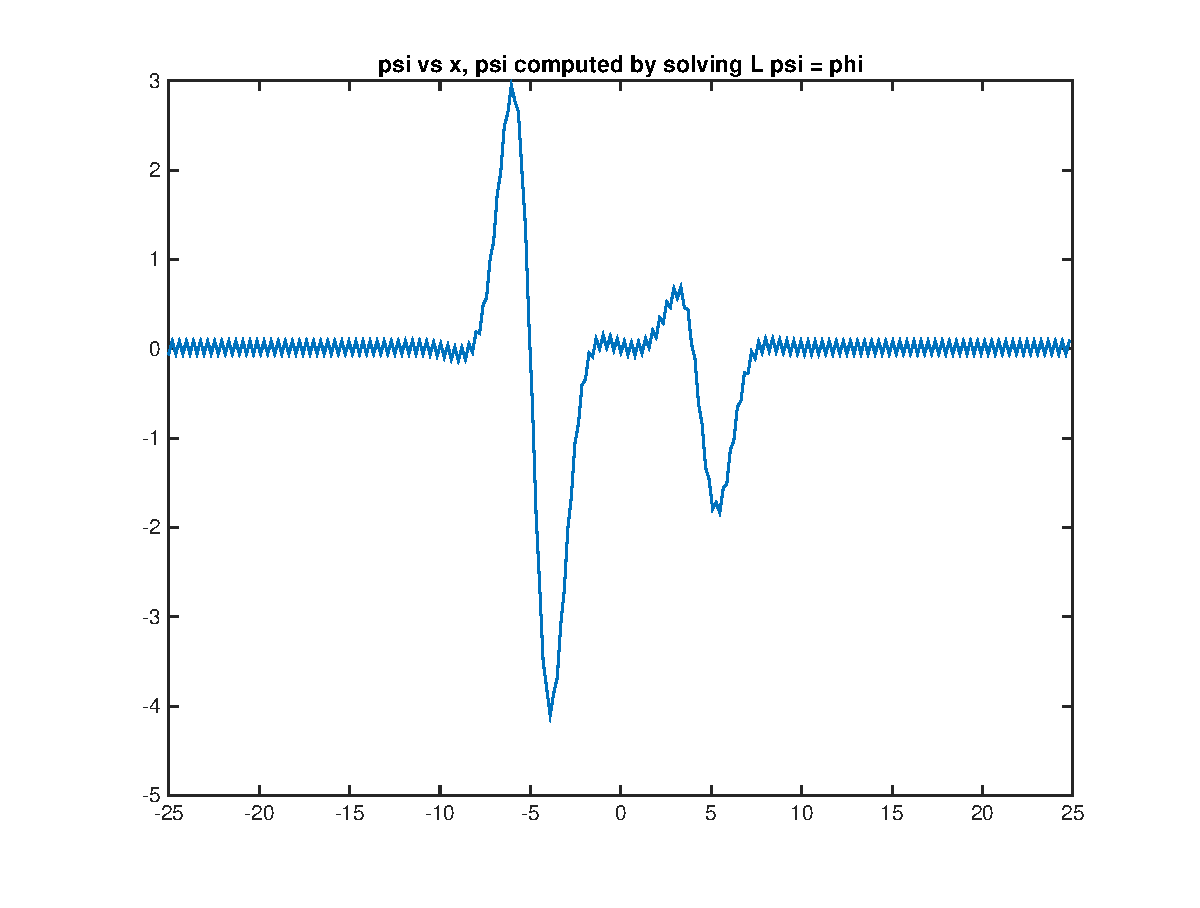
\includegraphics[width=8.5cm]{solvedpsi.eps}
\end{figure}

In this case, however, we know exactly what $\psi$ is. If we plug the stationary solution $u^*(x)$ into the original 5th order KdV equation and differentiate with respect to the speed $c$, after a little algebra we get

\begin{equation}
L(-u^*_c) = u^*_x
\end{equation}

so the generalized kernel function is $\psi = -u^*_c$. We can compute this with finite differences. Using a 1st order centered difference method with step size 0.01, we have the following plot for $u_c$:

\begin{figure}[H]
	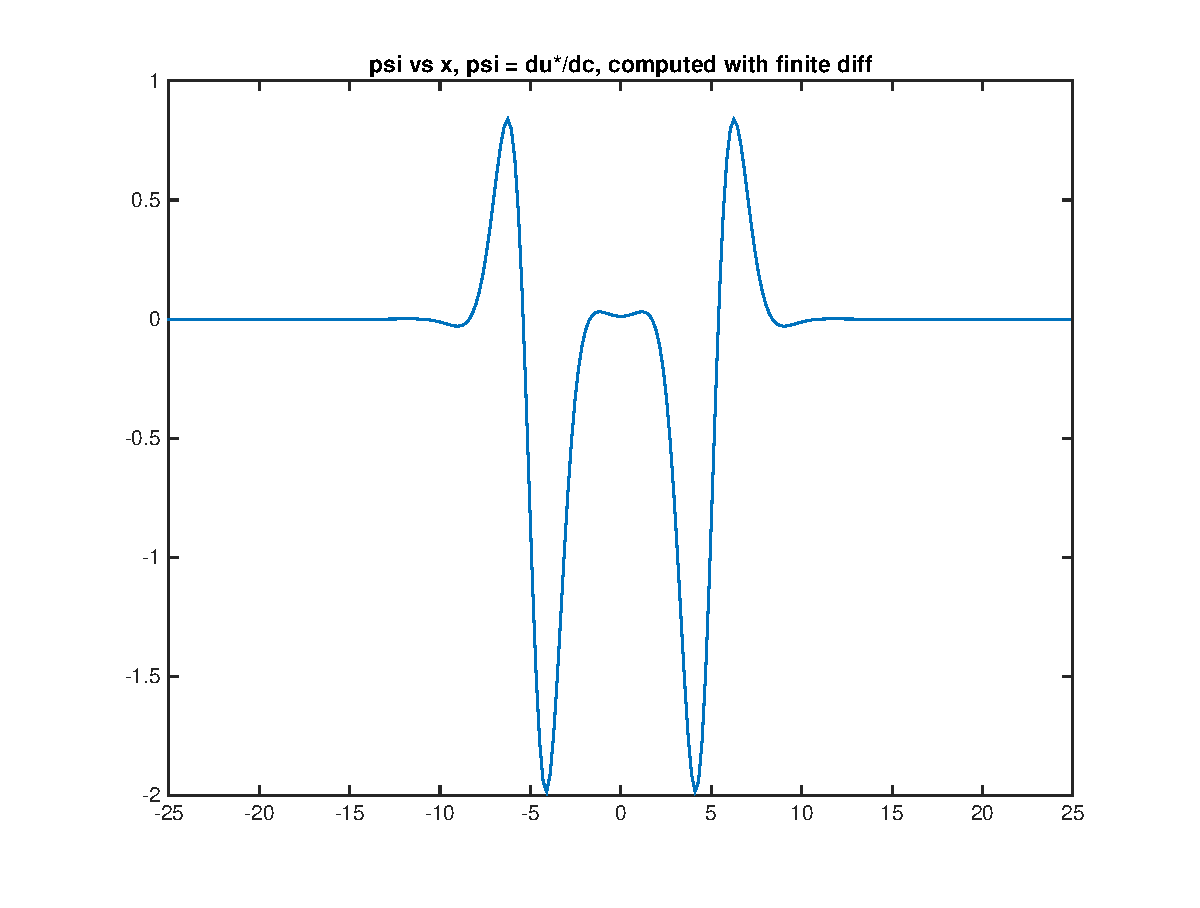
\includegraphics[width=8.5cm]{fdpsi.eps}
\end{figure}

This looks much less noisy, which is good. It also looks essentially the same for different step sizes. If we take $\phi = u^*_x$ (instead of the eigenfunction found with \texttt{eig}), then:

\begin{enumerate}
	\item For $\psi$ found by solving $L \psi = \phi$, $\max{|L \psi - \phi|} = 5.0213e-10$ 
	\item For $\psi$ found by computing $\psi = -u_c$ by finite differences $\max{|L \psi - \phi|} = 8.4471e-07$
\end{enumerate}

So this should be okay. We could probably use \texttt{fsolve} to find a ``better'' $\psi$ if we like, but this should do for now. 

\subsection{Hamilton-Krein Index}

Now we look at the ``matrix'' $D$ which is defined on the top of p. 1371 in Kapitula (2012). It is actually 1x1, i.e. a scalar, since the kernel of $H$ is one-dimensional, so will will call it $d$ to avoid confusion with the Fourier differentiation operator. This scalar is defined as:

\begin{align}
d &= <\psi, H \psi>\\
&= <-u^*_c, H (-u^*_c) >\\
&= <u^*_c, H u^*_c>
\end{align}

We can simplify this a little since we know that $L(u^*_c) = -u^*_x$, i.e. $\partial_x H(u^*_c) = -u^*_x$. Integrating this once (using the fact that our pulses and all their derivatives decay to 0 at $\pm \infty$), we get $H(u^*_c) = -u^*$. Substituting this above, we obtain:
\[
d = -<u^*_c, u^*>
\]

We want this to be negative to be consistent with what we know. (Will explain why below). Maybe there's a way to show this analytically, but I haven't thought of or found it. We can compute this numerically, though. Using \texttt{eig}, we can find $\phi$ (alternatively, we can just take the derivative of the pulse). We found $\psi$ above by finite differences. The we can compute 

\[
d = <\psi, u^*>
\]

where $u^*$ is our pulse solution (that we found numerically). If we do this for Double Pulse 2(3) (which we think is stable), speed $c = 10$, Fourier spectral methods, $N = 256$, domain size $L = 25$, we get $d = -292.5693$ for $\psi$. This is negative, so it's what we want.\\

Why do we want this to be negative? From Kapitula p. 1371-1372, we have
\begin{equation}
K_{ham} = n(H) - n(d) = k_r + 2 k_c + 2 k_i^i
\end{equation}
where $n(H)$ is the number of negative eigenvalues of $H$ and $n(d)$ is the number of negative ``eigenvalues'' of $d$, i.e. is 1 if $d$ is negative and 0 otherwise. The three things on the RHS are: the number of positive real eigenvalues of $L$ ($k_r$); the number of complex eigenvalues of $L$ with positive real and imaginary parts, i.e. eigenvalues in the first quadrant of the complex plane ($k_c$); and the number of eigenvalues of $L$ on the positive imaginary axis which have negative Krein signature $k_i^-$. \\

From our numerics (and other references, such as Chugunova and Pelinovsky (2007)), we know $n(H)$.

\begin{enumerate}
	\item $n(H) = 3$ for ``stable'' double pulses (eigenvalues of $L$ near or on imaginary axis)
	\item $n(H) = 2$ for ``unstable'' double pulses (eigenvalues of $L$ on real axis)
\end{enumerate}

If $K_{ham}$ is odd, then we must have $k_r > 0$. We know this is the case for ``unstable'' double pulses but not for ``stable'' double pulses. If $n(d) = 1$, then we get the values of $K_{ham}$ which we see numerically, i.e.

\begin{enumerate}
	\item $K_{ham} = 2$ for ``stable'' double pulses
	\item $K_{ham} = 1$ for ``unstable'' double pulses
\end{enumerate}

We understand the ``unstable'' case. For the ``stable'' case, we could get $K_{ham} = 2$ either from an eigenvalue $\alpha + i \beta$, $\alpha, \beta > 0$ (we do not think this is the case) or an eigenvalues $\beta i$, $\beta > 0$ which has negative Krein signature. The numerics suggest the second possibility.

\subsection{Krein Matrix}

Kapitula next defines the Krein Matrix. We follow the derivation in Kapitula (2010) since it has more intermediate steps, but it is the same in both papers. In the papers, the operator $J$ is boundedly invertible, whereas in our case, $J = \partial_x$ is not. We will ``pretend'' that it is invertible for now and go through the derivation formally to see if we get anything useful.\\

We consider the eigenvalue problem
\[
J H u = \lambda u
\]

where $H$ is defined above, and $J = \partial_x$. (Kapitula uses $L$ instead of $H$, but this notation is consistent with our prior work.) Let's pretend that $J$ is invertible, and define $v = J^{-1}u$. For example, $Ju = u_x$ and $J^{-1}u_x = u$. We are basically ignoring that $J$ has a one-dimensional kernel consisting of constant functions. Define the operators

\begin{align}
H_+ &= H \\
H_- &= -JHJ
\end{align}

Then both of $H_+$ and $H_-$ are self-adjoint, and the eigenvalue problem becomes

\begin{align}
H_+ u &= \lambda v \\
H_- v &= -JHu = -\lambda u
\end{align}

Now we want to write an equivalent eigenvalue problem for which the two operators $H_+$ and $H_-$ have a trivial kernel. Since $\ker H_+ = \ker H = \spn \{u^*_x\}$, the kernel of $H_+$ is one-dimensional. We would also like the kernel of $H_-$ to be one-dimensional, as in Kapitula, where we have $\ker H_- = J^{-1} \ker H_+$. It is easy to see that $u^* \in \ker H_-$. However, we the kernel of $H_-$ also contains the one-dimensional subspace of constant functions, so in fact $\ker H_- = \spn \{u^*, 1\}$. In the discrete setting, this will be a little different, as will be discussed below.\\

Note also that:
\[
<u^*, u^*_x> = \int_{-\infty}^{\infty}u^* u^*_x dx = \int_{-\infty}^{\infty} \left(\frac{1}{2} (u^*)^2\right)_x dx = 0 
\]

since the solution $u^*$ decays to 0 at $\pm \infty$.\\

Let $Z = \{u^*, u^*_x\}^\perp$ and let $\Pi: X \rightarrow Z$ be the orthogonal projection onto $Z$. Then for nonzero eigenvalues, our eigenvalue problem is equivalent to 

\begin{align}
\Pi H_+ \Pi u &= \lambda v \\
\Pi H_- \Pi &= -JHu = -\lambda u
\end{align}

The operators $\Pi H_\pm \Pi$ are self-adjoint, and since $d \neq 0$, each one is nonsingular on $Z$. Thus we can define the invertible, self-adjoint operators on $Z$

\begin{align}
R &= \Pi H_+ \Pi  \\
S^{-1} &= \Pi H_- \Pi
\end{align}

Substituting these into the eigenvalue problem, we get
\begin{align}
R u &= \lambda v \\
S^{-1} v &= -\lambda u
\end{align}

Now we rewrite this, as in Kapitula, by multiplying the second equation by $S$ to get $v = -\lambda S u$ and substituting this into the first to get the equation in $\lambda^2$ (quadratic pencil)
\[
(R + \lambda^2 S)u = 0
\]
So solving the original eigenvalue problem is equivalent to solving
\[
(R - zS)u = 0
\]

where $z = \lambda^2$, $-\pi/2 < \arg \lambda \leq pi/2$. The Krein matrix is a matrix-valued function which is singular precisely for the nonzero values of $z$ for which $(R - zS)u = 0$.\\

To construct this, we follow Kapitula (2010) as well. Let $\{\phi_j\}$ be an orthonormal eigenfunction basis for $S$ with corresponding eigenvalues $\lambda_j$. Then since $S$ is nonsingular, there are no zero eigenvalues. It was shown that $S$ has exactly $K_{ham}$ negative eigenvalues, and in our case (stable double pulse), $K_{ham} = 2$. Thus we can write the eigenvalues as $\lambda_1 \leq \lambda_2 < 0 < \lambda_3 \leq \lambda_4 \leq \cdots$. Let $N(S)$ be the 2-dimensional negative subspace of $S$. Let $P$ be the orthogonal projection on $N(S)^\perp$ and $Q = I - P$ be the orthogonal projection on $N(S)$, i.e.

\begin{align}
Pu &= u - <u,\phi_1>\phi_1 - <u, \phi_2>\phi_2 = u - \sum_{j=1}^2 <u, \phi_j>\phi_j\\
Qu &= <u,\phi_1>\phi_1 + <u, \phi_2>\phi_2 = \sum_{j=1}^2 <u, \phi_j>\phi_j
\end{align}

Define the operators
\begin{align}
R_2 &= PRP \\
S_2 &= PSP
\end{align}

Letting $p = Pu$, write $u = p + \sum_{j=1}^2 \alpha_j \phi_j \in N(S)^\perp \oplus N(S)$ for some constants $\alpha_j$. Then substitute this into the eigenvalue problem $(R - zS)u = 0$ and apply the projection $P$ to the left to get

\begin{align}
0 = P(R - zS)u &= P(R - zS)(p + \sum_{j=1}^2 \alpha_j \phi_j) \\
&= P(R - zS)Pp + P(R - zS)\sum_{j=1}^2 \alpha_j \phi_j \\
&= (R_2 - z S_2)p + \sum_{j=1}^2 \alpha_j P R \phi_j
\end{align}

where we use the fact that $P^2 = P$ since $P$ is a projection and the fact that the $\phi_j$ are eigenfunctions for $S$, so $P S\phi_j = 0$ for $j = 1, 2$.\\

We can also apply the projection $Q$ to our eigenvalue problem $(R - zS)u = 0$.

\begin{align}
0 = Q(R - zS)u &= Q(R - zS)(p + \sum_{j=1}^2 \alpha_j \phi_j) \\
&= QRp + \sum_{j=1}^2 \alpha_j Q(R - zS) \phi_j \\
&= QRp + \sum_{j=1}^2 \alpha_j Q R \phi_j - \sum_{j=1}^2 \alpha_j z \lambda_j Q \phi_j \\
&= QRp + \sum_{j=1}^2 \alpha_j Q R \phi_j - \sum_{j=1}^2 \alpha_j z \lambda_j \phi_j \\
\end{align}

where we used the fact that the projection $Q$ acts as the identity on $N(S)$ and the fact that $Sp \in N(S)^\perp$ (invariance of eigenspaces), so that $QSp = 0$. Now we take the inner product of this with $\phi_l$ for $l = 1, 2$, i.e. for $\phi_1, \phi_2$.

\begin{align}
0 &= <QRp, \phi_l> + \sum_{j=1}^2 \alpha_j <Q R \phi_j, \phi_l> - \sum_{j=1}^2 \alpha_j z \lambda_j <\phi_j, \phi_l>
\end{align}

Using the fact that the projection $Q$ is self-adjoint, $Q \phi_j = \phi_j$ for $j = 1, 2$ (since $Q$ acts as the identity on $N(S)$), and the fact that the basis $\{phi_j\}$ is orthonormal, we get for $l = 1, 2$

\begin{align}
<Rp, Q\phi_l> + \sum_{j=1}^2 \alpha_j <R \phi_j, Q\phi_l> &= \sum_{j=1}^2 \alpha_j z \lambda_j <\phi_j, \phi_l> \\
<Rp, \phi_l> + \sum_{j=1}^2 \alpha_j <R \phi_j, \phi_l> &= \alpha_l z \lambda_l
\end{align}

So we have the following system of equations to deal with

\begin{align}\label{system}
(R_2 - z S_2)p + \sum_{j=1}^2 \alpha_j P R \phi_j &= 0 \\
<Rp, \phi_l> + \sum_{j=1}^2 \alpha_j <R \phi_j, \phi_l> &= \alpha_l z \lambda_l && l = 1, 2
\end{align}

The idea is that we will solve for $p$ in the first equation and substitute that into the second equation. Since $S_2$ is positive definite (by construction), $S_2 = S_2^{1/2} S_2^{1/2}$ is well-defined. By using this and doing a little algebra, we get

\begin{align}
R_2 - z S_2 &= S_2^{1/2} S_2^{-1/2} R_2 S_2^{-1/2} S_2^{1/2} - S_2^{1/2} z S_2^{1/2} \\
&= S_2^{1/2} ( S_2^{-1/2} R_2 S_2^{-1/2} - z I ) S_2^{1/2} \\
&= S_2^{1/2} ( \tilde{R} - z I ) S_2^{1/2} 
\end{align}

where $\tilde{R} = S_2^{-1/2} R_2 S_2^{-1/2}$, and $\tilde{R}: N(S)^\perp \rightarrow N(S)^\perp$ since $R_2, S_2: X \rightarrow N(S)^\perp$ and $S_2$ is invariant on $S_2^\perp$. $\tilde{R}$ is self-adjoint since it is the product of self-adjoint operators. $\tilde{R}$ and $R_2$ also have the same sized negative eigenspace, I think because multiplying by a positive definite operator on both sides does not affect this. $\tilde{R}$ also apparently has compact resolvent, so as long as $z$ is not in the spectrum of $\tilde{R}$, the operator $( \tilde{R} - z I )^{-1}$ is well defined and is bounded. In any case, we have an expression for $R_2 - zS_2$, so we can substitute this into the first equation of \eqref{system} to get

\[
S_2^{1/2} ( \tilde{R} - z I ) S_2^{1/2} p + \sum_{j=1}^2 \alpha_j P R \phi_j = 0 
\]

The steps to invert this (and what we do in the case that $z$ is in the spectrum of $\tilde{R}$ are given in Kaptiula (2010). After doing, the Krein matrix is defined on the bottom of p.1253 in Kapitula (2010). The nice thing is that it is 2x2 in our case, so it should not be hard to deal with, assuming we can compute it numerically to any degree of accuracy. We define the following three matrices, for $j, l = 1, 2$:

\begin{align}
\hat{R}_{jl} &= <\phi_j, R \phi_l> \\
D &= \textrm{diag}(\lambda_1, \lambda_2) \\
C(z)_{jl} &= <S_2^{-1/2}(\tilde{R} - zI)^{-1} S_2^{-1/2} P R \phi_j, P R \phi_l>
\end{align}

The first two are straightforward, which is nice. The Krein matrix is defined by 
\begin{equation}\label{kreinmatrix}
K(z) = \hat{R} - zD - C(z)
\end{equation}

We can simplify things a bunch by getting rid of the $\tilde{R}$, since

\begin{align}
S_2^{-1/2}(\tilde{R} - zI)^{-1} S_2^{-1/2} &= (S_2^{1/2})^{-1}(\tilde{R} - zI)^{-1} (S_2^{1/2})^{-1} \\
&= ( S_2^{1/2} ( \tilde{R} - zI ) S_2^{1/2} )^{-1} \\
&= ( S_2^{1/2} ( S_2^{-1/2} R_2 S_2^{-1/2} - zI ) S_2^{1/2} )^{-1} \\
&= ( R_2 - z S_2 )^{-1}
\end{align}

Thus the definition of the Krein matrix becomes

\begin{align}\label{kreinmatrixsimple}
\hat{R}_{jl} &= <\phi_j, R \phi_l> \\
D &= \textrm{diag}(\lambda_1, \lambda_2) \\
C(z)_{jl} &= < ( R_2 - zS_2 )^{-1} P R \phi_j, P R \phi_l> \\
K(z) &= \hat{R} - zD - C(z)
\end{align}

This is much easier to compute.\\

What does all of this mean? First, note the correspondence between the eigenvalue $z$ of the problem $(R - zS)u = 0$ and our original eigenvalue problem $JLu = \lambda u$. We only care about the potentially unstable eigenvalues $\lambda$ here, which is why, say, $\lambda \in \R^-$ is not involved.
\begin{enumerate}
	\item $\lambda \in \R^+ \iff z \in \R^-$
	\item $\textrm{Im} \lambda \neq 0$ and $\textrm{Re} \lambda > 0 \iff \textrm{Im} z \neq 0$
	\item $\lambda \in i\R^+ \iff z \in \R^+$  
\end{enumerate}

Note that $\lambda \in i\R^-$ is not included here, but that's ok by symmetry since if $\lambda$ is an eigenvalue, so is its complex conjugate. Given all this, I believe the following statements are true about the Krein matrix. 

\begin{enumerate}
	\item If $\textrm{Im} z \neq 0$, then $\det K(z) = 0 \iff z$ is an eigenvalue (complex eigenvalue with positive real part, nonzero imaginary part).
	\item If $z \in \R^+$ with negative Krein signature, then $\det K(z) = 0$ (eigenvalue on the positive imaginary axis).
	\item We don't have to care about the case when $z \in \R^-$ since that corresponds to a positive real eigenvalue $\lambda$, and we know that is not the case for our unstable double pulse.
\end{enumerate}

\section{Krein Matrix, computations (22 July 2017)}

Now that we know how the Krein matrix could be defined in our context, we will (attempt to) compute it numerically using Matlab. First we note the following difference between the (nonrigorous) theoretical work above. The differentiation operator $\partial_x$ has the as its kernel the constant functions $\spn \{1 \}$. This is periodic for any period, so this does not change with periodic BCs. Interestingly, the kernel of the discrete Fourier collocation operator $D$ is two-dimensional. Here is a plot of the two kernel elements.

\begin{figure}[H]
	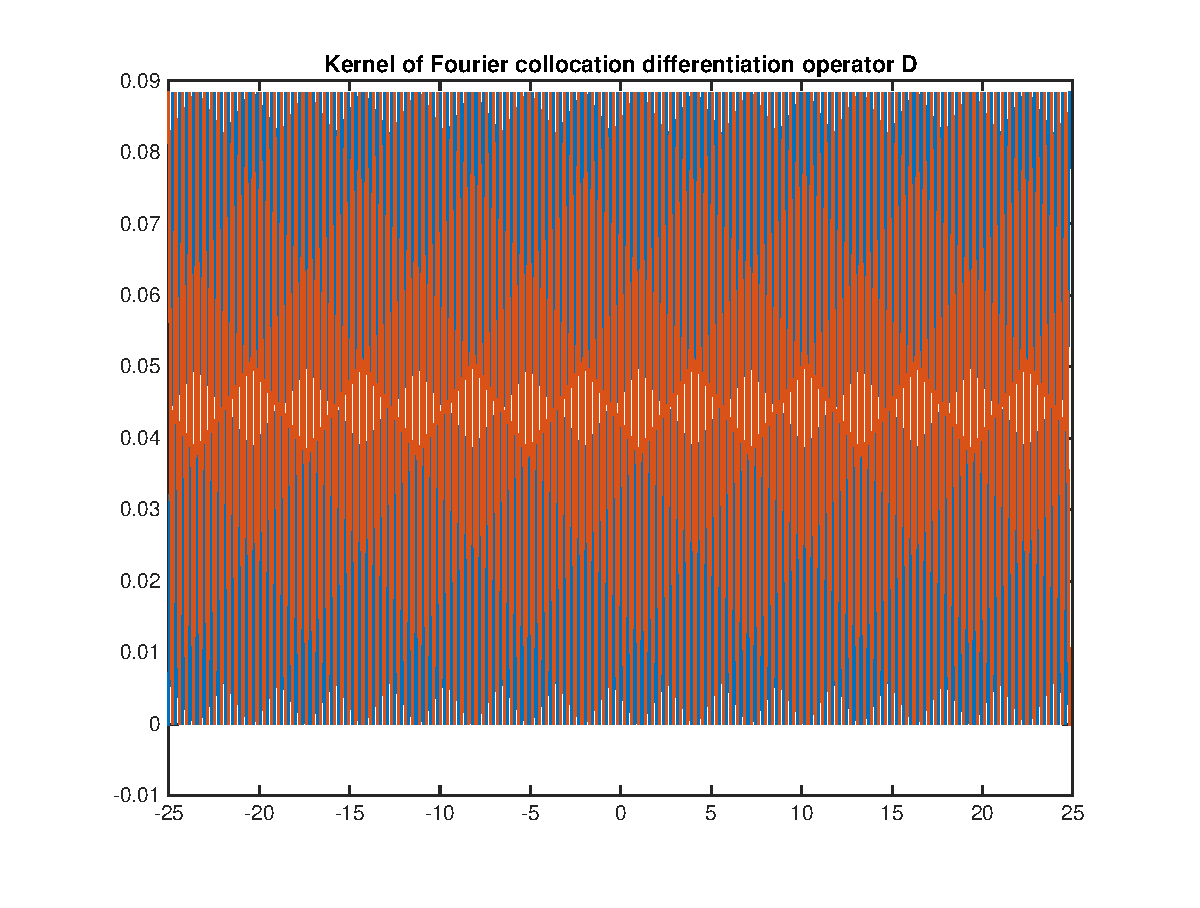
\includegraphics[width=8.5cm]{kerD}
\end{figure}

It's a little hard to see, since the oscillations are the maximum frequency we can have on a grid of this size, but the two oscillatory functions are identical except they are shifted 1 grid point horizontally relative to each other. In any case, if we take the space spanned by these functions as $\ker D$, then we get the result we want, so we will do that. Thus we have:
\begin{align}
\ker H_+ &= \spn \{ u^*_x \} \\
\ker H_- &= \spn \{u^*\} \oplus \ker D
\end{align}
Letting $\Pi$ be the orthogonal projection onto $(\ker H_+ \oplus \ker H_-)^\perp$, the rest follows as above.\\

Computing the Krein matrix is relatively straightforward. First, we will do this for the first ``stable'' double pulse, i.e. double pulse 2(3). We use Fourier spectral methods, wave speed $c = 10$, $N = 256$, $L = 50$. \\

After computing the operator $S$ as in the previous section, we look at the negative eigenspace of $S$. As predicted, $S$ has 2 negative eigenvalues. The corresponding eigenfunctions $\phi_1, \phi_2$ are shown below. One is even, and one is odd, which is what we wanted to occur (although I'm not sure why we thought this would be the case).

\begin{figure}[H]
	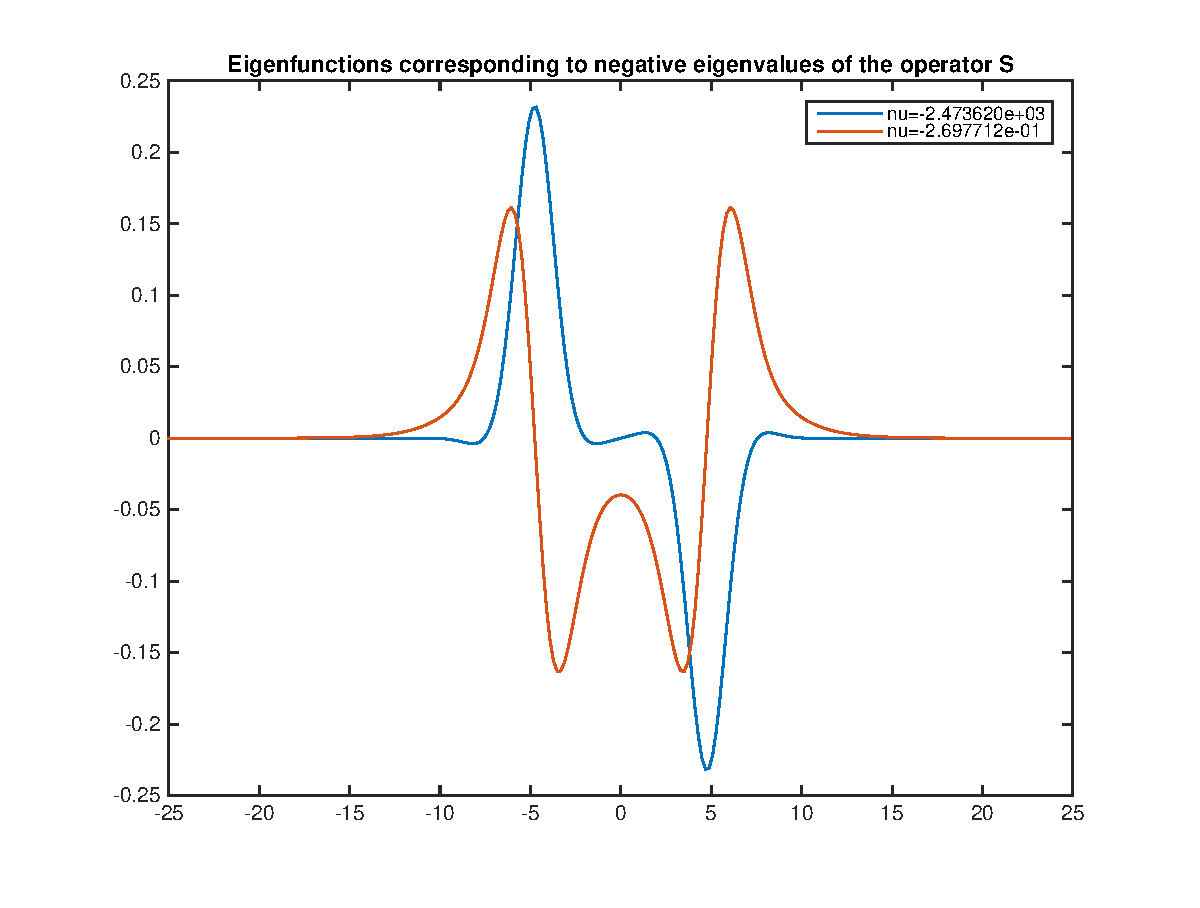
\includegraphics[width=8.5cm]{dp2vNeg}
	\caption{Eigenfunctions corresponding to negative eigenvalues of the operator S. Double pulse 2(3), wave speed $c = 10$, Fourier spectral methods, $N = 256$, $L = 50$.}
\end{figure}

The eigenfunctions corresponding to $\nu = -2.47e+03$ is odd and the eigenfunction corresponding to $\nu=-2.70e-01$ is even.\\

We can also plot the derivatives of these eigenfunctions. From this we can see that neither negative eigenfunction is the derivative of the other.

\begin{figure}[H]
	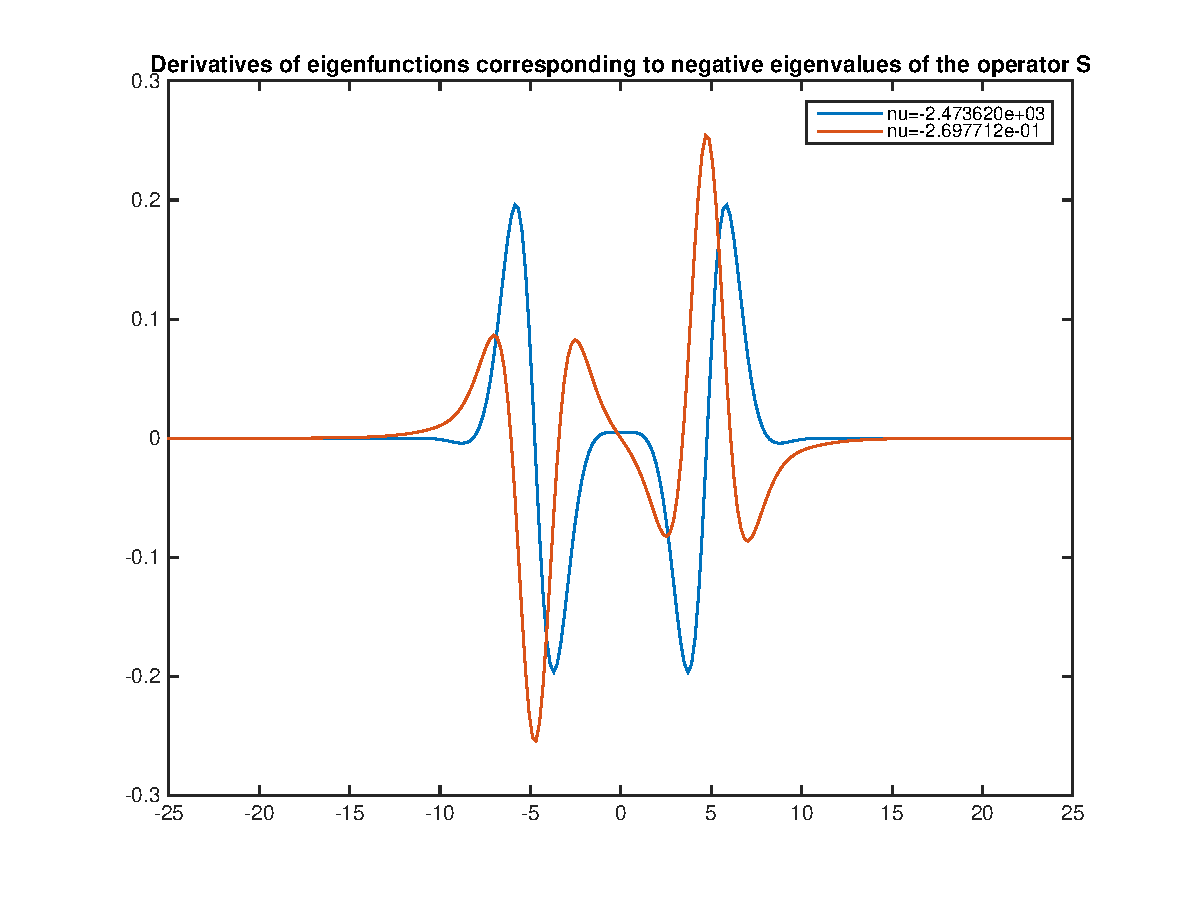
\includegraphics[width=8.5cm]{dp2dvNeg}
	\caption{Normalized derivatives of eigenfunctions corresponding to negative eigenvalues of the operator S. Double pulse 2(3), wave speed $c = 10$, Fourier spectral methods, $N = 256$, $L = 50$.}
\end{figure}

Using these eigenfunctions, we can compute the Krein matrix $K(z)$. Note that since one eigenfunction is even and one eigenfunction is odd, and since the operators $R$ and $R_2 - zS_2 )^{-1}$ are self-adjoint, the Krein matrix is diagonal, which is really nice. (The Krein matrix is known to be symmetric, so what we have here is a special case of that.) As an example, for $z = 1$, the Krein matrix (for the same conditions as above) is:

\[
K(1) = \begin{bmatrix}
2.4618e+03 & -9.9711e-10 \\ -1.0294e-09 & 0.1978
\end{bmatrix}
\]
which (to numerical accuracy) is diagonal.\\

We computed earlier that the eigenvalue on (or near) the positive imaginary axis is $\lambda = 0.0691i$; $z = \lambda^2 = 0.0048$, and for this value of $z$, $\det K(z) = -3.9567e-16$, which is essentially 0, so the Krein matrix is in fact singular at our eigenvalue, supporting our hypothesis that this eigenvalue is in fact on the imaginary axis and has negative Krein signature. \\

As in Kapitula (2013), we can look at the Krein eigenvalues, which are the eigenvalues of the Krein matrix. (Conveniently, since the Krein matrix is diagonal, these are just the diagonal entries). It is instructive to plot these as a function of $z \in \R$ (we only really care about $z \in R^+$, since that corresponds to eigenvalues $\lambda$ which are on the positive imaginary axis, but it does not hurt to do this for a symmetric interval about 0). Below is a plot of the two Krein eigenvalues for $z \in [-0.1, 0.1]$.

\begin{figure}[H]
	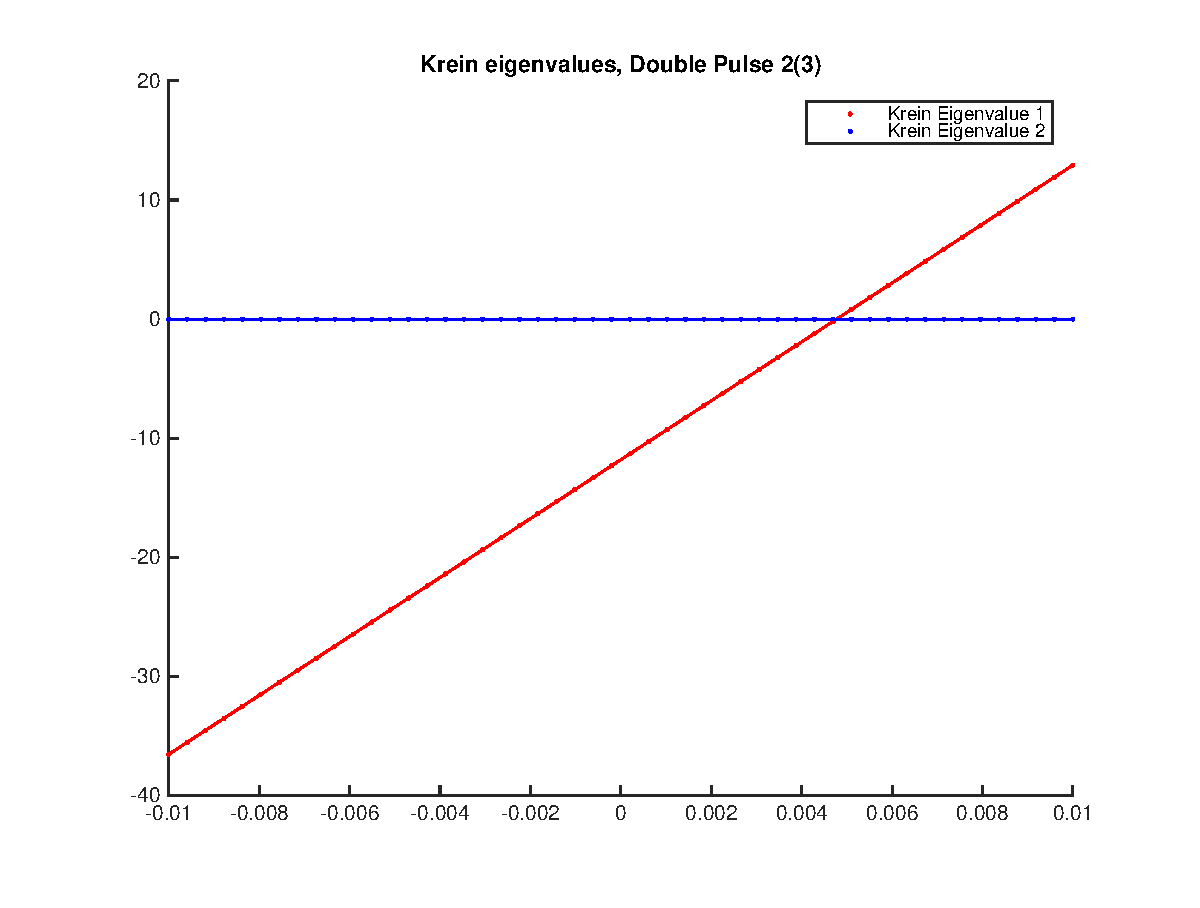
\includegraphics[width=8.5cm]{dp2kreineig1}
	\caption{Krein eigenvalues. Double pulse 2(3), $c = 10$, Fourier spectral methods, $N = 256$, $L = 50$. }
\end{figure}

Note that both Krein eigenvalues appear to be a linear function of $z$, so we also included a plot of the least squares linear interpolation of the two Krein eigenvalues on the graph. The red line has a large positive slope (2474), and crosses 0 at a single point. The blue line (Krein eigenvalue 2) actually has a small positive slope (0.2082), which is hard to see on this graph, but is apparent when graphed separately.

\begin{figure}[H]
	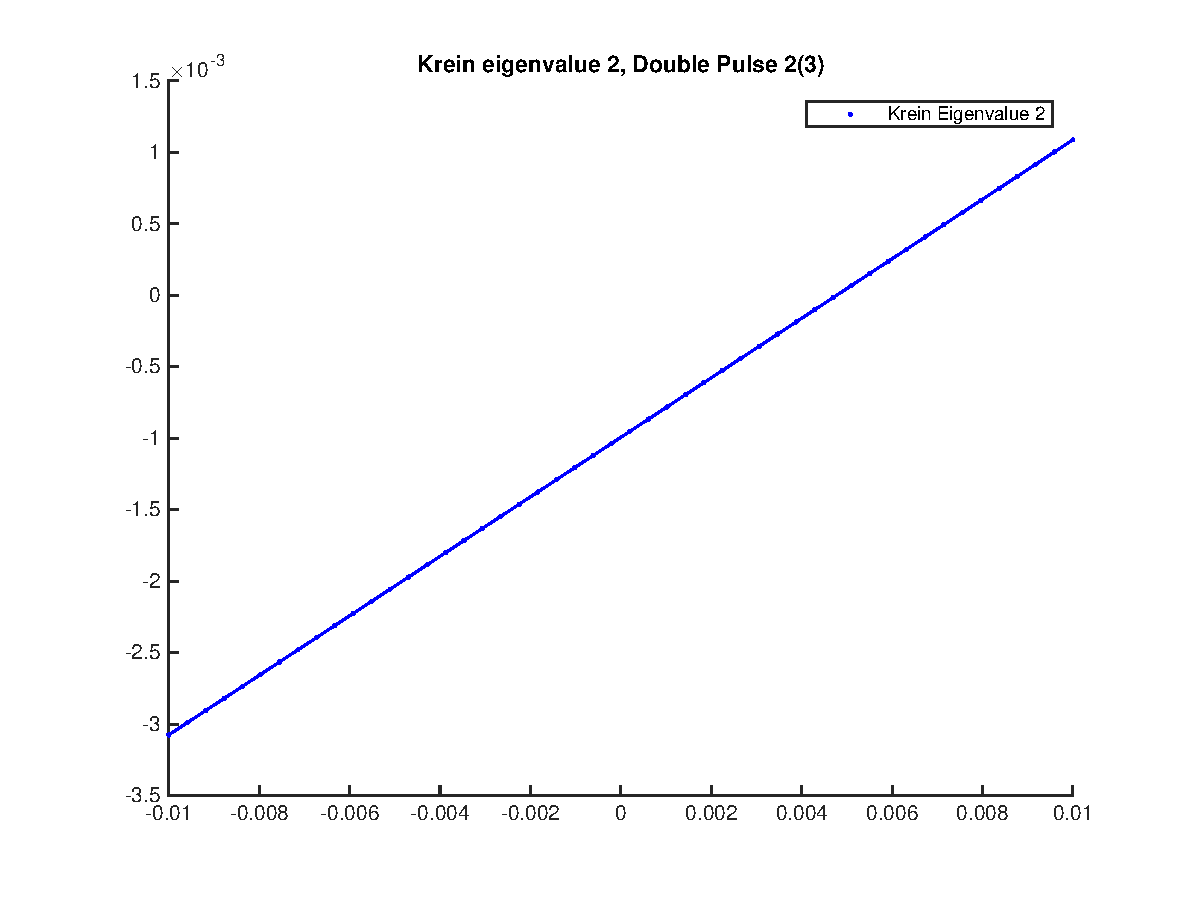
\includegraphics[width=8.5cm]{dp2kreineig2}
	\caption{Krein eigenvalue 2 only. Double pulse 2(3), $c = 10$, Fourier spectral methods, $N = 256$, $L = 50$. }
\end{figure}

We can see from the plots that the two lines cross. If we zoom in on the crossing, we can see that the two lines cross each other at the same values of $z$ for which they each cross 0!

\begin{figure}[H]
	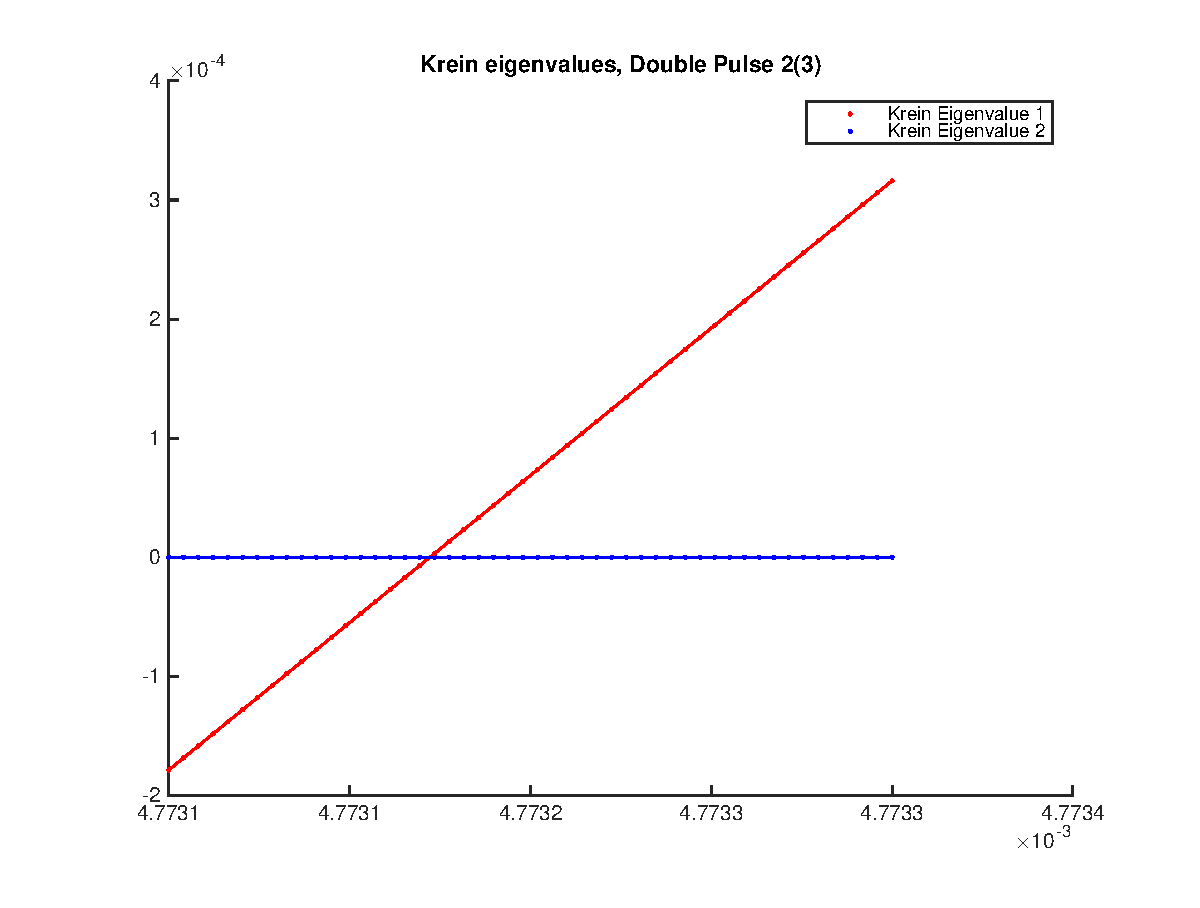
\includegraphics[width=8.5cm]{dp2kreineig1zoom}
	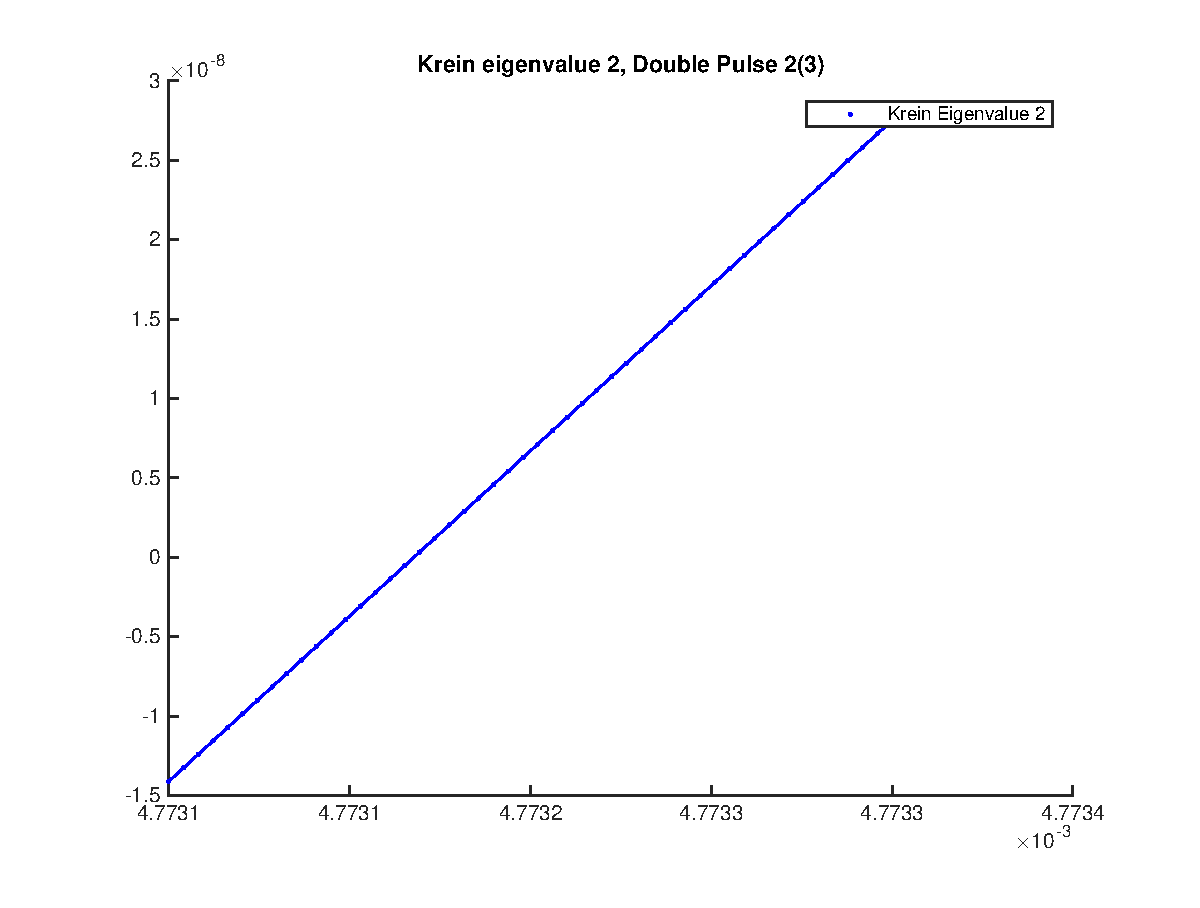
\includegraphics[width=8.5cm]{dp2kreineig2zoom}
	\caption{Krein eigenvalues, zoom on crossing. Double pulse 2(3), $c = 10$, Fourier spectral methods, $N = 256$, $L = 50$.}
\end{figure}

We can compute this crossing point numerically, which is $z = 0.0048$, and $\sqrt{z} = 0.0691$, which is the imaginary part of our interaction eigenvalue $\lambda$. At the crossing point, both eigenvalues are of order $1e-9$, which is essentially zero, and the determinant of the Krein matrix is $-1.0165e-18$, which is also essentially zero. All of this provides more evidence that we have a purely imaginary eigenvalue on the positive imaginary axis of negative Krein signature at $\lambda = 0.0691i$.\\

Of course, all of this is for nothing if we cannot reproduce these results in other situations. So let's do that. First, let's try double pulse 2(5) for the same wave speed $c = 10$, i.e. the next ``stable'' double pulse. We will not show the negative eigenfunctions of $S$, since they look similar to those above. We will go straight to the Krein eigenvalues.

\begin{figure}[H]
	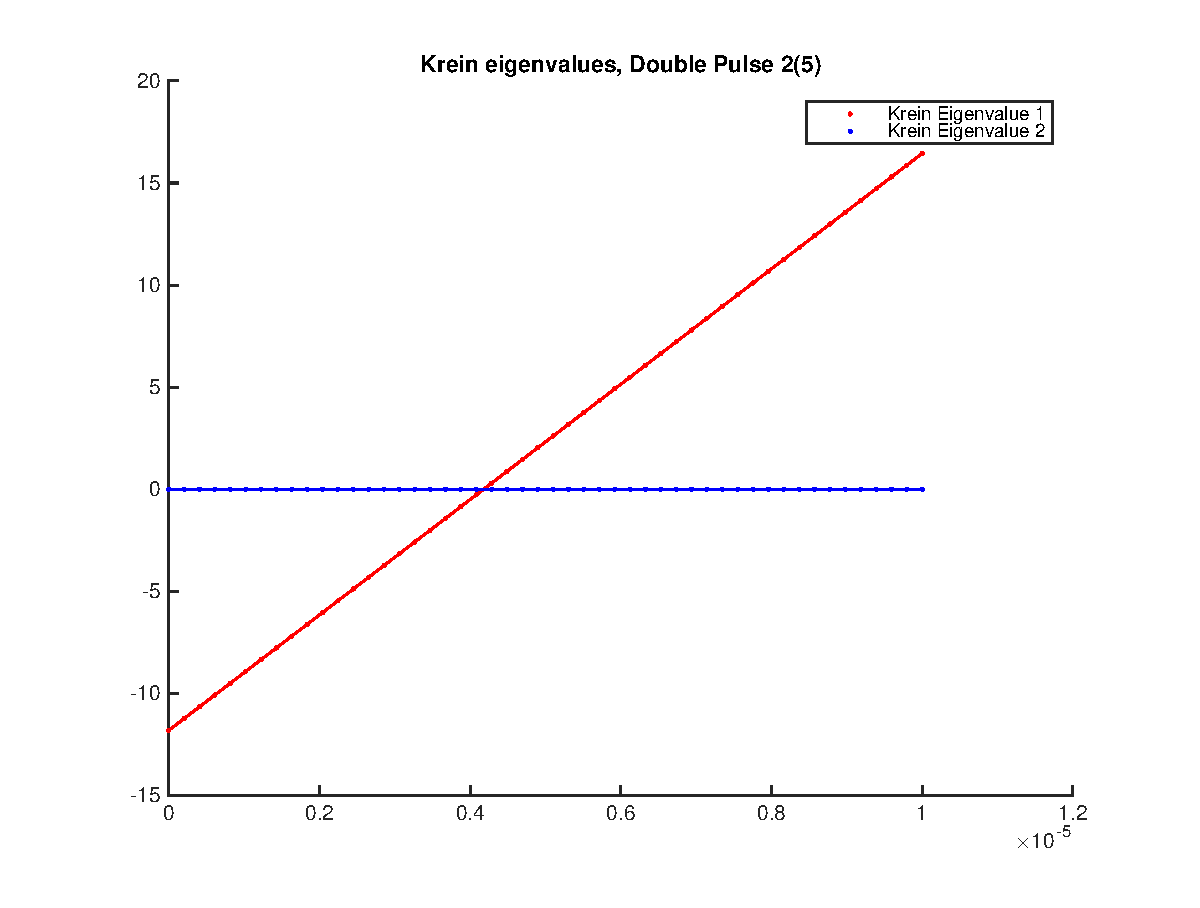
\includegraphics[width=8.5cm]{dp4kreineig1}
	\caption{Krein eigenvalues. Double pulse 2(5), $c = 10$, Fourier spectral methods, $N = 256$, $L = 50$. }
\end{figure}

We once again have two straight lines with upward slope. They cross each other and zero (roughly, the numbers are getting tiny!) at $z = 4.1790e-06$, which corresponds to $\lambda = 0.0020i$, which is the interaction eigenvalue we found before.\\

There is no reason to suspect this will not work for another speed $c$, but let's do it anyway. Here we repeat this for double pulse 2(3) and $c = 7.5$.

\begin{figure}[H]
	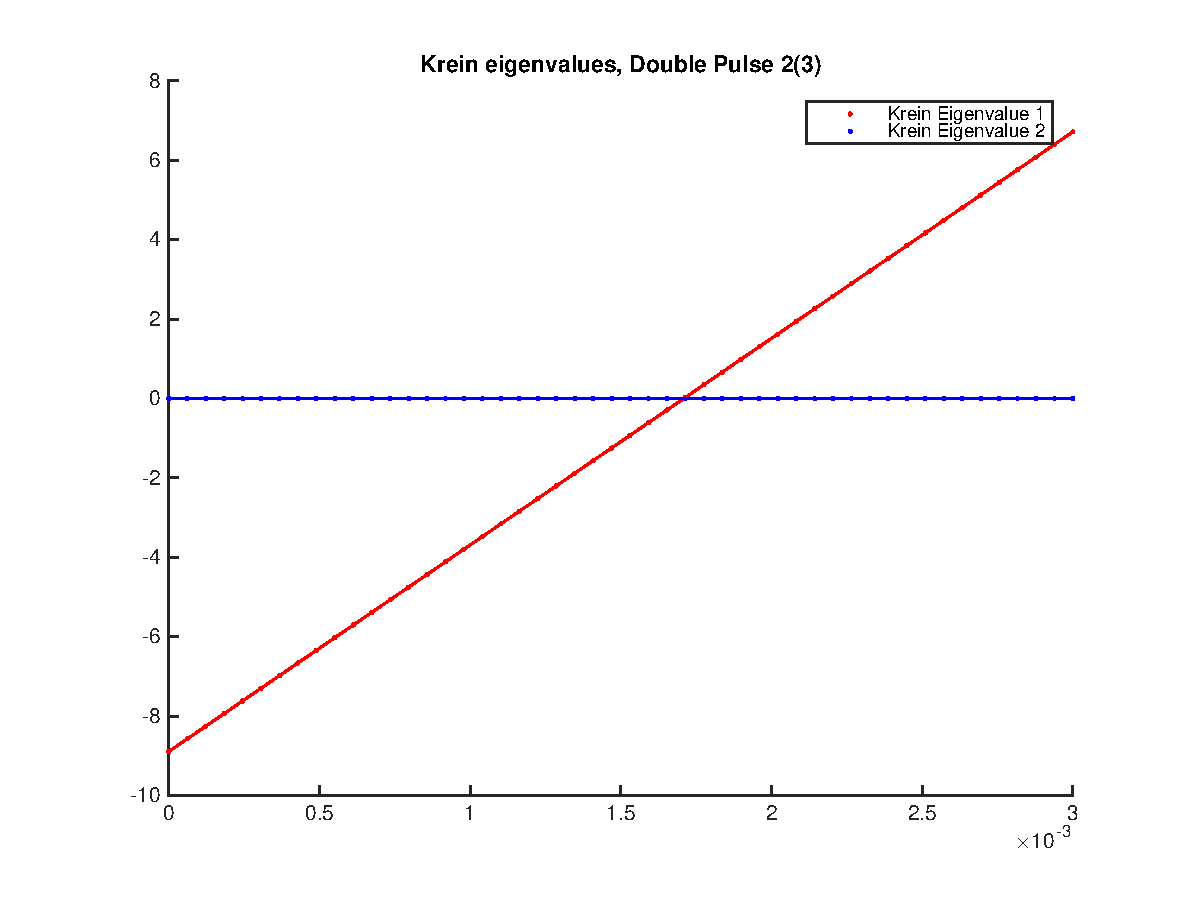
\includegraphics[width=8.5cm]{dp2_75kreineig1}
	\caption{Krein eigenvalues. Double pulse 2(3), $c = 7.5$, Fourier spectral methods, $N = 256$, $L = 50$. }
\end{figure}

Plot is similar to the two above. The crossing point for the two lines (and zero) is at $z = 0.0017$, which corresponds to the interaction eigenvalue of $\lambda = 0.0413i$, which is what we found earlier.\\

Since the Krein matrix also counts positive real eigenvalues, we should be able to use this for the unstable double pulses as well. Let's try it on double pulse 2(2), $c = 10$. For the unstable double pulses, $K_{ham} = 1$, which implies that we have to have one positive, real eigenvalue. Details are in Kapitula (2013). Thus the matrix $S$ will only have one negative eigenvalue, and so the Krein matrix will be 1x1, i.e. a scalar. Repeating all of this for the unstable double pulse 2(2), this is in fact what we see. Here is a plot of that single eigenfunction. Note that it is an even function.

\begin{figure}[H]
	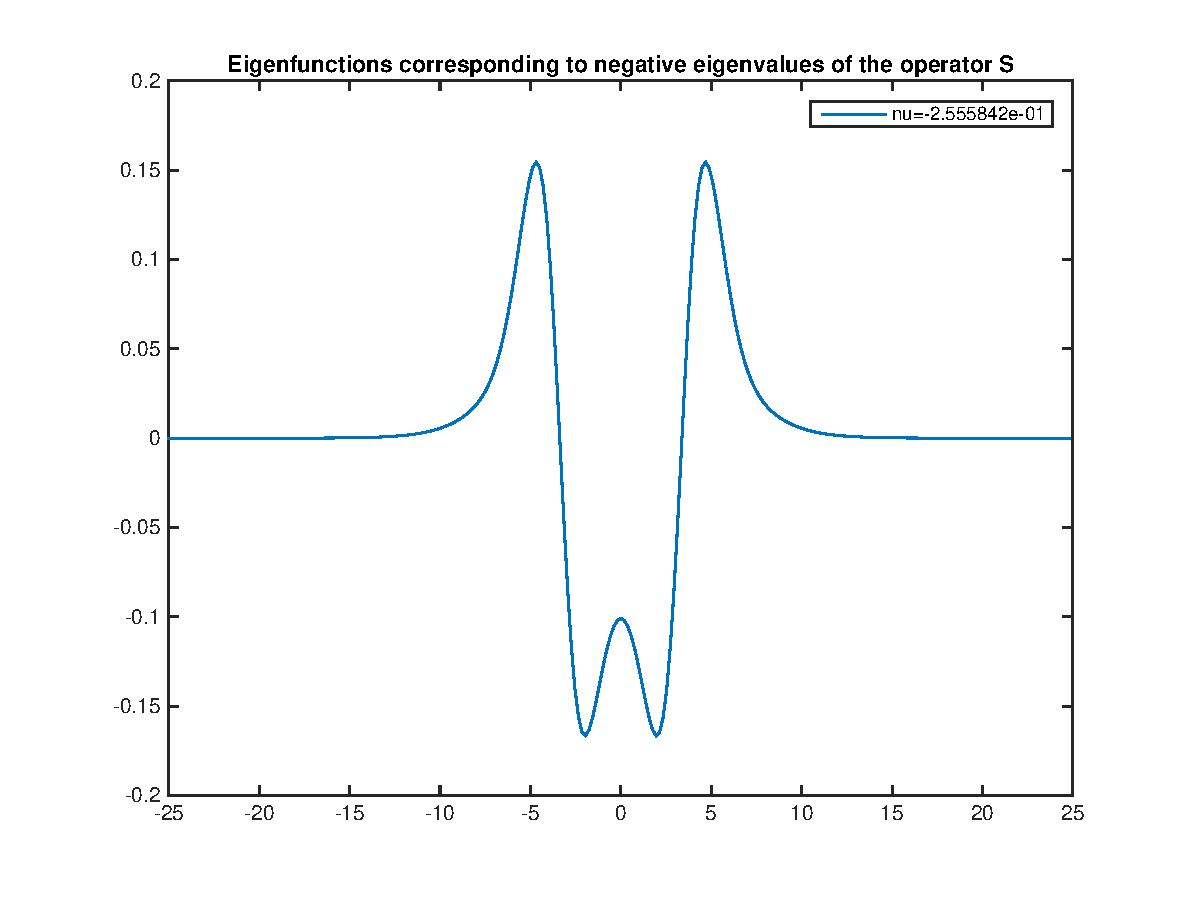
\includegraphics[width=8.5cm]{dp1vNeg}
	\caption{Eigenfunction corresponding to negative eigenvalue of the operator S. Double pulse 2(2), wave speed $c = 10$, Fourier spectral methods, $N = 256$, $L = 50$.}
\end{figure}

To find the interaction eigenvalue, all we have to do is see where the single Krein eigenvalue (which is the entire Krein matrix) crosses 0. This is shown in the plot below. Note once again the Krein eigenvalue is a linear function of $z$. 

\begin{figure}[H]
	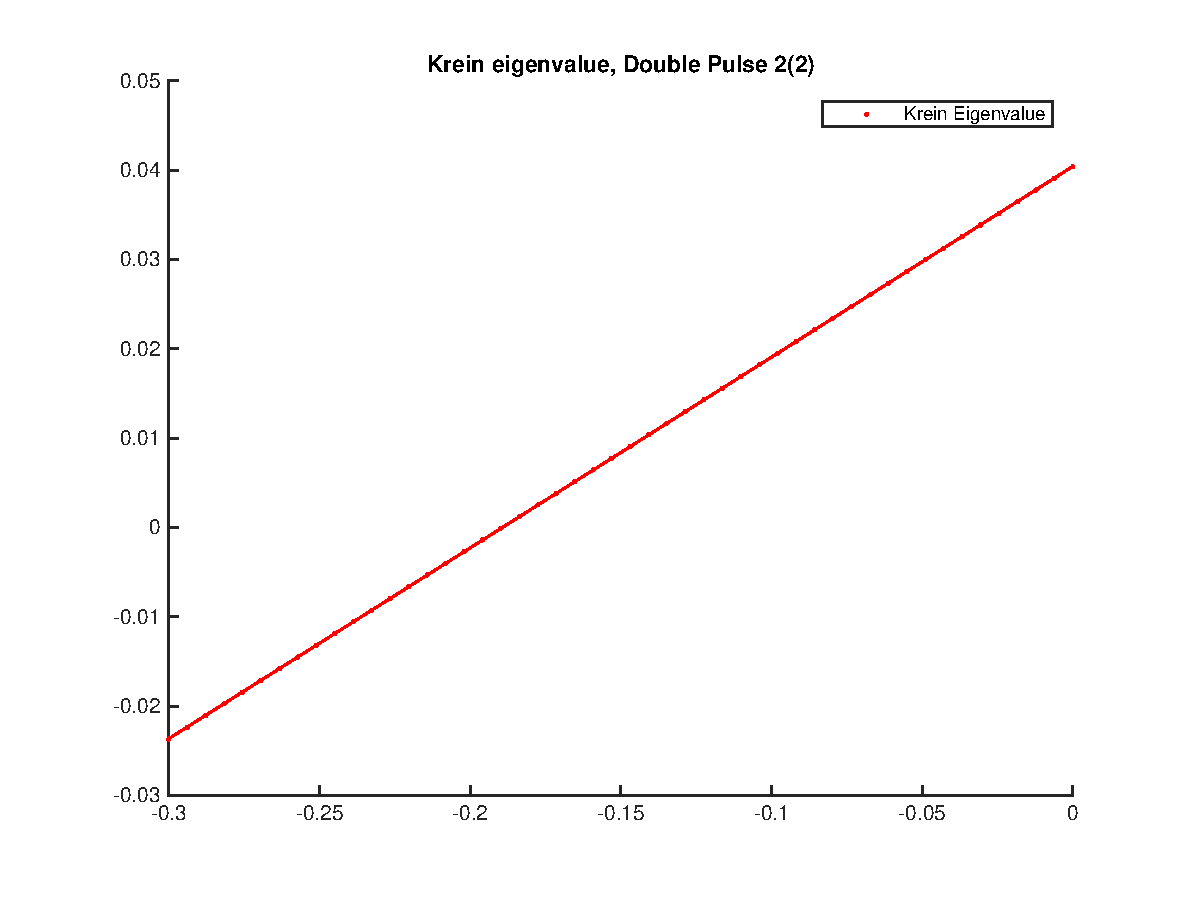
\includegraphics[width=8.5cm]{dp1kreineig1}
	\caption{Krein eigenvalue. Double pulse 2(2), $c = 10$, Fourier spectral methods, $N = 256$, $L = 50$. }
\end{figure}

The Krein eigenvalue crosses 0 at -0.1894, corresponding to an interaction eigenvalue of $\lambda = 0.4352$, which is exactly what we observed before.\\

In conclusion, even though our setup is different from that in Kapitula (2013), i.e. the operator $J$ in our case is not invertible, we can follow the same steps and construct the Krein matrix. In all cases we have tried, the Krein matrix identifies exactly the interaction eigenvalues which we found before using \texttt{eig} on the discretized operator.\\

What about the essential spectrum? We should be able to find it using the Krein matrix as well. Let's go back to double pulse 2(3), $c = 10$, $N = 256$, $L = 50$. Looking at the positive imaginary axis, the interaction eigenvalue is at $0.0691i$, and the first three eigenvalues of the essential spectrum are at $1.4164i, 2.8558i, 4.3473i$. So we need to look at higher values of $z$. This plot shows the Krein eigenvalues for $z$ ranging from 0 to 10.

\begin{figure}[H]
	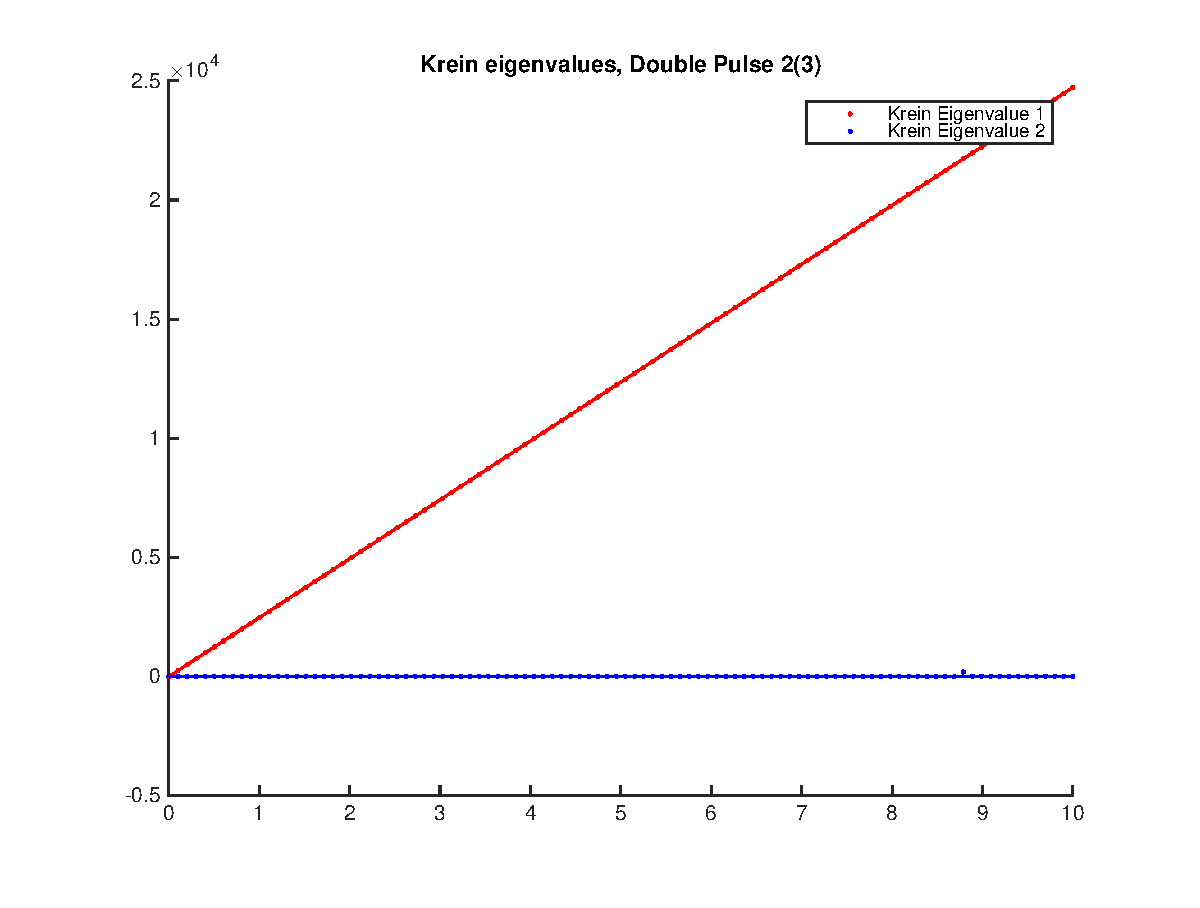
\includegraphics[width=8.5cm]{dp2kreineig3.eps}
	\caption{Krein eigenvalues, $z \in [0, 10]$. Double pulse 2(3), $c = 10$, Fourier spectral methods, $N =  256$, $L = 50$. }
\end{figure}

Krein eigenvalue 1 (red line) at first glance appears to increase linearly with $z$. This will turn out not to be the case, as there are very narrow singularities there, but let's first take a closer look at Krein eigenvalue 2 (blue line). 

\begin{figure}[H]
	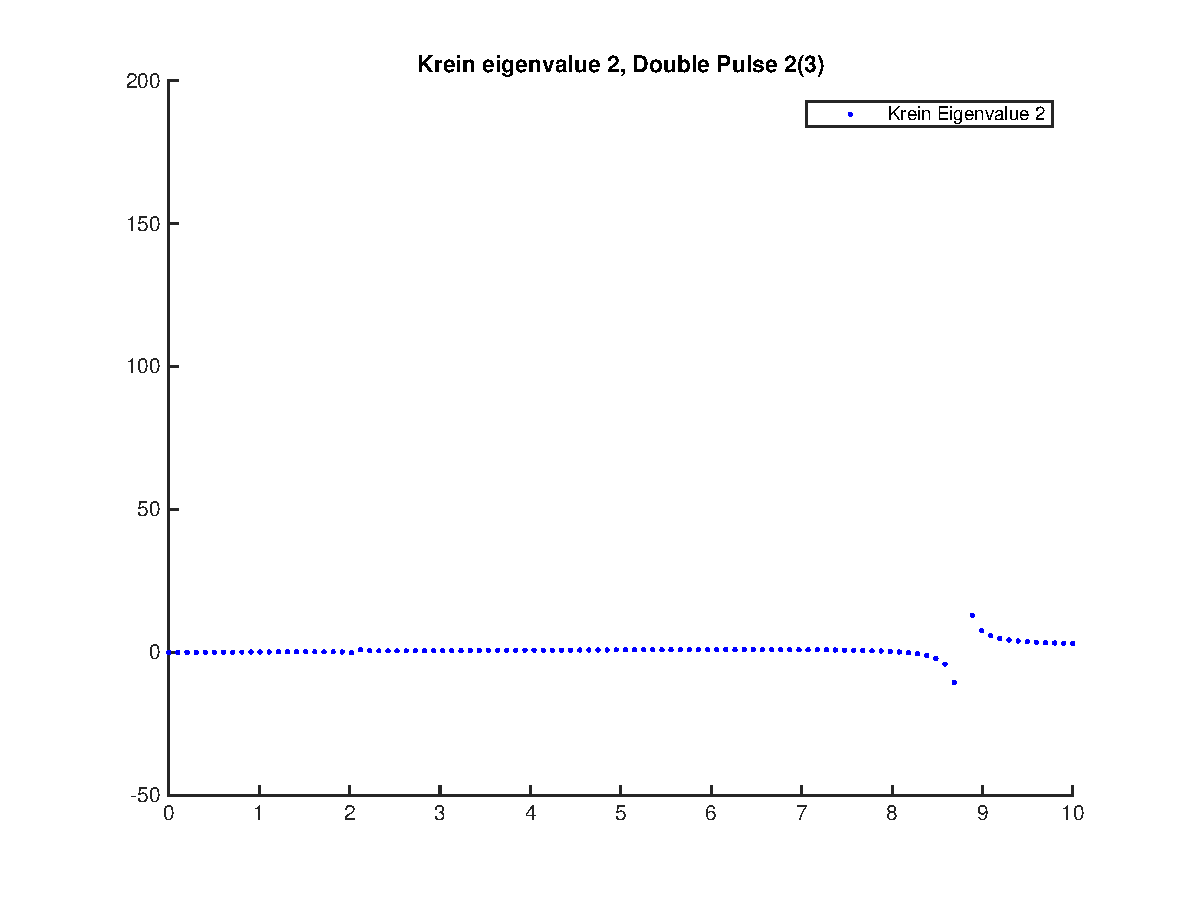
\includegraphics[width=8.5cm]{dp2kreineig4.eps}
	\caption{Krein eigenvalue 2, $z \in [0, 10]$. Double pulse 2(3), $c = 10$, Fourier spectral methods, $N =  256$, $L = 50$. }
\end{figure}

It looks like something interesting is happening around $z = 2$ and around $z = 9$. Let's first look at the interval $z \in [0, 2]$.

\begin{figure}[H]
	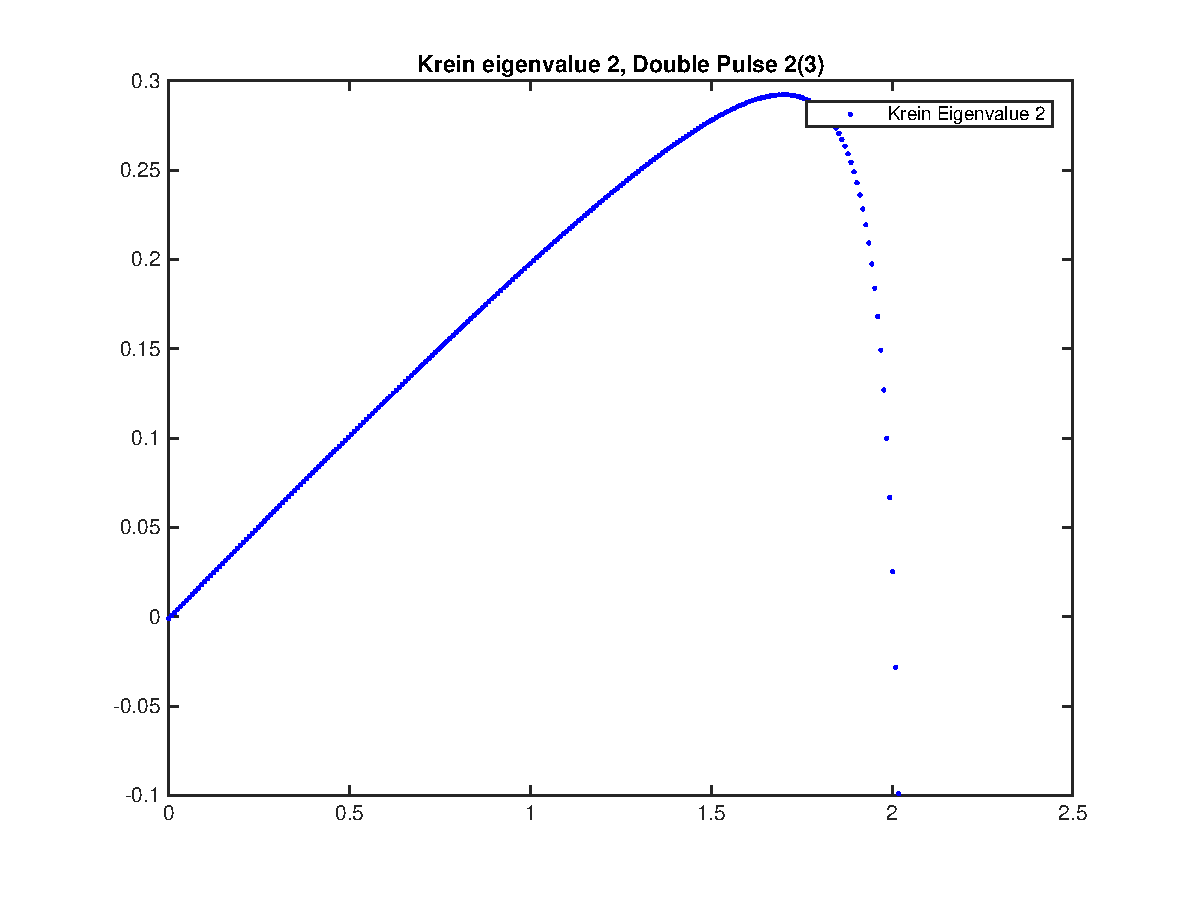
\includegraphics[width=8.5cm]{dp2kreineig0-2.eps}
	\caption{Krein eigenvalue 2, $z \in [0, 2]$. Double pulse 2(3), $c = 10$, Fourier spectral methods, $N =  256$, $L = 50$.}
\end{figure}

Note that the curve for Krein eigenvalue 2 starts with an upward slope. At $z = 0$, Krein eigenvalue 2 is negative, and the first crossing of 0 occurs at $z = 0.0048$, which is so far to the left of this graph that we really can't see it (this is clearly shown on the relevant plot above). After continuing upward until about $z = 1.75$, the curve turns downwards. There is another crossing of 0 somewhere around 2 before the curve continues to head down towards what looks like a vertical asymptote/singularity. We can zoom in around $z = 2$ to get a better look at this.

\begin{figure}[H]
	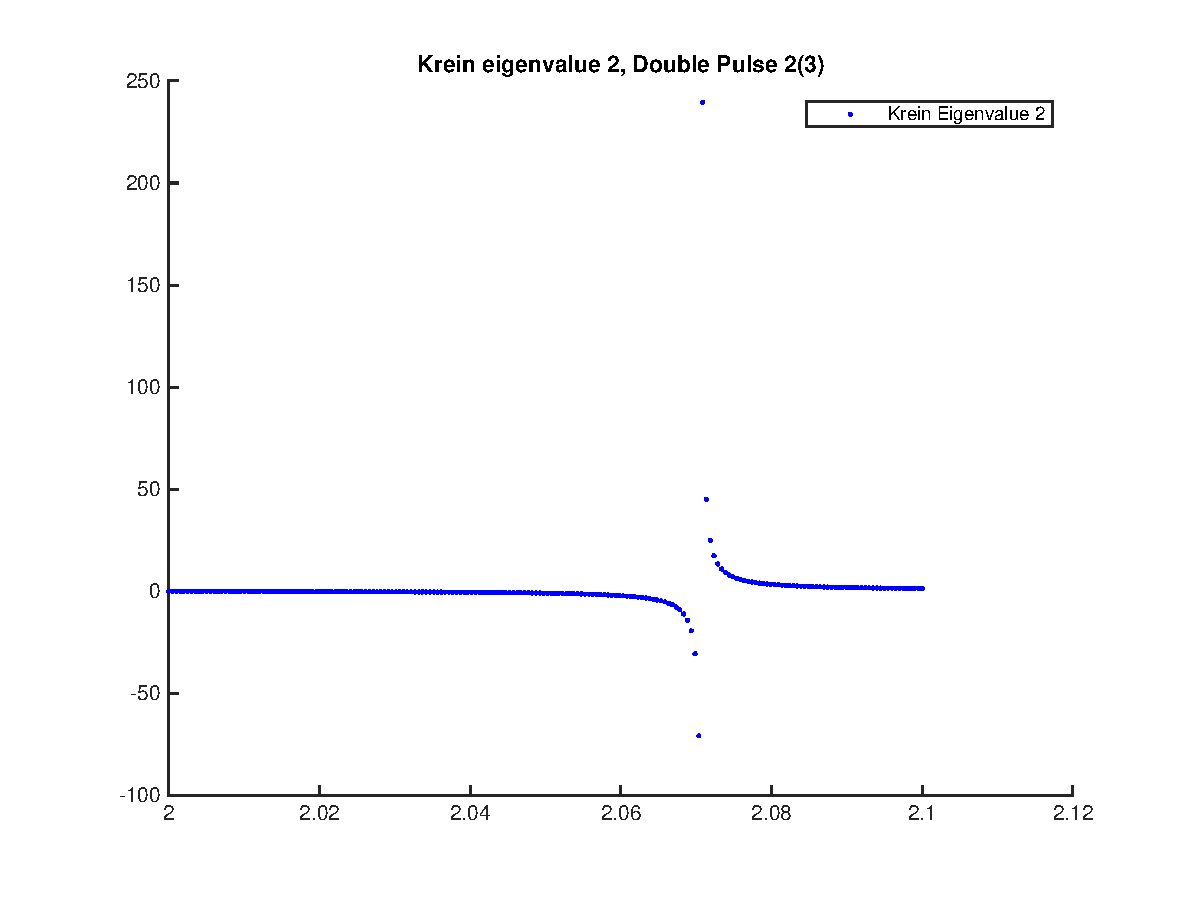
\includegraphics[width=8.5cm]{dp2kreineigzoomsing2.eps}
	\caption{Krein eigenvalue 2, zoom around $z = 2$. Double pulse 2(3), $c = 10$, Fourier spectral methods, $N =  256$, $L = 50$. }
\end{figure}

The curve for Krein eigenvalue 2 crosses 0 at $z = 2.0063$, which corresponds to the value $\lambda = 1.4164i$, which is the smallest (positive) point on the essential spectrum. Now that we know where this occurs, let's look at both Krein eigenvalues. First let's take a look on the interval $z \in [2.0, 2.1]$

\begin{figure}[H]
	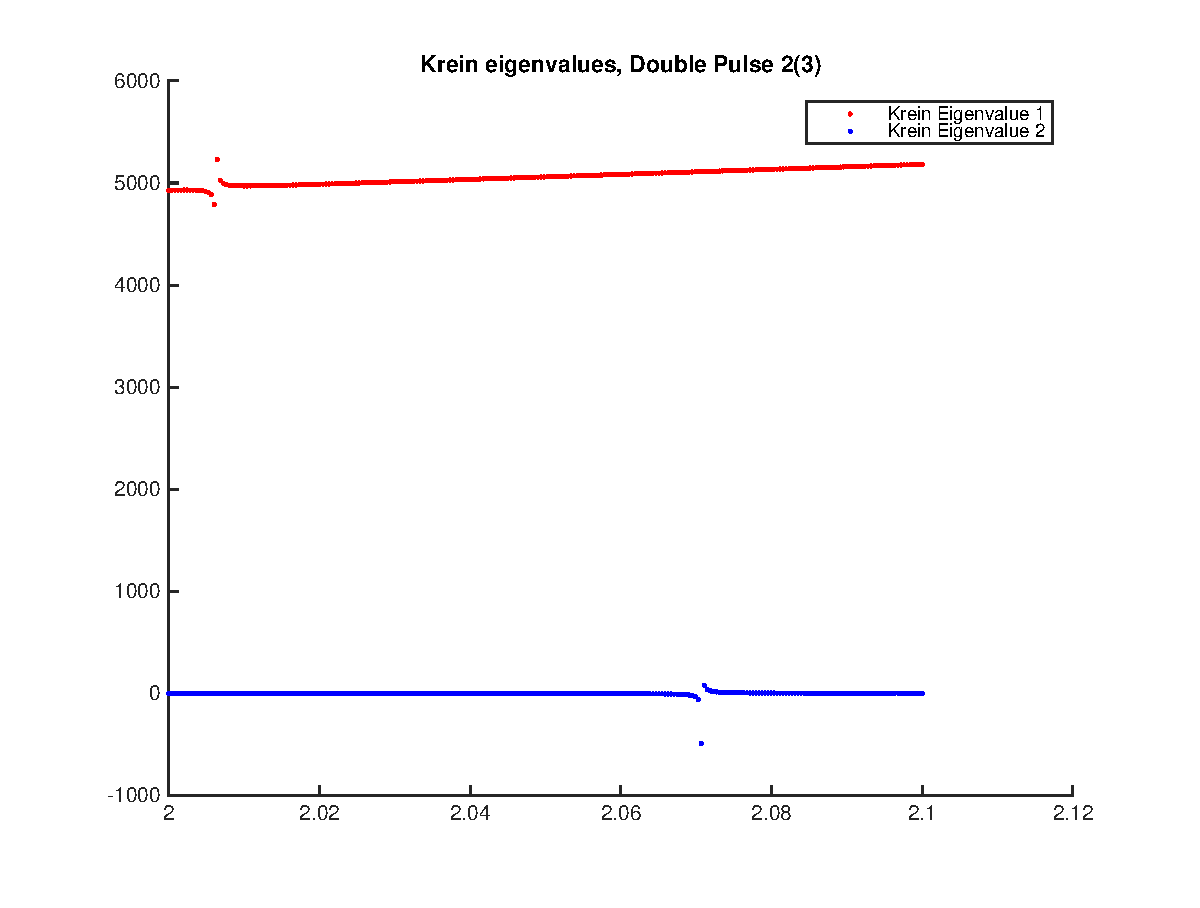
\includegraphics[width=8.5cm]{dp2kreineigsingnear2.eps}
	\caption{Krein eigenvalues 1 and 2, interval $z \in [2.0, 2.1]$, Double pulse 2(3), $c = 10$, Fourier spectral methods, $N = 256$, $L = 50$. }
\end{figure}

Because of the scale on the y-axis, we cannot see the crossing of Krein eigenvalue 2 at $z = 2.0063$. What we can see is a singularity in Krein eigenvalue 2 after this crossing, at about $z = 2.07$. Interestingly, there is also a singularity in Krein eigenvalue 1 which is located right about where Krein eigenvalue 1 crosses 0. Before this singularity, Krein eigenvalue 1 will also cross zero. The question is whether the two crossings are at the same point. To see that, let's zoom in on both eigenvalues right near the crossing at $z = 2.0063$.

\begin{figure}[H]
	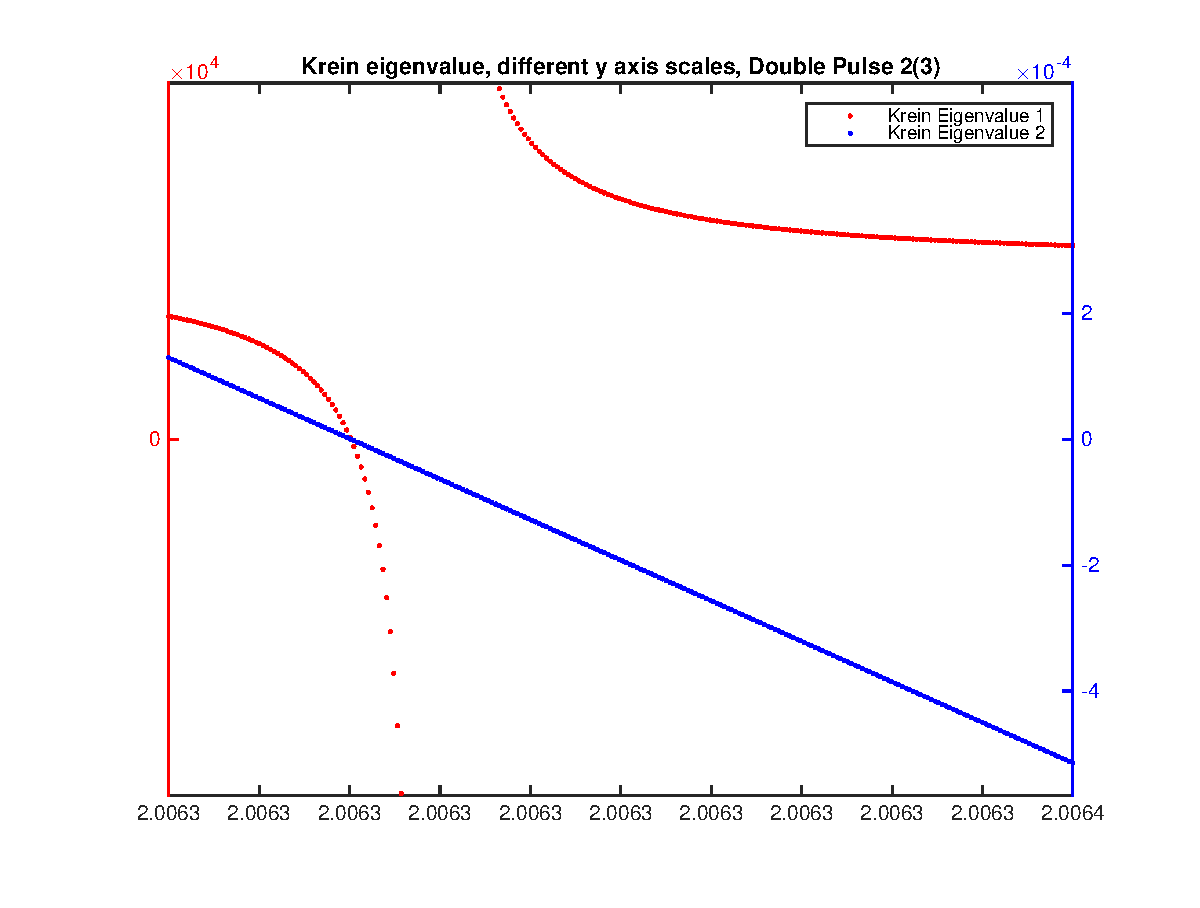
\includegraphics[width=8.5cm]{dp2kreineigsingnear2diffy.eps}
	\caption{Krein eigenvalues 1 and 2, zoom near $z = 2.0063$, different scales on $y$-axis for the two Krein eigenvalues, Double pulse 2(3), $c = 10$, Fourier spectral methods, $N = 256$, $L = 50$. }
\end{figure}

The scales on the two $y$-axes are wildly different, but the plot plus a numerical computation of the intersection of the two curves suggest that they intersect each other and zero at this crossing point, just like we had for the interaction eigenvalue. \\

The same holds for the next eigenvalue in the essential spectrum. Looking at a plot of Krein eigenvalue 2 on the interval $z \in [8.1, 8.2]$, we find that the eigenvalue crosses 0 at $z = 8.1556$, which corresponds to $\lambda = 2.8558i$, the next point in the essential spectrum.

\begin{figure}[H]
	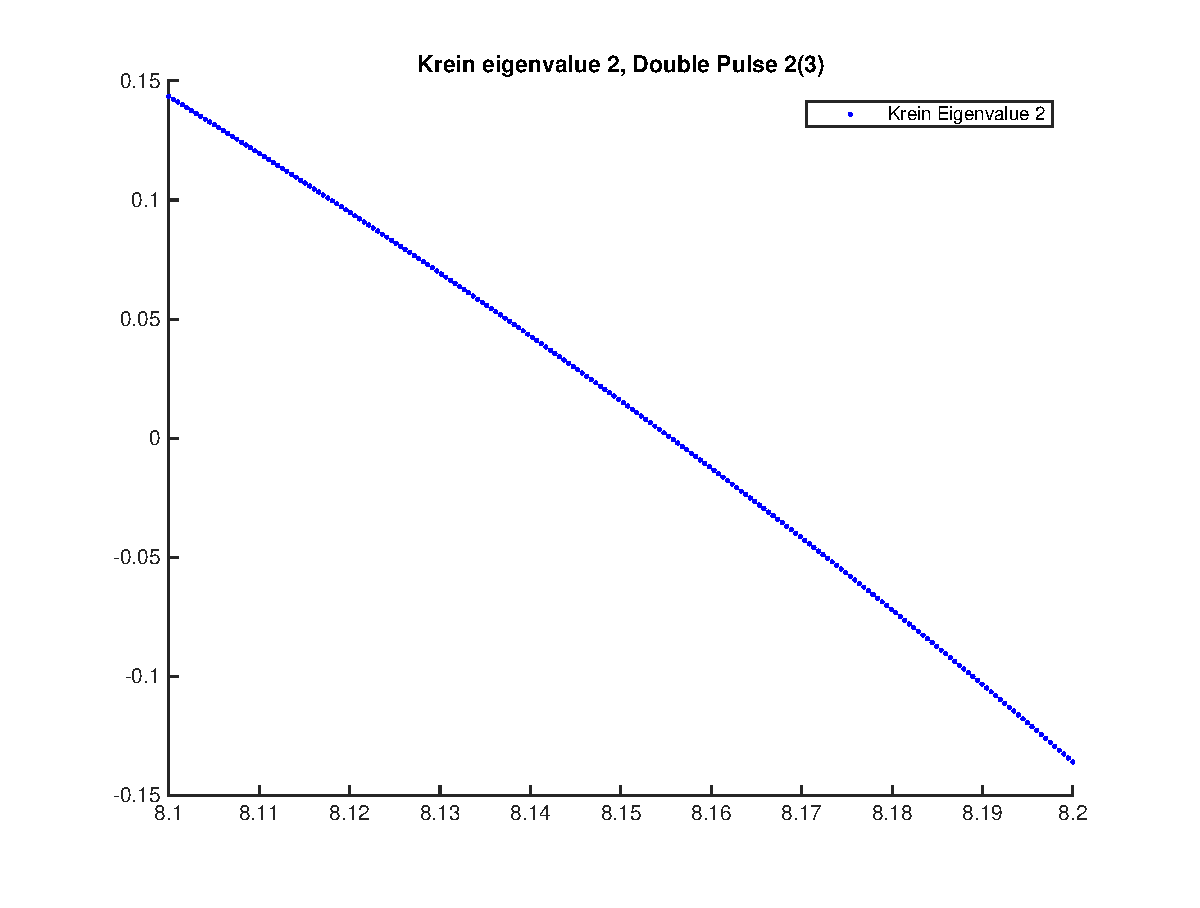
\includegraphics[width=8.5cm]{dp2kreineigsingnear8.eps}
	\caption{Krein eigenvalue 2, interval $z \in [8.1, 8.2]$, different scales on $y$-axis for the two Krein eigenvalues, Double pulse 2(3), $c = 10$, Fourier spectral methods, $N = 256$, $L = 50$. }
\end{figure}

If we zoom in on the crossing at $z = 8.1556$ and use different $y$-axis scales for the two Krein eigenvalues, we get a similar plot as with the first point on the essential spectrum. This plus a numerical computation of the intersection of the curves suggests that the two curves intersect each other and zero at this crossing point.

\begin{figure}[H]
	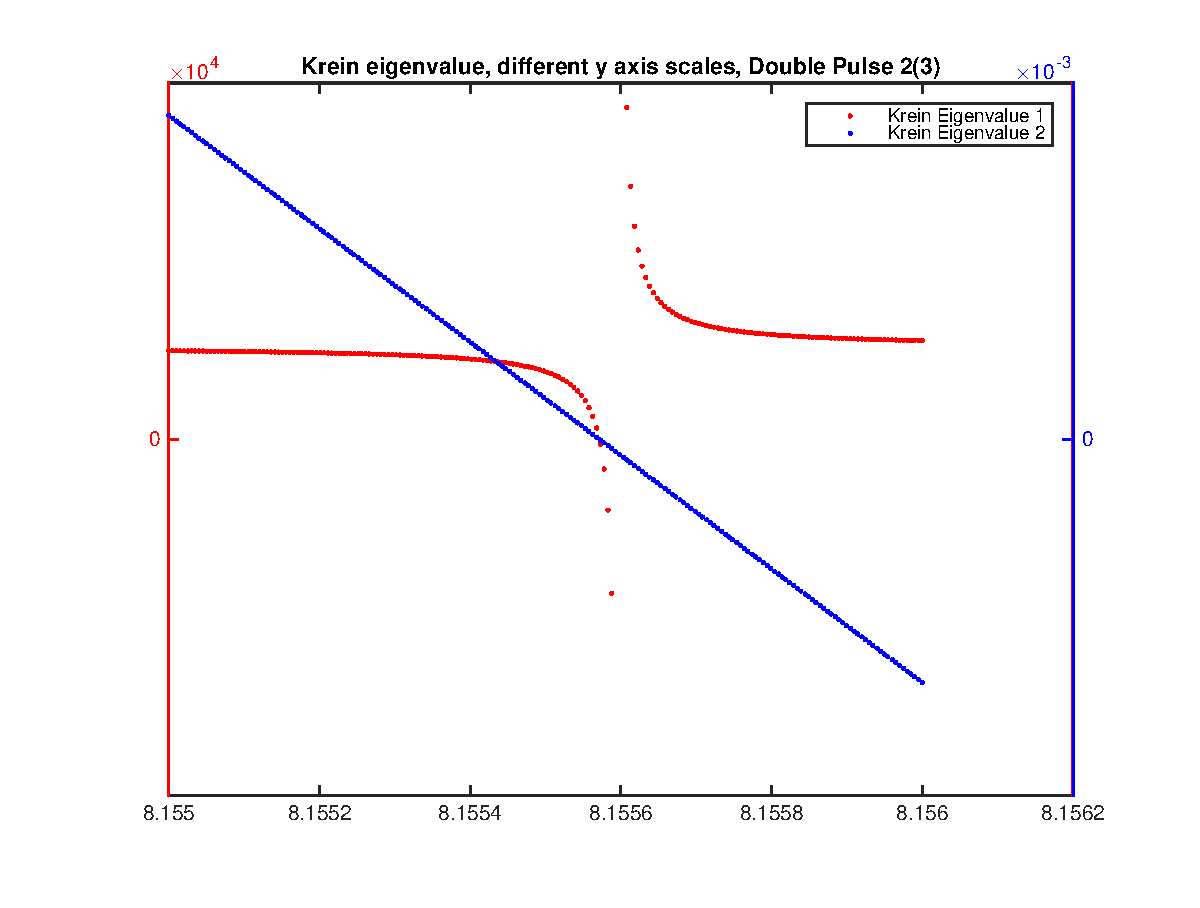
\includegraphics[width=8.5cm]{dp2kreineigsingnear8diffy.eps}
	\caption{Krein eigenvalues 1 and 2, zoom near $z = 8.1556$, different scales on $y$-axis for the two Krein eigenvalues, Double pulse 2(3), $c = 10$, Fourier spectral methods, $N = 256$, $L = 50$. }
\end{figure}

Putting this all together, we can make a badly drawn cartoon. Note that the zeros of the two Krein eigenvalue curves coincide, but the singularities do not. The singularity for Krein eigenvalue 1 occurs before the singularity for Krein eigenvalue 2, at least as far as we have gone with the plot.

\begin{figure}[H]
	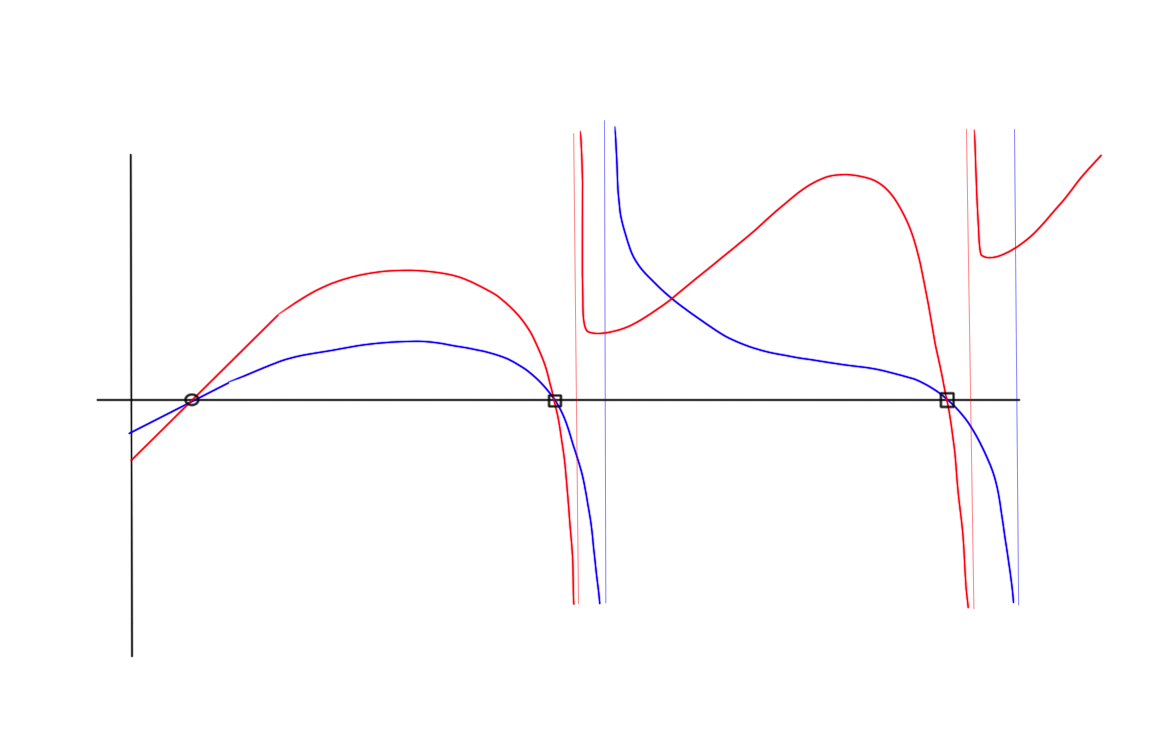
\includegraphics[width=15cm]{kreineigcartoon3.png}
	\caption{Cartoon of Krein eigenvalues. Red is Krein eigenvalue 1, Blue is Krein eigenvalue 2. Intersections are on the x-axis, as we showed numerically above. Black circle is interaction eigenvalue, which has negative Krein signature, maybe because slopes of both eigenvalue lines are positive? (this is consistent with Kapitula). Black squares are the first two essential spectrum eigenvalues, which have positive Krein signature (slopes of both eigenvalue lines are negative.}
\end{figure}

It would be useful to repeat this for the case were the interaction eigenvalue and the smallest essential spectrum eigenvalue cross. From what we showed before, this does not produce a Krein collision, although we would normally expect one to occur at the crossing. As we did when we looked at the crossing, we use double pulse 2(3), $c = 150$, Fourier spectral methods, $N = 1024$. The interaction eigenvalues is independent of domain length, while the location of the essential spectrum eigenvalues depends on domain length.\\

First, consider the domain length $L = 115$. For these parameters, we found previously that the interaction eigenvalue is $3.9859i$, and the first two eigenvalues of the essential spectrum of $4.1454i$ and $8.2914i$.

\begin{figure}[H]
	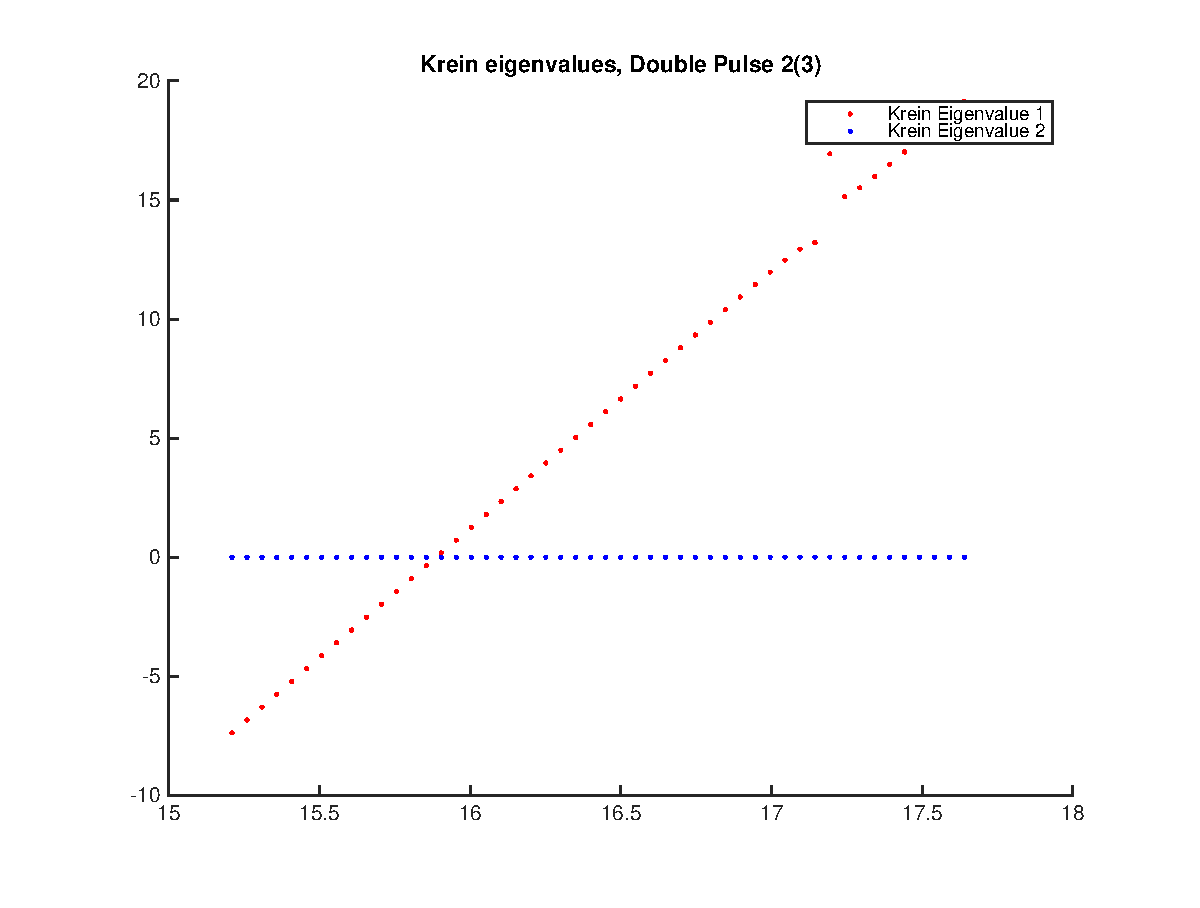
\includegraphics[width=8.5cm]{1500F_dp2_115_krein1.eps}
	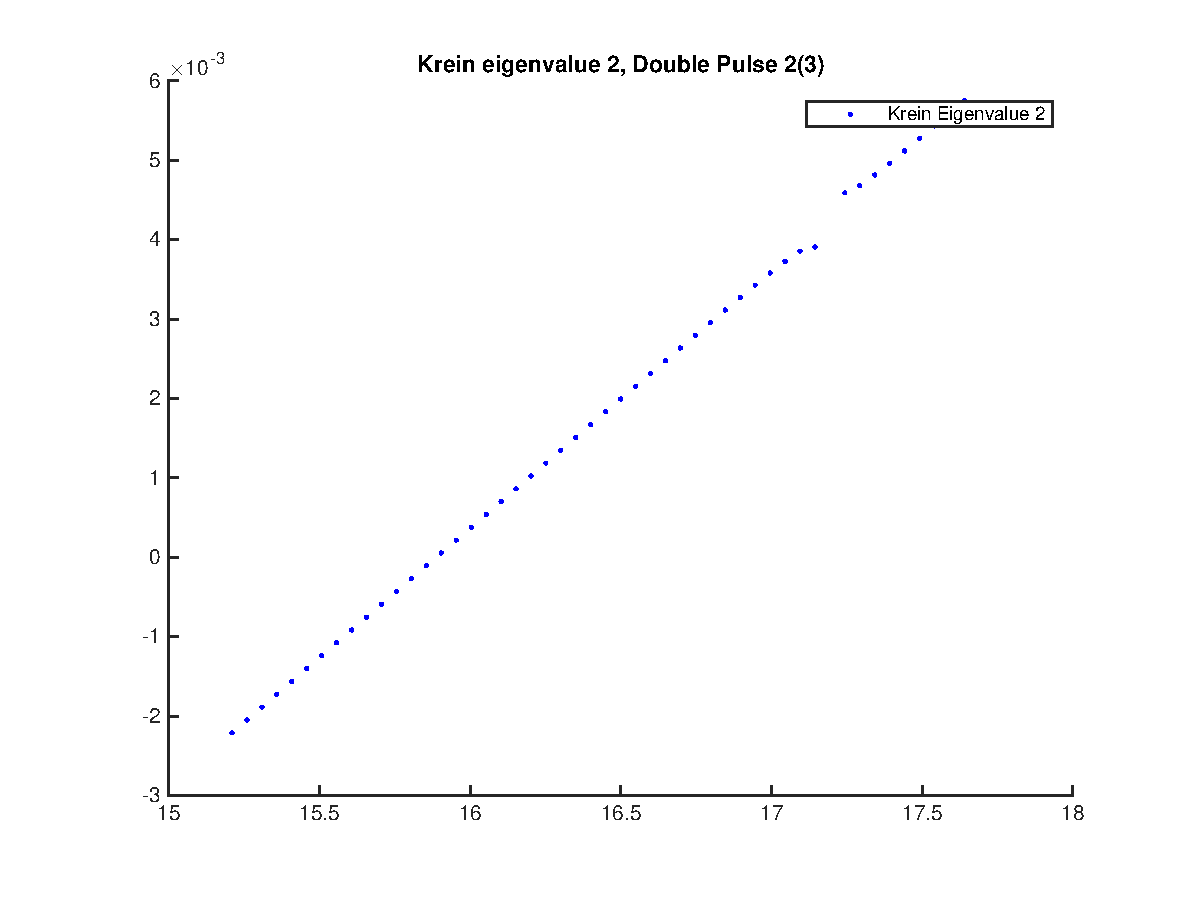
\includegraphics[width=8.5cm]{1500F_dp2_115_krein2.eps}
	\caption{Krein eigenvalues 1 and 2 (left) and Krein eigenvalue 2 (right), interval $z \in [15, 24]$, double pulse 2(3), $c = 150$, Fourier spectral methods, $N = 1024$, $L = 115$. }
\end{figure}

The two Krein eigenvalues lines cross each other and zero at $z = 15.8875$, which corresponds to $\lambda = 3.9859i$, which is the interaction eigenvalue. We don't see a crossing for the essential spectrum eigenvalue here, but we see what looks like singularities in the two eigenvalue curves around $z = 17$, so we will look there. We also expect the first essential spectrum eigenvalue to correspond to $z = 17.1843$.

\begin{figure}[H]
	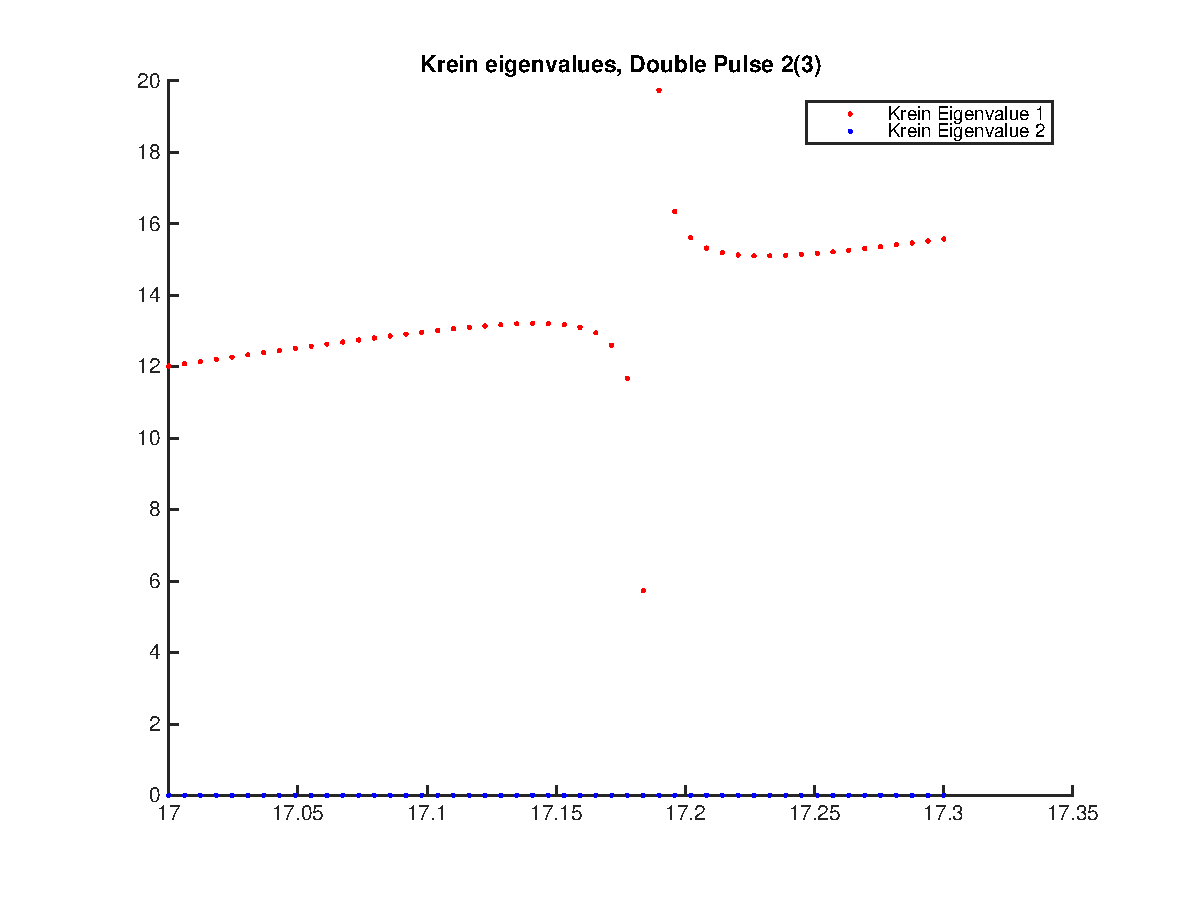
\includegraphics[width=8.5cm]{1500F_dp2_115_kreinzoom1.eps}
	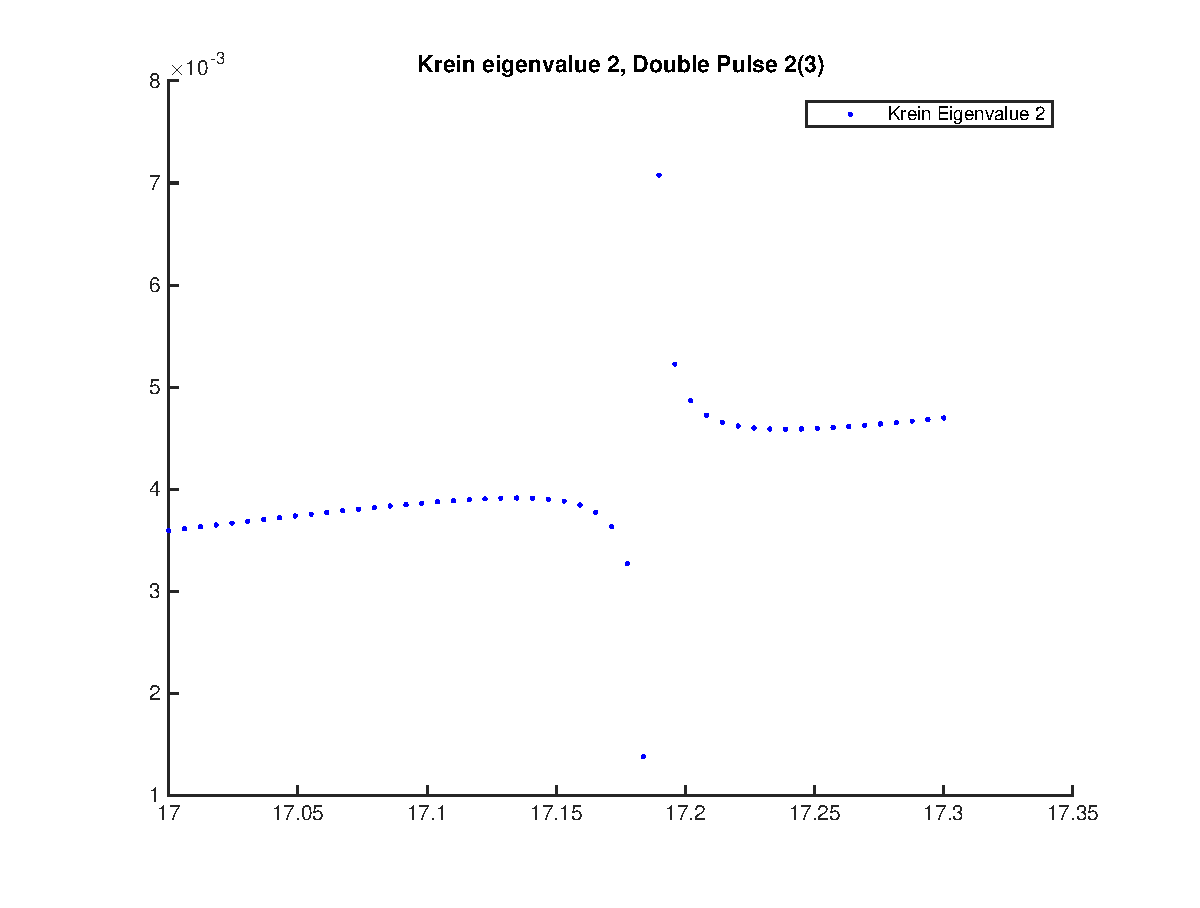
\includegraphics[width=8.5cm]{1500F_dp2_115_kreinzoom2}
	\caption{Krein eigenvalues 1 and 2 (left) and Krein eigenvalue 2 (right), interval $z \in [17, 17.3]$, double pulse 2(3), $c = 150$, Fourier spectral methods, $N = 1024$, $L = 115$. }
\end{figure}

Zooming into the interval $z \in [17, 17.3]$, we see both eigenfunctions will have singularities around $z = 17.18$, but we cannot yet see the crossing of zero. More zoom is needed. (As for why we didn't start by taking a finer mesh, we are inverting a 1024x1024 matrix each time we compute the Krein matrix, and that is slow.) Finally, we zoom in on the interval $z \in [17.18, 17.19]$.

\begin{figure}[H]
	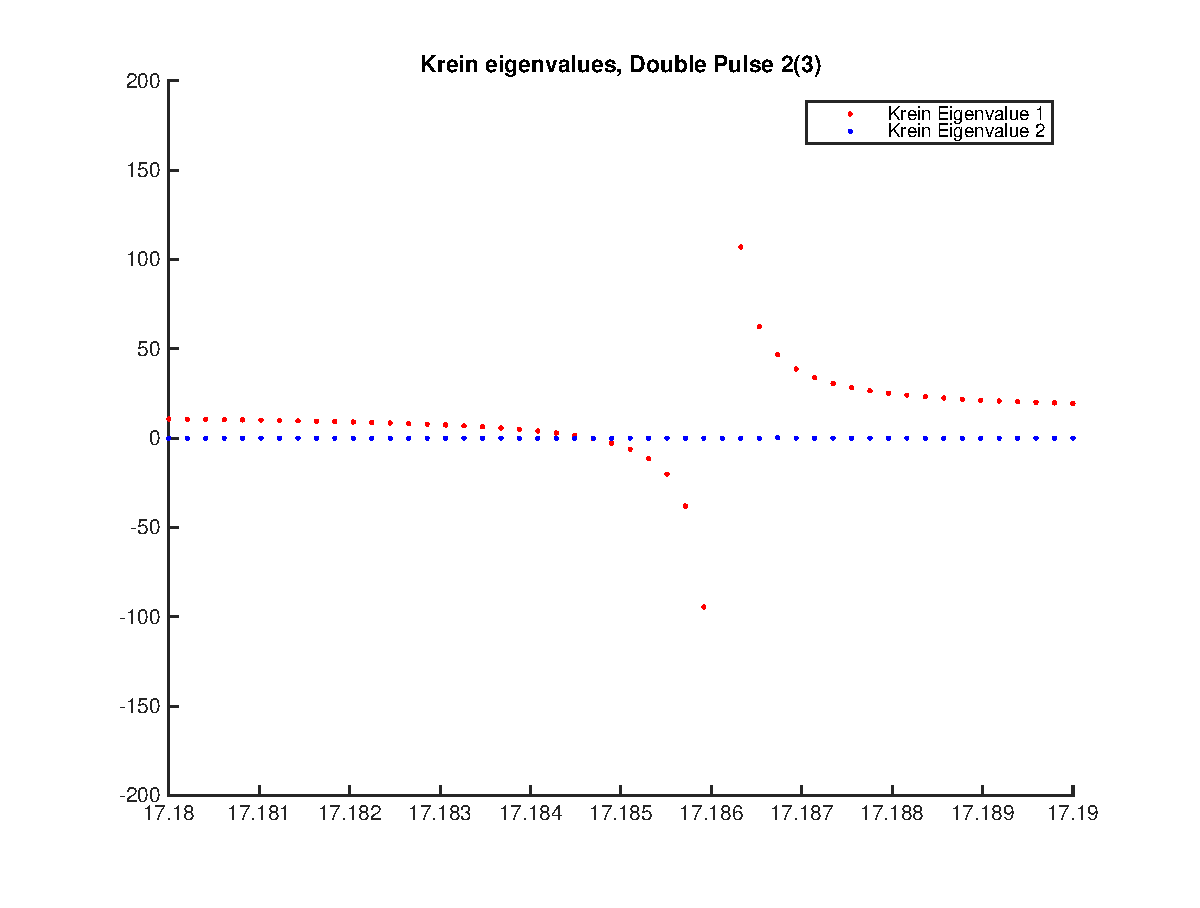
\includegraphics[width=8.5cm]{1500F_dp2_115_kreinzoom3.eps}
	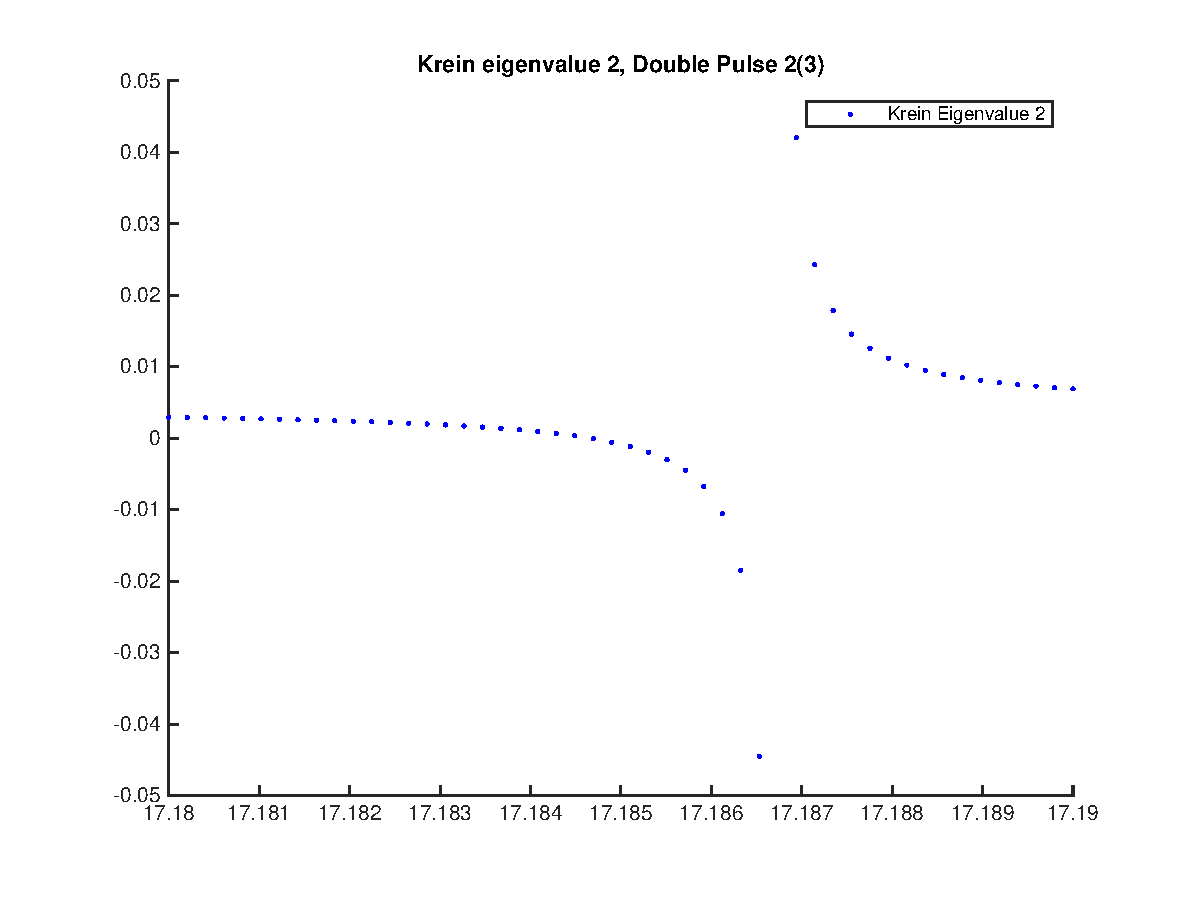
\includegraphics[width=8.5cm]{1500F_dp2_115_kreinzoom4}
	\caption{Krein eigenvalues 1 and 2 (left) and Krein eigenvalue 2 (right), interval $z \in [17.18, 17.19]$, double pulse 2(3), $c = 150$, Fourier spectral methods, $N = 1024$, $L = 115$. }
\end{figure}

We see both crossings here of zero, and can compute numerically that the two Krein eigenvalue curves cross each other and zero at $z = 17.1847$, which corresponds to $\lambda = 4.1454i$, the first point on the essential spectrum. We also can see the two singularities, and it looks like the singularity for Krein eigenvalue 1 occurs before that of Krein eigenvalue 2, which is what we observed before.\\

All of this is exactly as we expect, i.e. no different from the earlier case, since the crossing has not yet occurred. We have another badly drawn cartoon for this, which looks like the previous one.

\begin{figure}[H]
	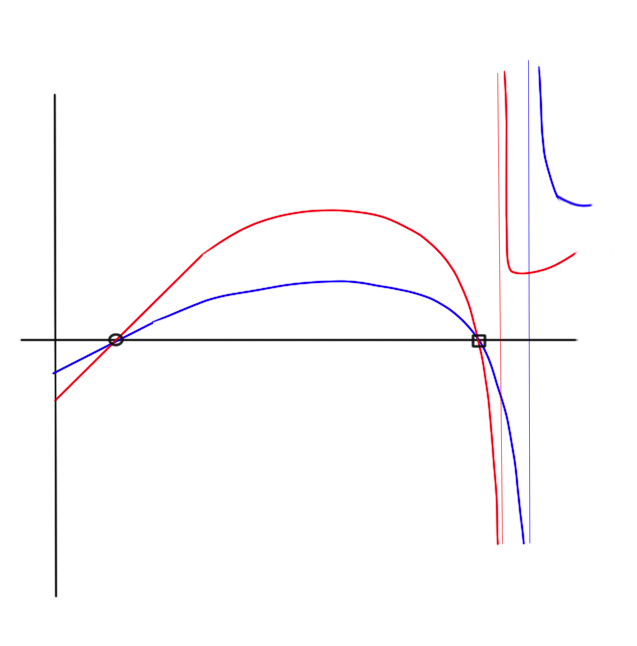
\includegraphics[width=15cm]{kreincartoonbeforecrossing.png}
	\caption{Cartoon of Krein eigenvalues (before crossing). Red is Krein eigenvalue 1, Blue is Krein eigenvalue 2. Intersections are on the x-axis, as we showed numerically above. Black circle is interaction eigenvalue, which has negative Krein signature. Black square is the first essential spectrum eigenvalues, which has positive Krein signature. Double pulse 2(3), $c = 150$, Fourier spectral methods, $N = 1024$, $L = 115$.}
\end{figure}

Now let's look after the crossing. $L = 125$ is after that, so we will use that domain length. The rest of the parameters will be the same. For these parameters, we found previously that the interaction eigenvalue is $3.9859i$ (unchanged, as expected), and the first eigenvalue of the essential spectrum is $3.8106i$, which is below the interaction eigenvalue on the imaginary axis. First, we look at the interval $z \in [14, 16]$.

\begin{figure}[H]
	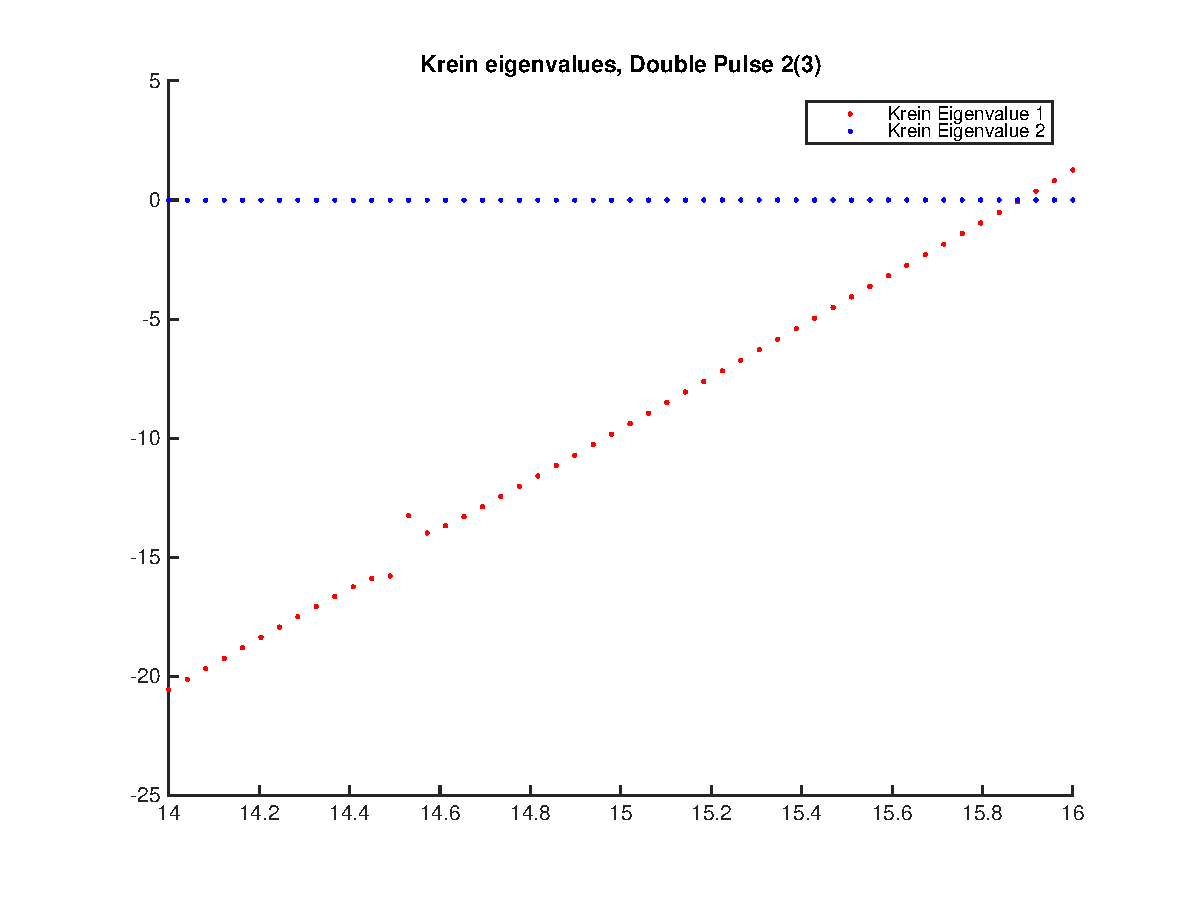
\includegraphics[width=8.5cm]{1500F_dp2_125_krein1.eps}
	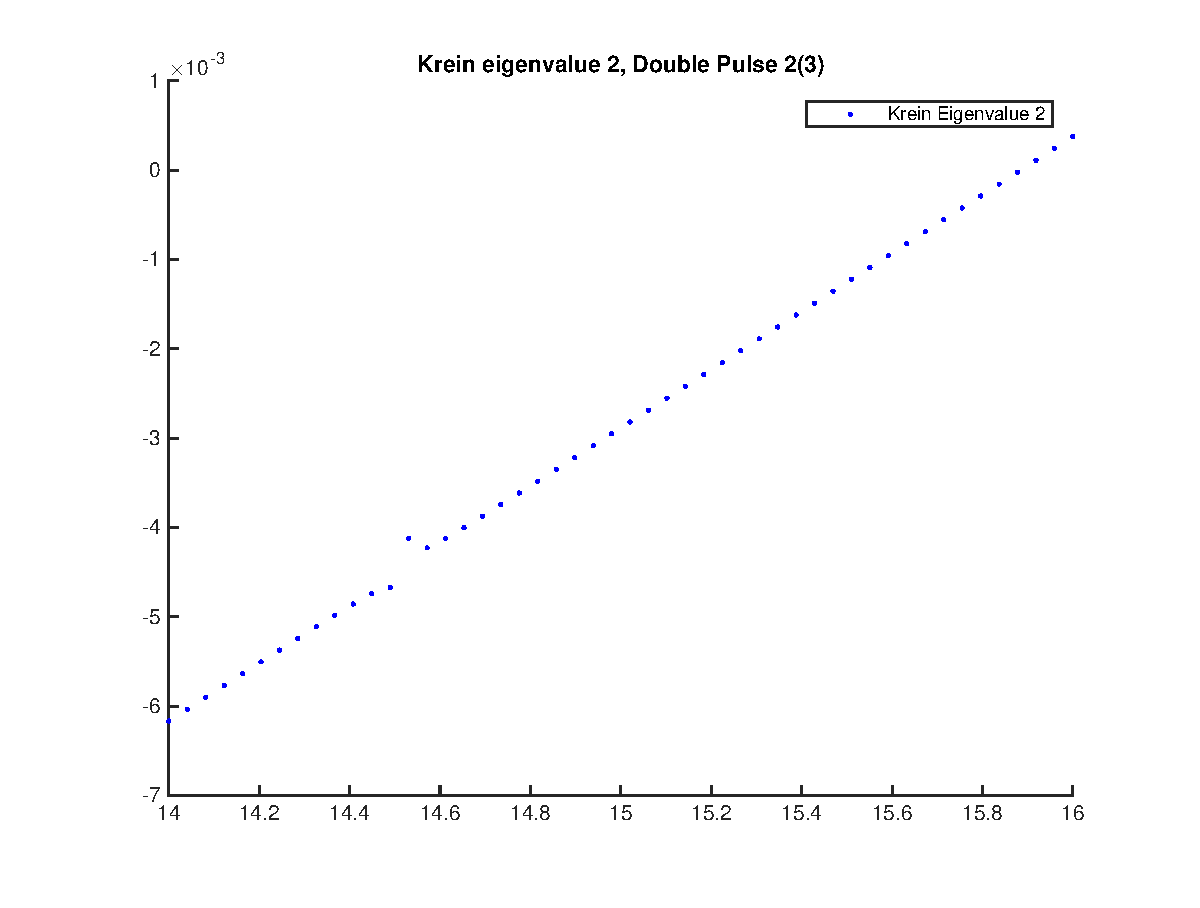
\includegraphics[width=8.5cm]{1500F_dp2_125_krein2.eps}
	\caption{Krein eigenvalues 1 and 2 (left) and Krein eigenvalue 2 (right), interval $z \in [14, 16]$, double pulse 2(3), $c = 150$, Fourier spectral methods, $N = 1024$, $L = 125$. }
\end{figure}

On the right side, we see the crossing around $z = 15.8$ which will correspond to the interaction eigenvalue. On the left, we see the singularities around which we will have the crossing corresponding to the essential spectrum eigenvalue. We can basically see what is going to happen from this alone, but for completeness we will zoom in on the relevant regions. First we locate the interaction eigenvalue by looking at the interval $z \in [15.8, 15.9]$. We see the two Krein eigenvalue curves cross each other and zero at $z = 15.8844$, corresponding to $\lambda = 3.9855i$, which is really close to the interaction eigenvalue we found before.

\begin{figure}[H]
	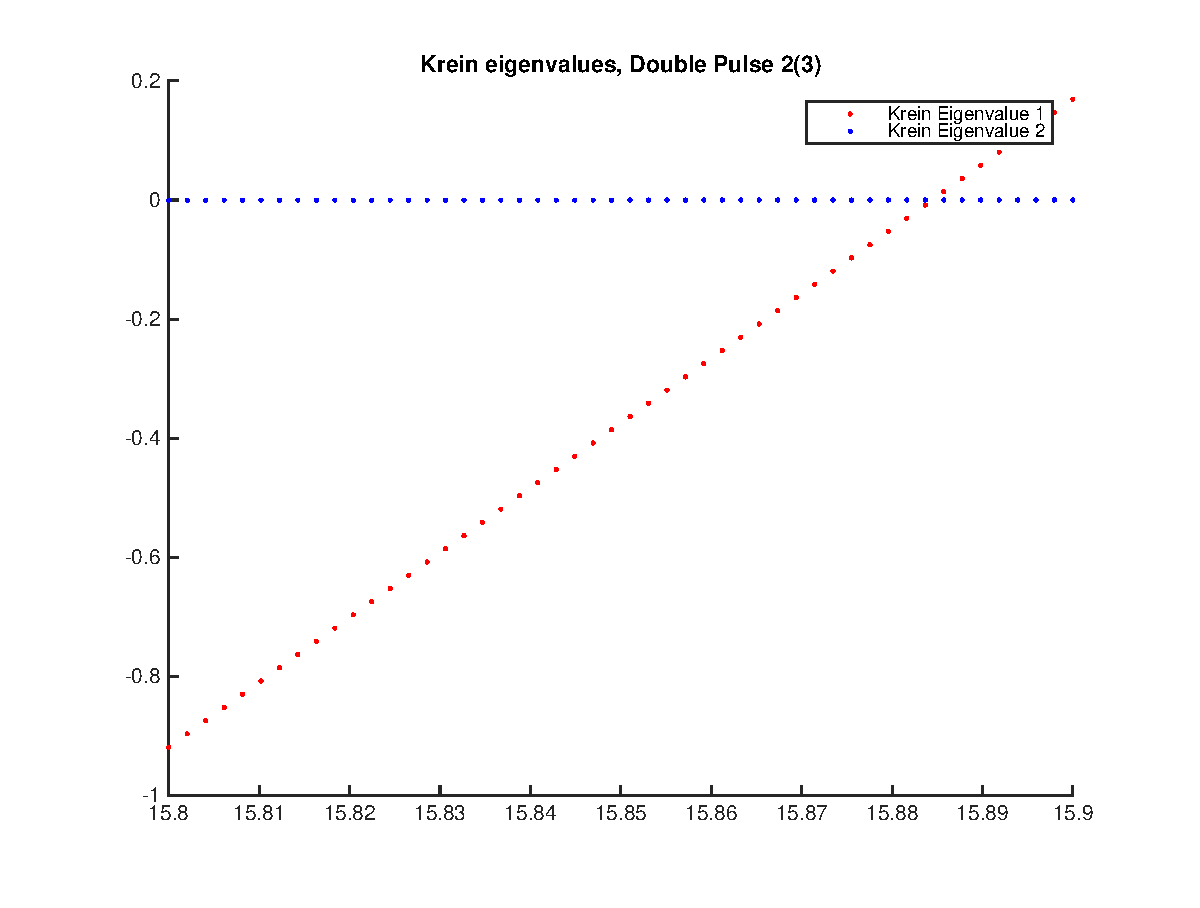
\includegraphics[width=8.5cm]{1500F_dp2_125_kreinzoom1.eps}
	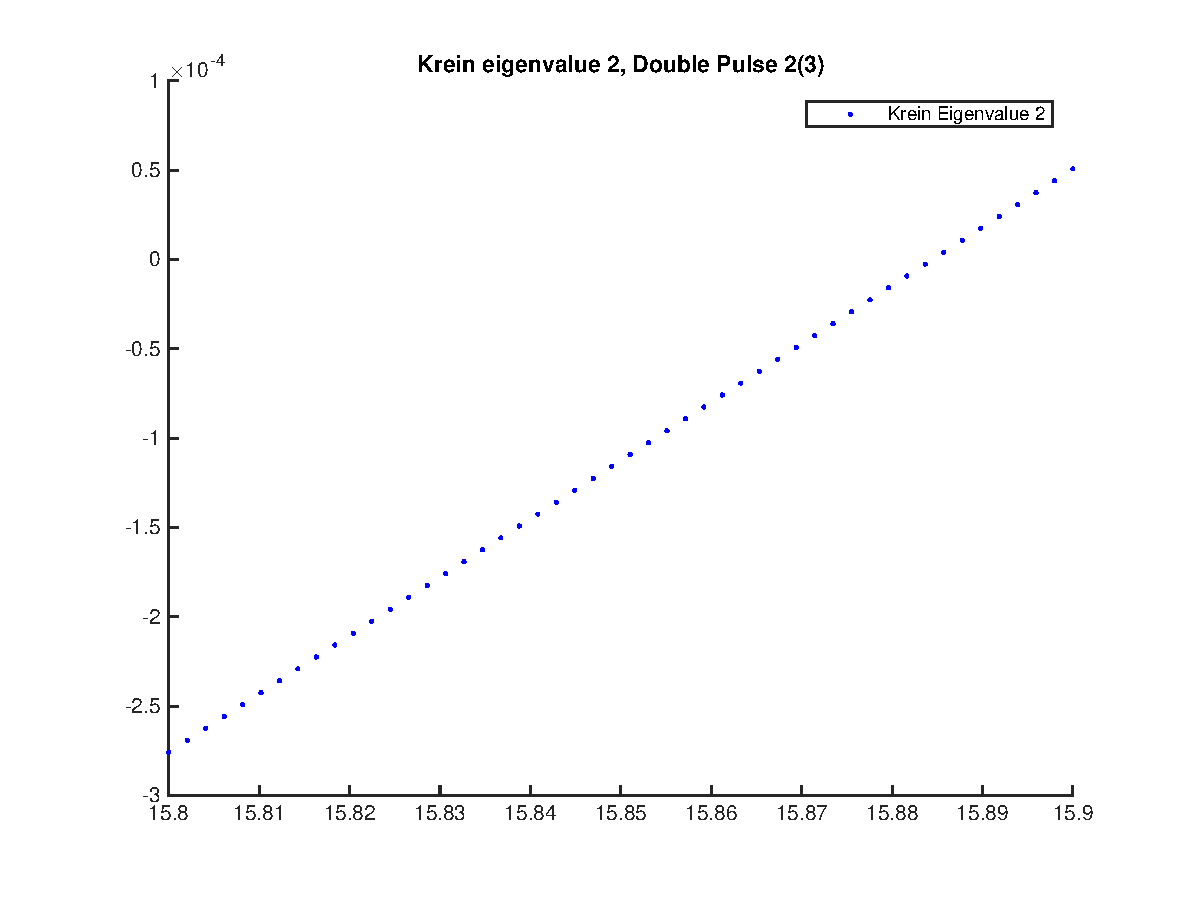
\includegraphics[width=8.5cm]{1500F_dp2_125_kreinzoom2.eps}
	\caption{Krein eigenvalues 1 and 2 (left) and Krein eigenvalue 2 (right), interval $z \in [15.8, 15.9]$, double pulse 2(3), $c = 150$, Fourier spectral methods, $N = 1024$, $L = 125$. }
\end{figure}

Now we try to see what is happening near the essential spectrum eigenvalue. Looking at the interval $z \in [14.5, 14.6]$ we see that what will happen here is that the right side of the singularity will shoot down and cross zero from above. The plots below show that it is what is going to happen, but we don't yet have enough zoom to see it happen.

\begin{figure}[H]
	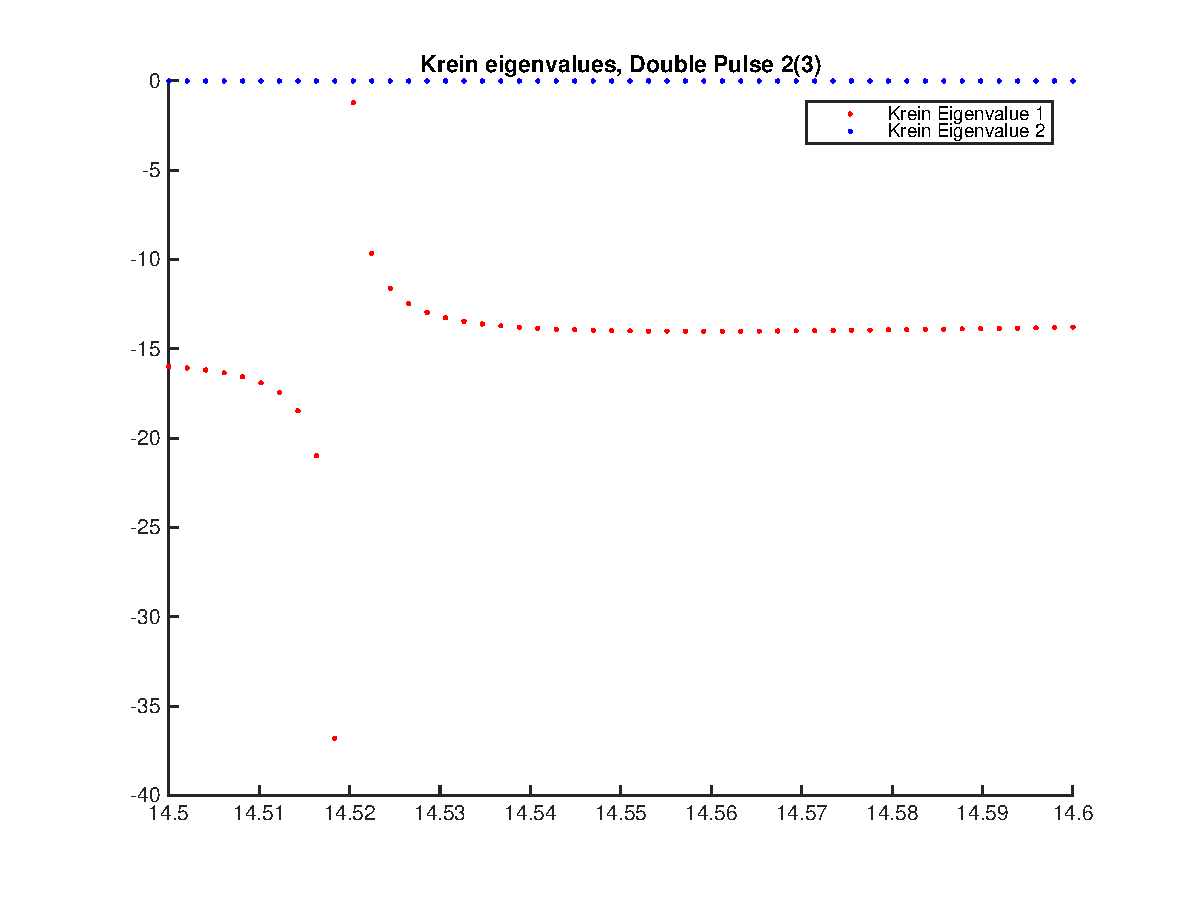
\includegraphics[width=8.5cm]{1500F_dp2_125_kreinzoom3.eps}
	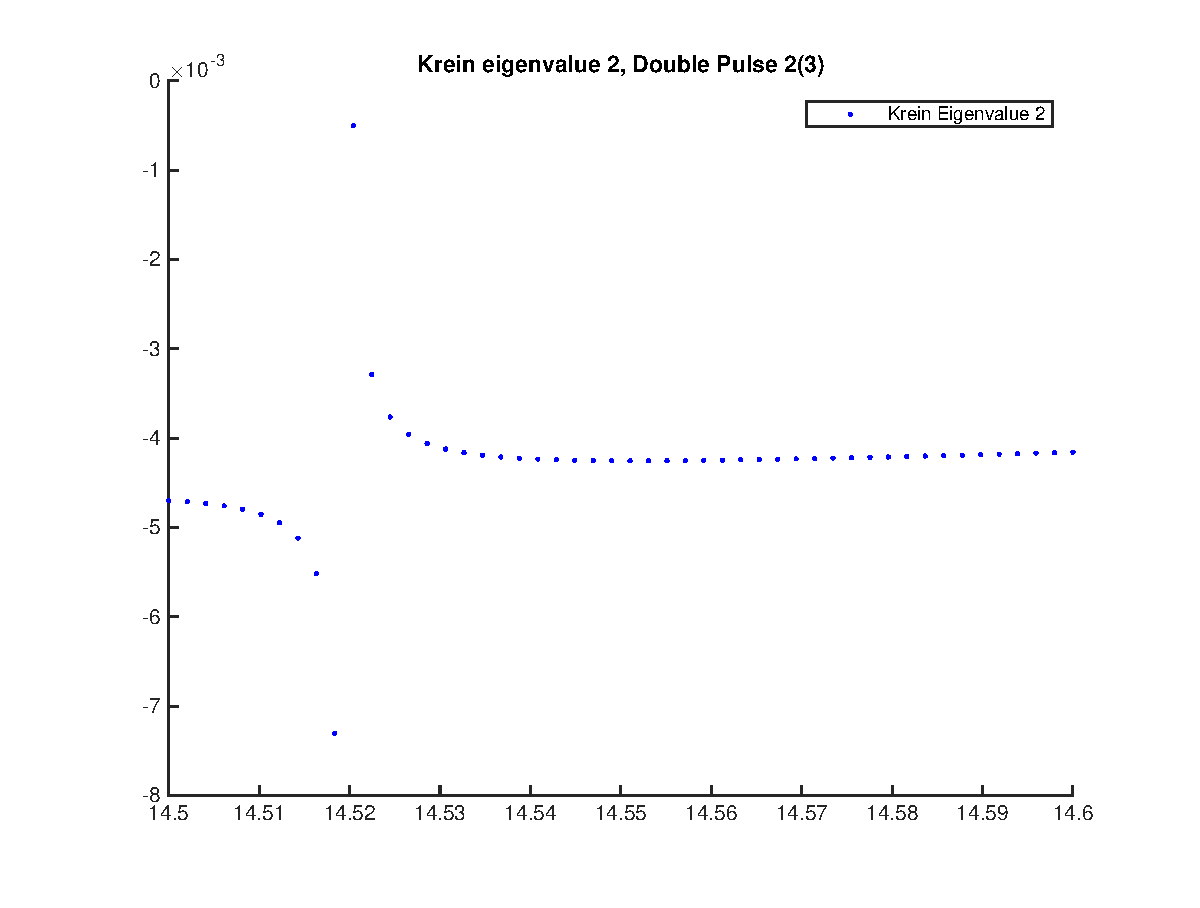
\includegraphics[width=8.5cm]{1500F_dp2_125_kreinzoom4.eps}
	\caption{Krein eigenvalues 1 and 2 (left) and Krein eigenvalue 2 (right), interval $z \in [15.8, 15.9]$, double pulse 2(3), $c = 150$, Fourier spectral methods, $N = 1024$, $L = 125$. }
\end{figure}

If we zoom in on the interval $z \in [14.51, 14.53]$, we can see the crossing corresponding to the essential spectrum eigenvalue. This occurs at $z = 14.5203$, which corresponds to the lowest essential spectrum eigenvalue of $\lambda = 3.8106i$. As before, it appears that Krein eigenvalue 1 has a singularity slightly  before that of Krein eigenvalue 2.

\begin{figure}[H]
	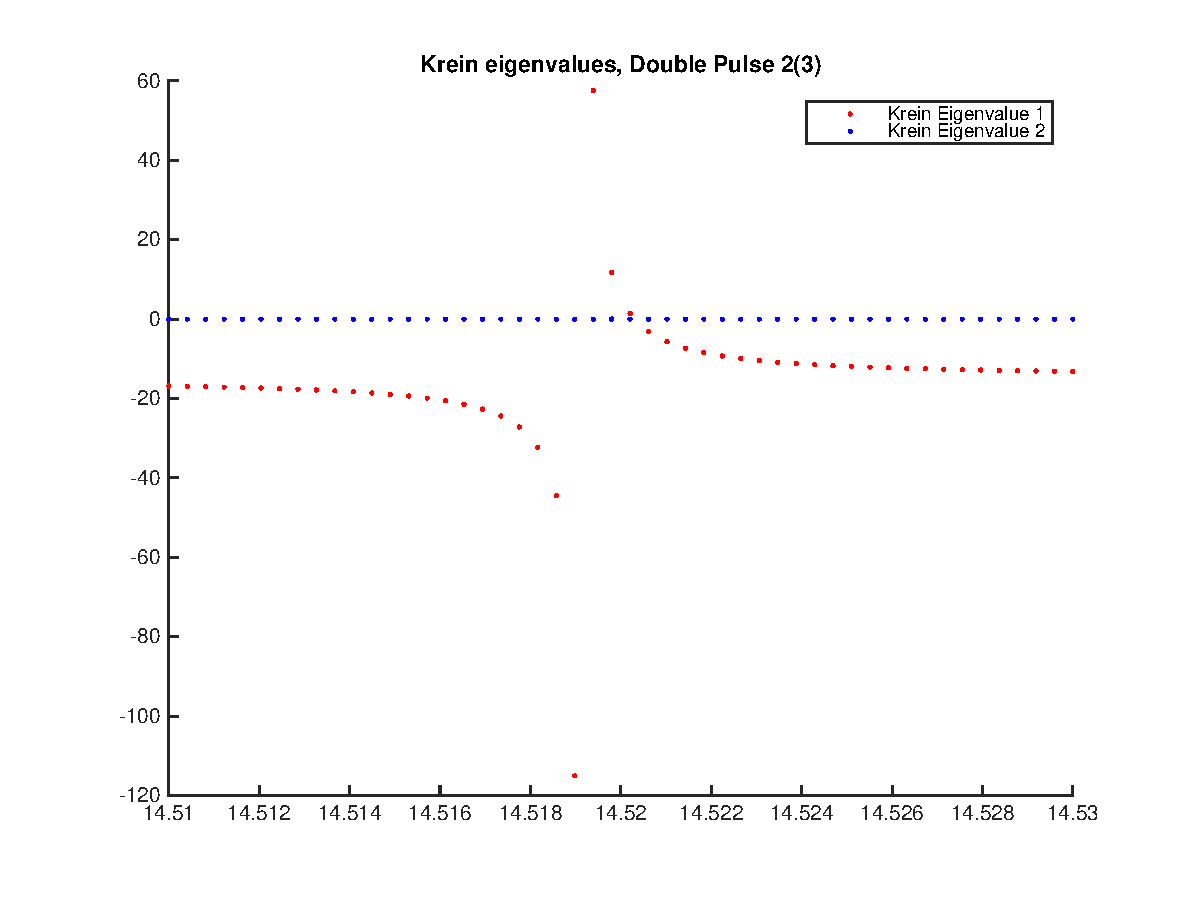
\includegraphics[width=8.5cm]{1500F_dp2_125_kreinzoom5.eps}
	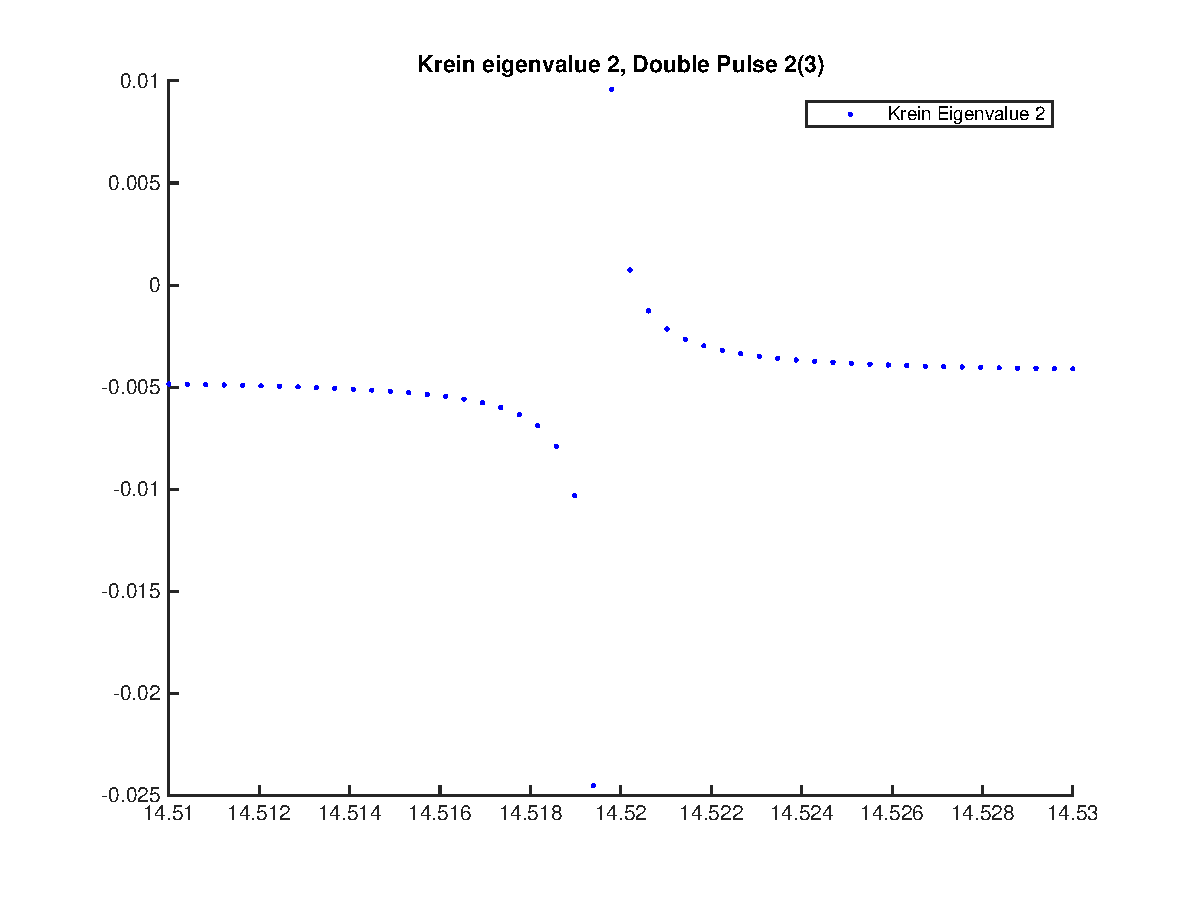
\includegraphics[width=8.5cm]{1500F_dp2_125_kreinzoom6.eps}
	\caption{Krein eigenvalues 1 and 2 (left) and Krein eigenvalue 2 (right), interval $z \in [15.8, 15.9]$, double pulse 2(3), $c = 150$, Fourier spectral methods, $N = 1024$, $L = 125$. }
\end{figure}

We can illustrate this in another badly drawn cartoon. (I did check to make sure the segment between 0 and 14 is correct in the cartoon).

\begin{figure}[H]
	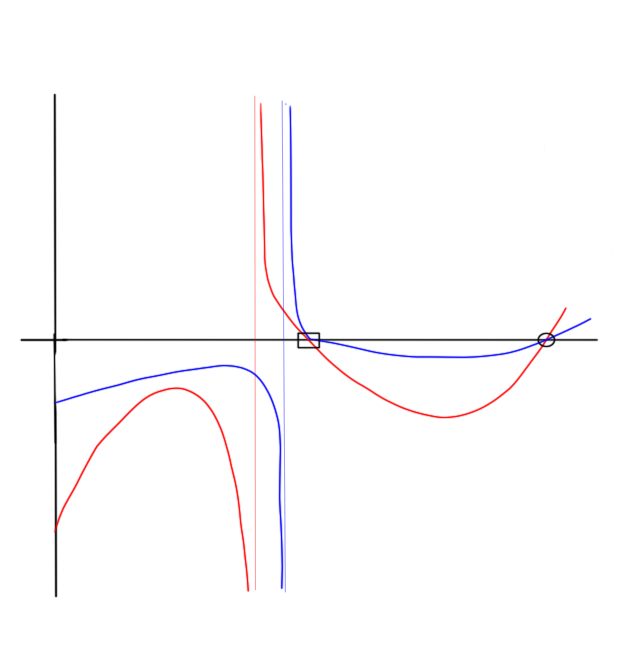
\includegraphics[width=15cm]{kreincartoonaftercrossing.png}
	\caption{Cartoon of Krein eigenvalues (after crossing). Red is Krein eigenvalue 1, Blue is Krein eigenvalue 2. Intersections are on the x-axis, as we showed numerically above. Black circle is interaction eigenvalue, which has negative Krein signature. Black square is the first essential spectrum eigenvalues, which has positive Krein signature. Double pulse 2(3), $c = 150$, Fourier spectral methods, $N = 1024$, $L = 125$.}
\end{figure}

We can get a good picture just after the Krein crossing. For $L = 120$, the essential spectrum eigenvalue is $3.9731i$ and the interaction eigenvalue is $3.9835i$. We can see the two curves crossing each other and zero at both of these points. Note that as in the other cases, the singularity in Krein eigenvalue 1 appears before that of Krein eigenvalue 2 (we can see where this happens on the left of the plot).

\begin{figure}[H]
	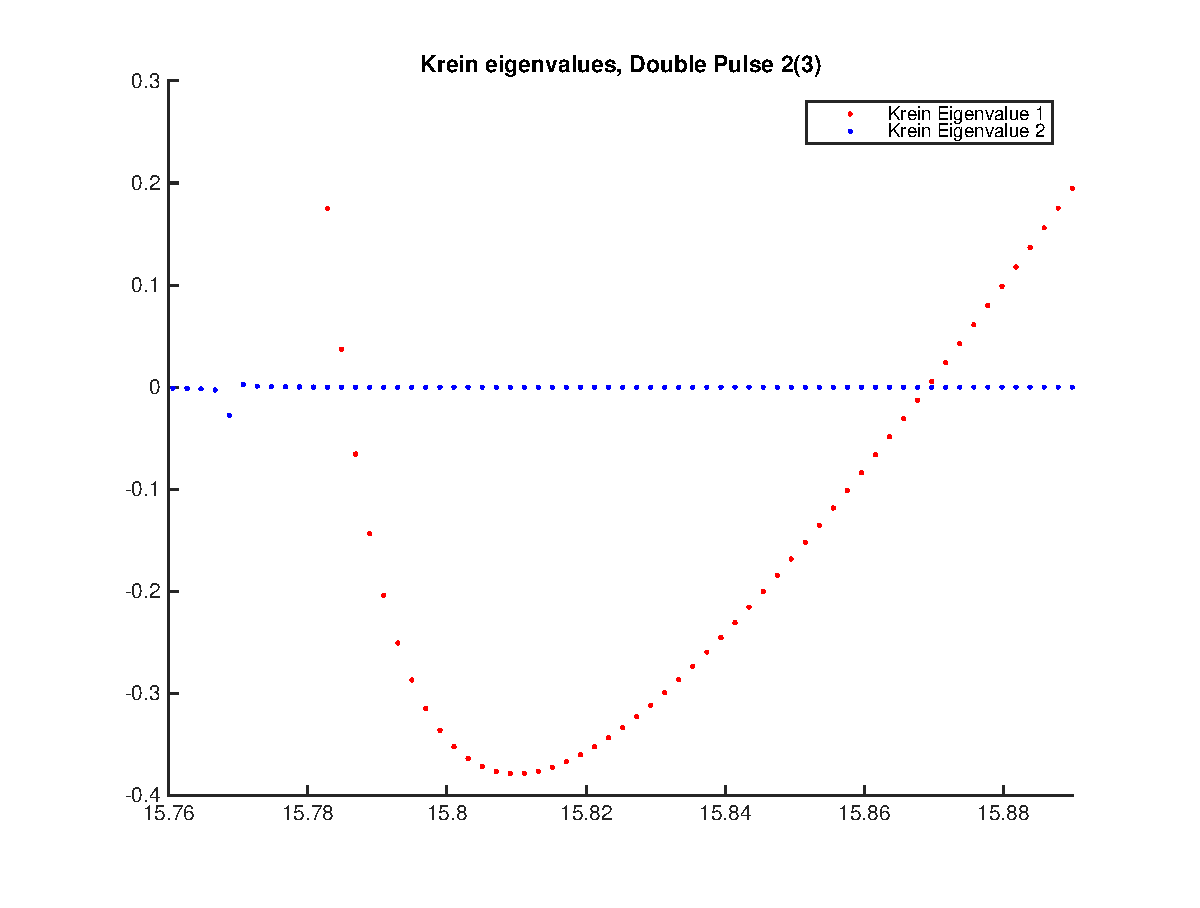
\includegraphics[width=8.5cm]{1500F_dp2_120_krein1.eps}
	\caption{Krein eigenvalues 1 and 2 (left) and Krein eigenvalue 2 (right), double pulse 2(3), $c = 150$, Fourier spectral methods, $N = 1024$, $L = 120$. }
\end{figure}

We can also get a good picture just before the Krein crossing. For $L = 119$, the essential spectrum eigenvalue is $4.0032i$ and the interaction eigenvalue is $3.9870i$. Here is the plot of the two Krein eigenvalue curves for that case.

\begin{figure}[H]
	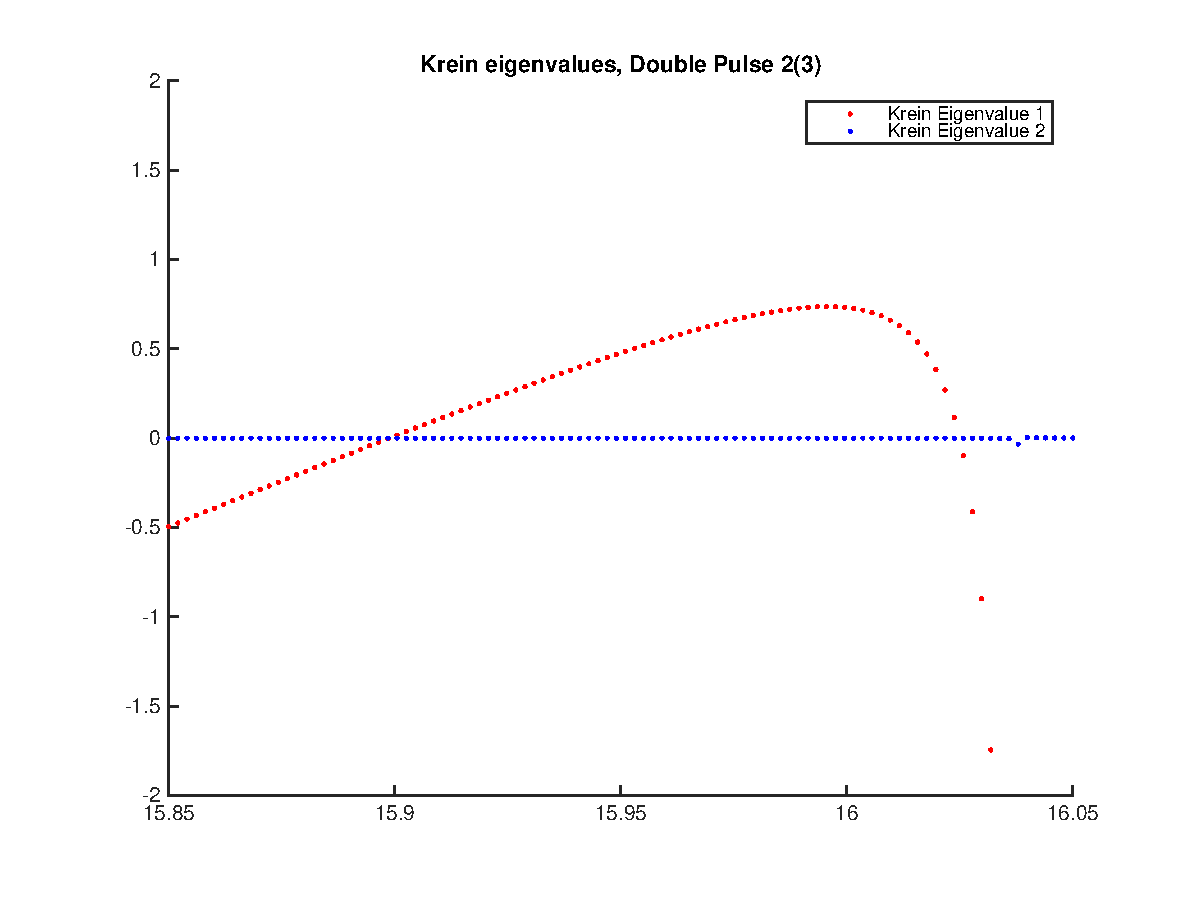
\includegraphics[width=8.5cm]{1500F_dp2_119_krein1.eps}
	\caption{Krein eigenvalues 1 and 2 (left) and Krein eigenvalue 2 (right), double pulse 2(3), $c = 150$, Fourier spectral methods, $N = 1024$, $L = 119$. }
\end{figure}

\section*{Potential Krein Collision}

I am not sure I believe any of these numerics, but I have left this in here anyway.\\

We would like to see what happens exactly at the Krein crossing, so we need to essentially split the difference between the above. Let's try $L = 119.5$. Using Matlab's \texttt{eig}, we have a Krein quartet of eigenvalues at $\pm0.0050 \pm 3.9867i$. The question is whether or not we believe this, since the domain size is huge relative to the width of the double pulse. For now, let's run with it and see what happens. First, we can look at the corresponding eigenfunctions. 

\begin{figure}[H]
	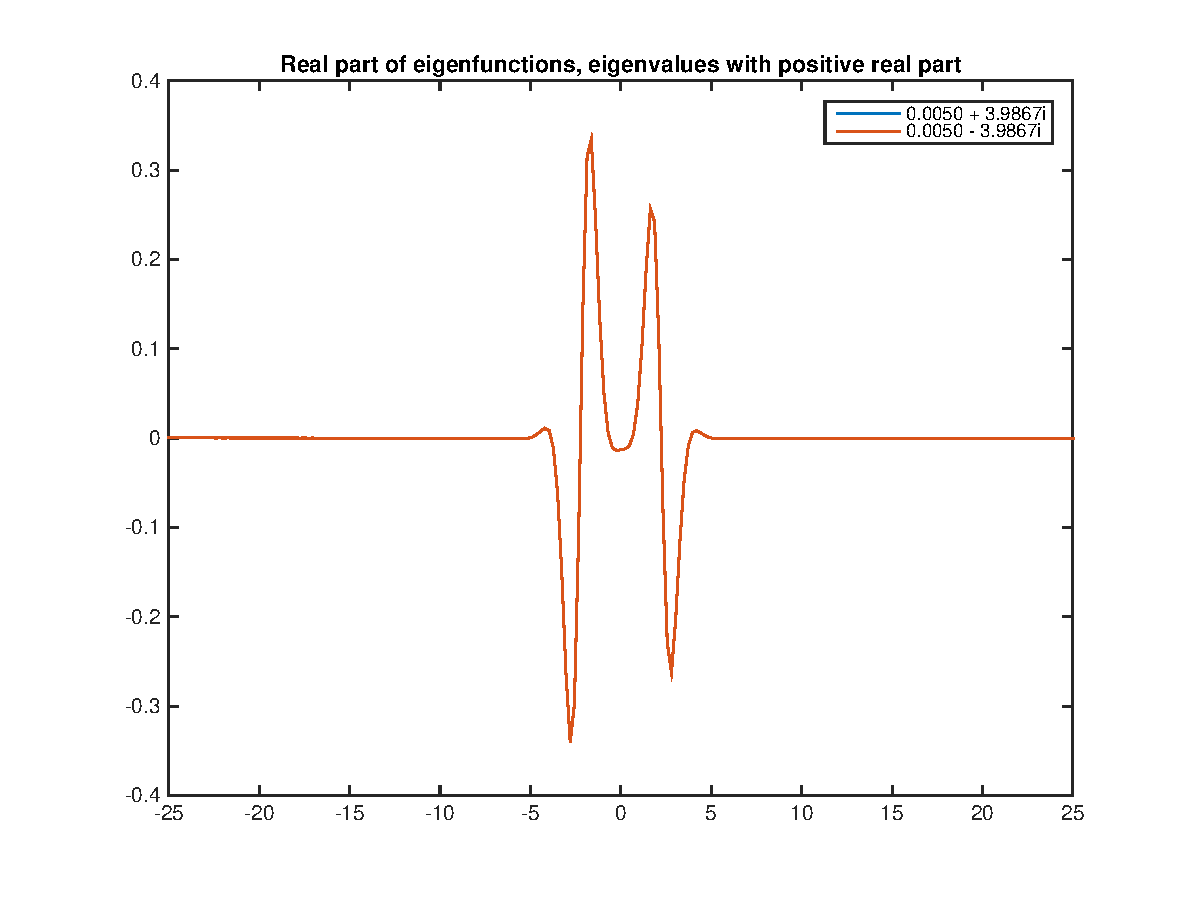
\includegraphics[width=8.5cm]{1500F_dp2_1195_eigposreal}
	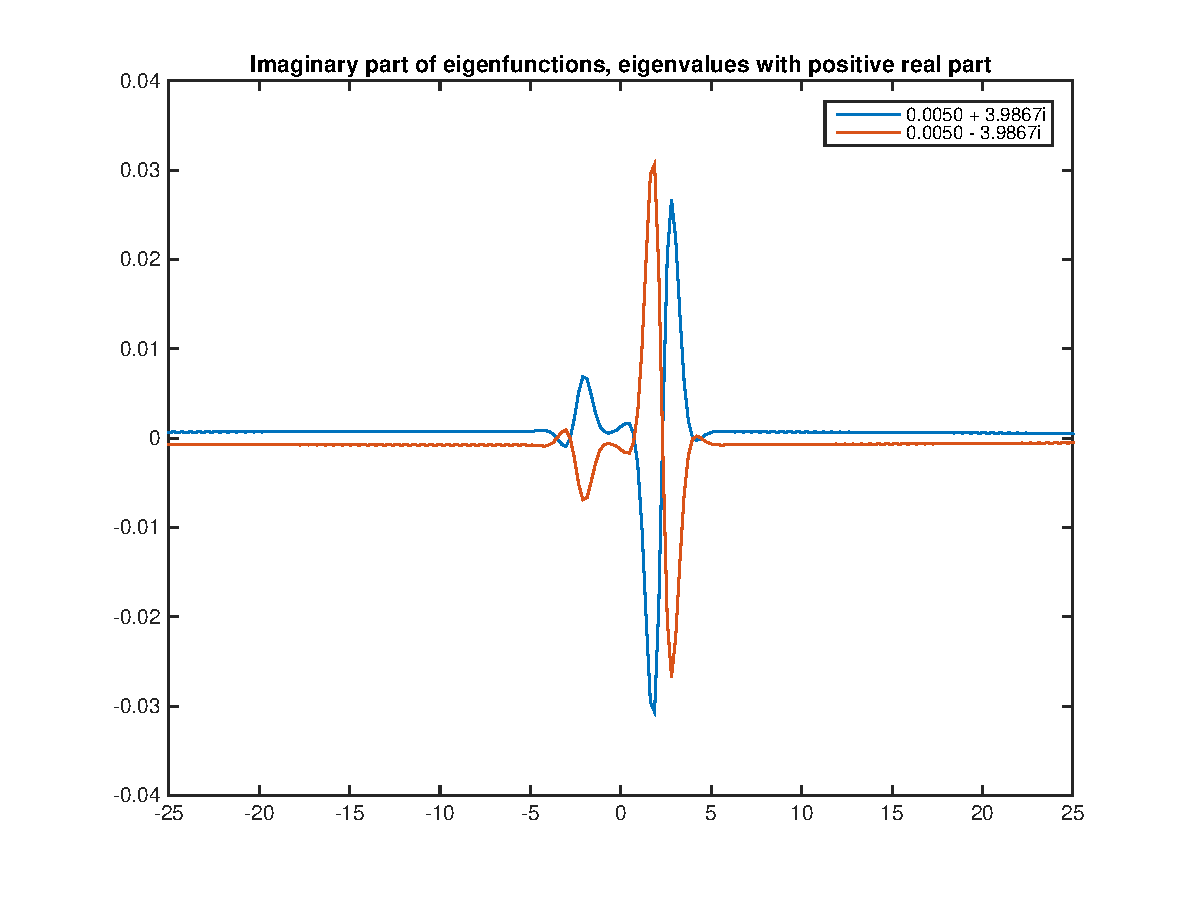
\includegraphics[width=8.5cm]{1500F_dp2_1195_eigposimag}
	\caption{Real and imaginary parts of eigenfunctions of Krein quartet eigenvalues with positive real part, double pulse 2(3), $c = 150$, Fourier spectral methods, $N = 1024$, $L = 119.5$. }
\end{figure}

\begin{figure}[H]
	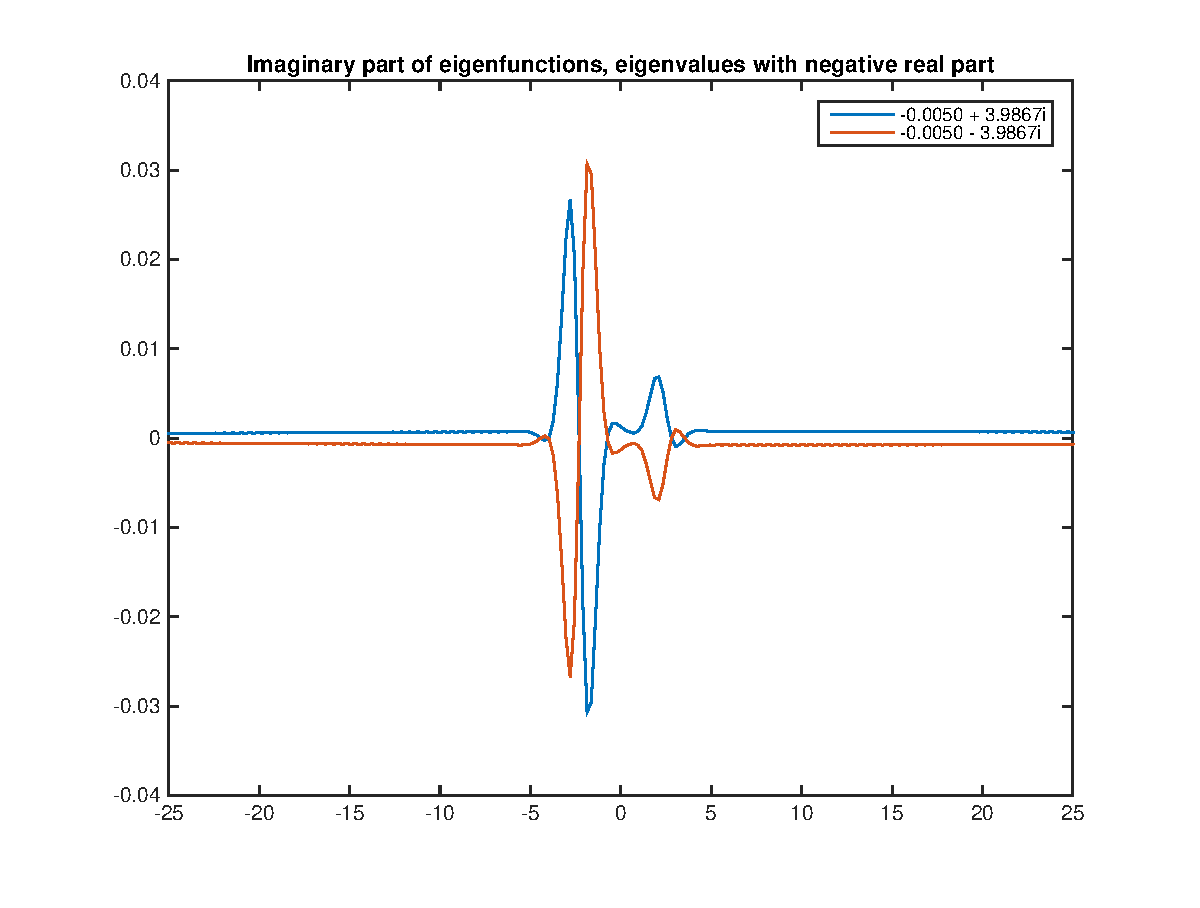
\includegraphics[width=8.5cm]{1500F_dp2_1195_eignegreal}
	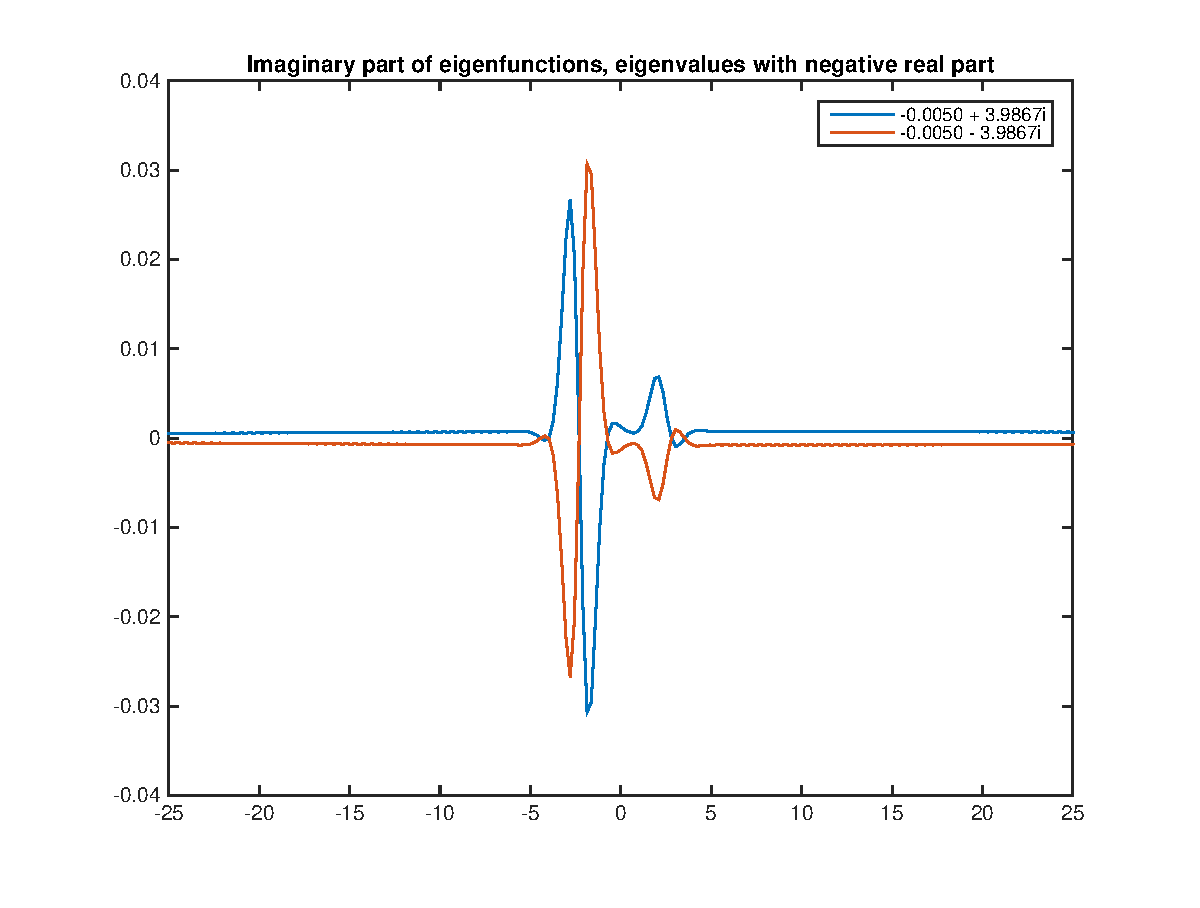
\includegraphics[width=8.5cm]{1500F_dp2_1195_eignegimag}
	\caption{Real and imaginary parts of eigenfunctions of Krein quartet eigenvalues with positive real part, double pulse 2(3), $c = 150$, Fourier spectral methods, $N = 1024$, $L = 119.5$. }
\end{figure}

These look about how we would expect (i.e. have the correct symmetries). For some reason the real parts decay to 0 at the ends (as we expect) but the imaginary parts do not (even if we look at the entire domain), so this is a little fishy.\\

Let's look at the Krein eigenvalues. Since the imaginary part of the quartet is $3.9867i$, we will look at the interval $z \in [15.8, 16.0]$. Note that we have two singularities (Krein eigenvalue 1 has one first, as before), but neither curve crosses 0, suggesting that there are no eigenvalues on the imaginary axis near there.

\begin{figure}[H]
	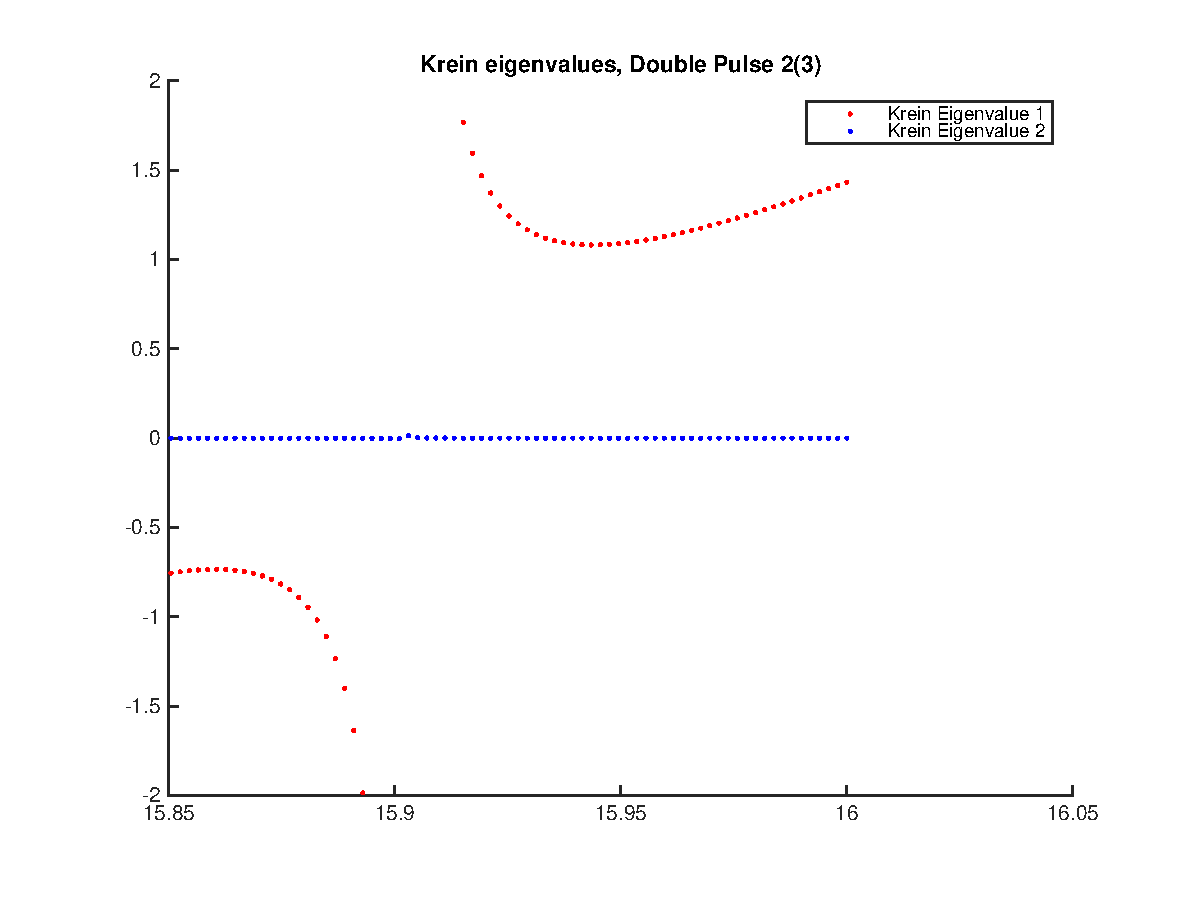
\includegraphics[width=8.5cm]{1500F_dp2_1195_krein1.eps}
	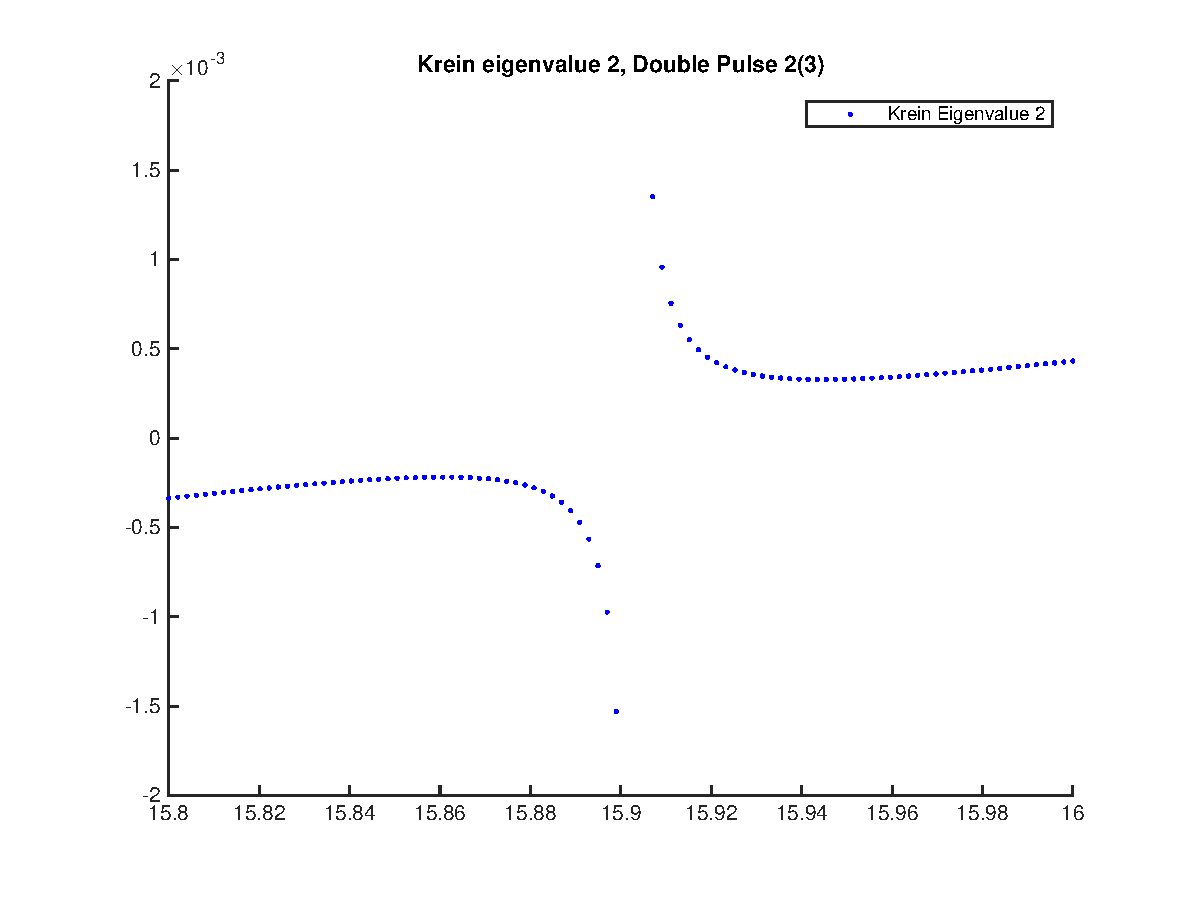
\includegraphics[width=8.5cm]{1500F_dp2_1195_krein2.eps}
	\caption{Krein eigenvalues 1 and 2 (left) and Krein eigenvalue 2 (right), double pulse 2(3), $c = 150$, Fourier spectral methods, $N = 1024$, $L = 119.5$. }
\end{figure}

Since $\lambda = 0.0050 + 3.9867i$ is in the first quadrant, the Krein matrix should be singular at $z = -\lambda^2 = 15.8934 - 0.0397i$. If we take the determinant of the Krein matrix at this value of $z$, we get $\det K(z) = -3.0678e-04 + 1.2304e-05i$ which is small, zero. Again, this is a little fishy, and we will return to this point later.\\

Finally, we by looking different values of $L$, we can actually see the alleged Krein collision take place. The eigenvalues collide and form a Krein quartet, which then collapses back to the imaginary axis. Here is a table showing this.

\begin{table}[H]
\begin{tabular}{l|l}
Domain length (L) & Eigenvalues \\ \hline
119.25 & $\pm 3.9924i, \pm 3.9894i$ \\
119.28 & $\pm 0.0017 \pm 3.9904i$\\ 
119.30 & $\pm 0.0024 \pm 3.9900i$\\
119.35 & $\pm 0.0036 \pm 3.9892i$\\
119.40 & $\pm 0.0043 \pm 3.9884i$\\
119.45 & $\pm 0.0047 \pm 3.9875i$\\
119.50 & $\pm 0.0050 \pm 3.9867i$\\
119.55 & $\pm 0.0051 \pm 3.9858i$\\
119.60 & $\pm 0.0051 \pm 3.9850i$\\
119.65 & $\pm 0.0049 \pm 3.9841i$\\
119.70 & $\pm 0.0046 \pm 3.9833i$\\
119.75 & $\pm 0.0041 \pm 3.9825i$\\
119.80 & $\pm 0.0033 \pm 3.9816i$\\
119.85 & $\pm 0.0018 \pm 3.9808i$\\
119.90 & $\pm 3.9776i, \pm 3.9823i$\\
\end{tabular}
\end{table}

We would like to know if this Krein collision is actually taking place, or whether this is just numerical error. It seems weird that the we would have a Krein collision producing a quartet which then collapses back to the imaginary axis. We would expect that once the quartet formed, it would persist for all higher values of $L$. As a verification, assume that we have an eigenvalue in the first quadrant of the complex plane, i.e. $\lambda = \alpha + \beta i$, with $\alpha, \beta > 0.$ Then the Krein matrix $K(z)$ should be singular at $z = -\lambda^2$. The value of $z$ we used above gave us a determinant which was small but not zero. Perhaps we could use \texttt{fsolve} to find this zero.\\

To to this, we first adapt the Krein matrix generation as follows. Since inverting large matrices is slow, we do not want to calculate $(R_2 - zS_2)^{-1}$ every time we take another step. We can speed things up by (approximately) a factor of 3 by doing the following two things:
\begin{enumerate}
	\item Since we know the Krein matrix is diagonal, only compute the diagonal entries.
	\item Instead of inverting $(R_2 - zS_2)^{-1}$ to compute $y = (R_2 - zS_2)^{-1} x$, use Matlab's linear solver to solve $x = (R_2 - zS_2) y$, where here $x = P R \phi_j$ 
\end{enumerate}

Before we do this, we would like to note that using \texttt{fsolve} for finding eigenvalues works really well. We can confirm our results above by doing this (not shown). Interesting things to note (for our initial case of double pulse 2(3), $c = 10$, $L = 25$, Fourier spectral methods, $N = 256$:
\begin{enumerate}
	\item Unless we start really near one of the essential spectrum eigenvalues, \texttt{fsolve} will give us the interaction eigenvalue. We can start just about anywhere (zero, large positive and negative numbers), and \texttt{fsolve} will give us the interaction eigenvalue. In this case, both Krein eigenvalues are tiny (order 1e-10 or smaller).
	\item If we want to get the essential spectrum eigenvalue, we have to start quite near it. Note from the cartoon and plots above, Krein eigenvalue 1 crosses zero on the way down to a singularity, while Krein eigenvalue 2 crosses on a gentle downslope. Thus if we want to show that both Krein eigenvalues are zero (to reasonable accuracy), we need to start the solver on the left side since the solver does not cross the singularity. The best way to do this is to use the solver on Krein eigenvalue 1, rather than the determinant. If we do this, we get that Krein eigenvalue 1 is order 1e-6 and Krein eigenvalue 2 is order 1e-8, and the Krein matrix has determinant of order 1e-13.
\end{enumerate} 

So we have found that the Krein matrix (via its determinant) is highly effective for finding the interaction eigenvalues, and also is effective in finding the essential spectrum eigenvalues, as long as we know roughly where they are so we can start the solver at the right initial point.\\

Now we return to our alleged Krein quartet. Recall that for double pulse 2(3), $c = 150$, $L = 119.5$, Fourier spectral methods, $N = 1024$ Matlab's \texttt{eig} gives us a quartet of eigenvalues at $\pm 0.0050 \pm 3.9867i$. We want the eigenvalue in the first quadrant, which corresponds to $z = 15.8938 - 0.0399i$. Let's see how \texttt{fsolve} does with this. Recall that for the initial guess from \texttt{eig}, we have $|\det K(z) =  3.0811e-04$.

\begin{table}[H]
\begin{tabular}{l|lll}
Initial guess & Output & $|\det K(z)|$ & Krein eigenvalues \\ \hline
15.8938 - 0.0399i & 15.8663 - 0.0399i & 2.6442e-04 & -0.4523 - 0.6969i, -1.3452e-04 - 2.8846e-04i \\
15.8938 & 15.8606 & 1.5988e-04 & -0.7343, -2.1773e-04 \\
\end{tabular}
\end{table}

Even with \texttt{fsolve}, we can hardly improve $|\det K(z)|$ when starting at the value suggested by \texttt{eig}. In fact, we get a slightly better value for $|\det K(z)|$ if we start with the real part of $z$, i.e. $\lambda$ is pure imaginary. We still do not get better than order 1e-4. Since the Krein matrix usually does much better than this, we conclude that it is unlikely that this quartet actually occurs.\\

Let's look at the eigenfunctions corresponding to the essential spectrum eigenvalues and the interaction eigenvalues before and after the collision.\\

First, we look before the collision, i.e. double pulse 2(3), $c = 150$, Fourier spectral methods, $N = 1024$, $L = 119$. Here is a plot of the two eigenfunctions (for positive imaginary part only).

\begin{figure}[H]
	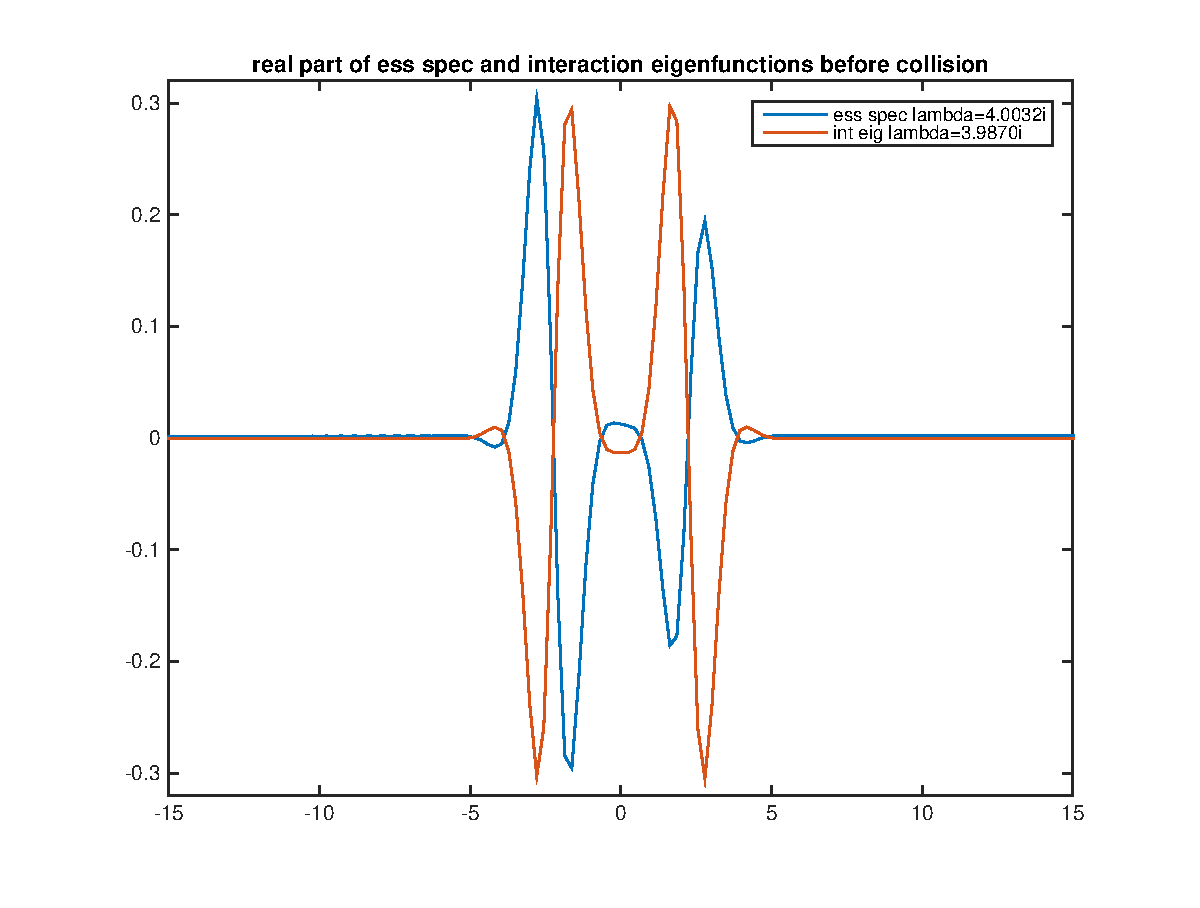
\includegraphics[width=8.5cm]{eigbeforecollision1.eps}
	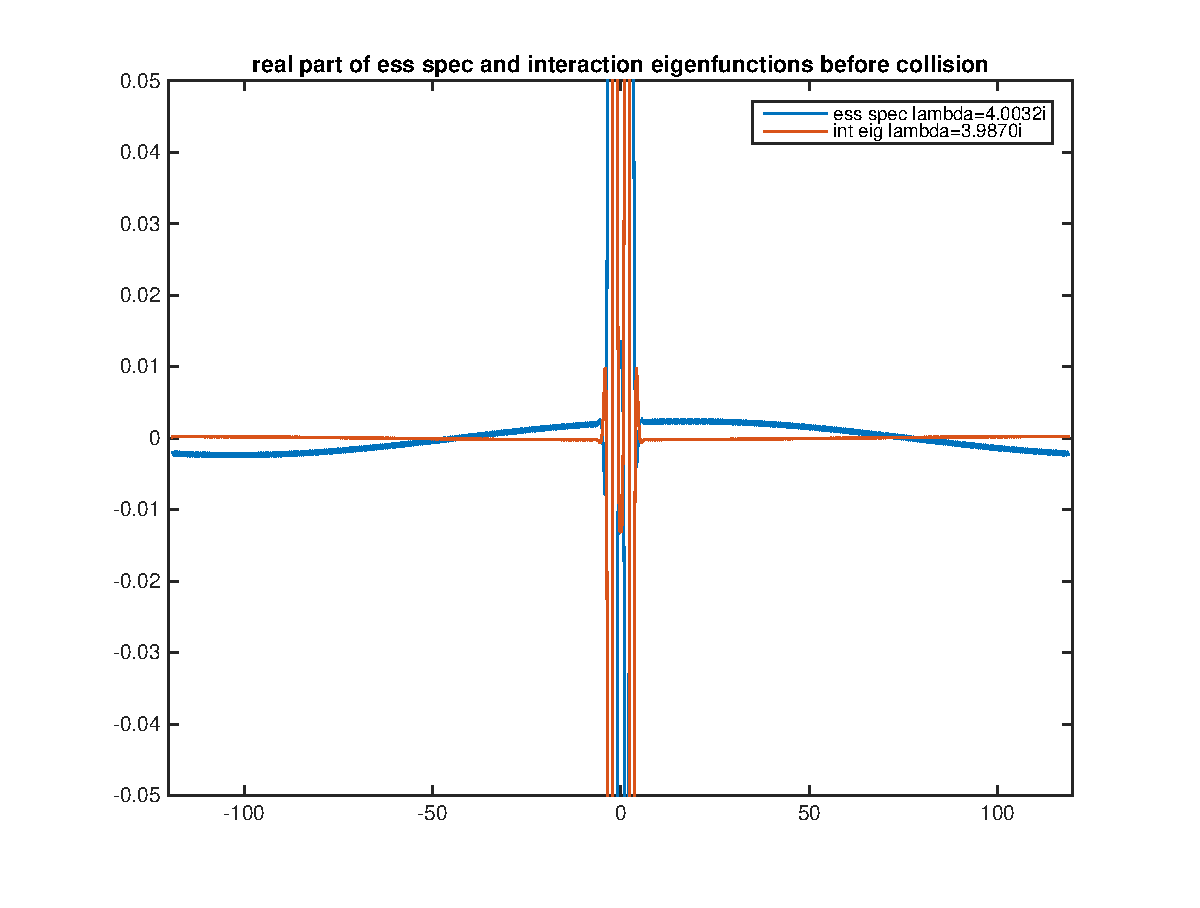
\includegraphics[width=8.5cm]{eigbeforecollision2.eps}
	\caption{Real part of eigenfunctions corresponding to the essential spectrum eigenvalues and the interaction eigenvalues before the collision. Left shows center, right shows tails. Double pulse 2(3), $c = 150$, Fourier spectral methods, $N = 1024$, $L = 119$. }
\end{figure}

\begin{figure}[H]
	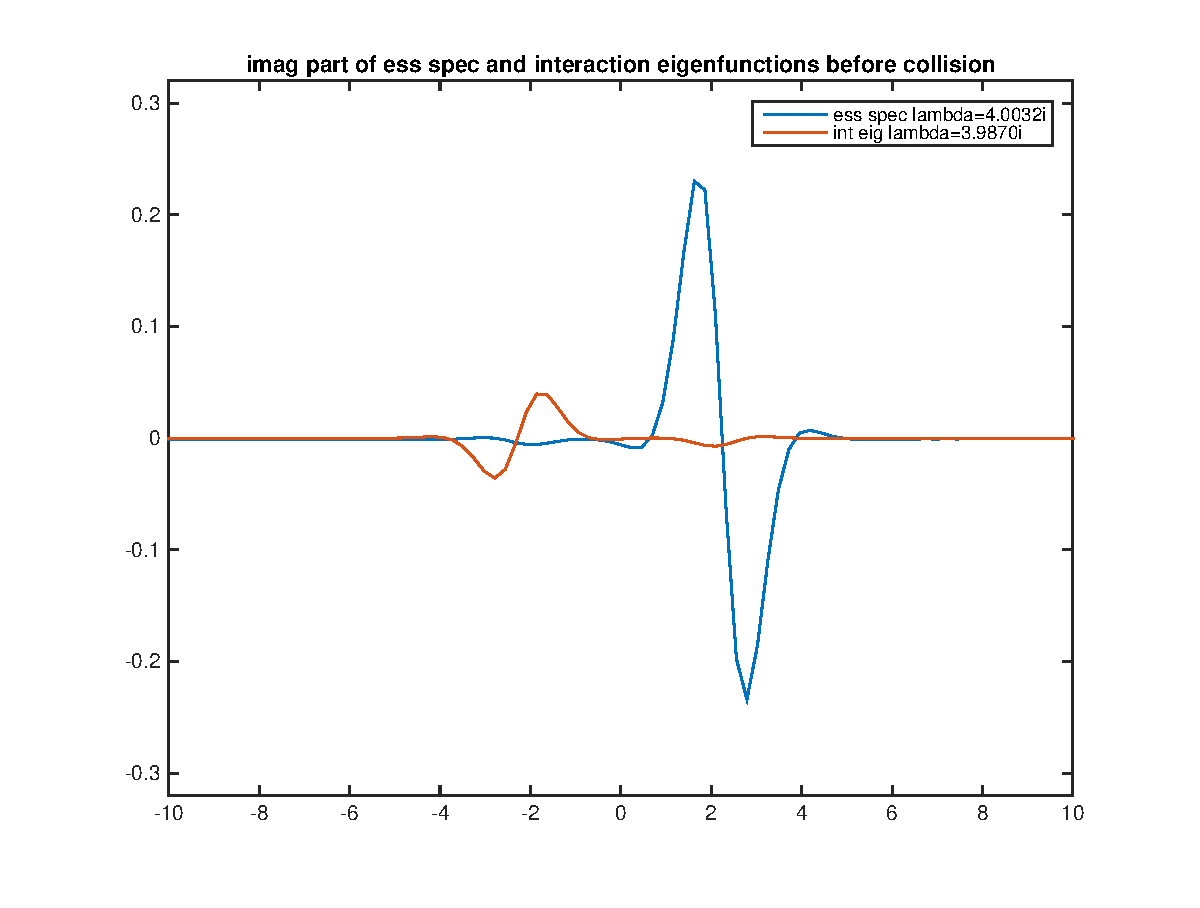
\includegraphics[width=8.5cm]{eigbeforecollisionimag1.eps}
	\caption{Imaginary part of eigenfunctions corresponding to the essential spectrum eigenvalues and the interaction eigenvalues before the collision. Double pulse 2(3), $c = 150$, Fourier spectral methods, $N = 1024$, $L = 119$. }
\end{figure}


Integrating numerically from $-L$ to $L$ (using the discrete norm or left Riemann sum, i.e. summing up the function values at the grid points and multiplying by the grid size) we have -3.2925e-13 + 7.4925e-13i (essential spectrum eigenfunction) and 1.0050e-13 - 3.2640e-13i (interaction eigenfunction).\\

Now we look after the collision, i.e. double pulse 2(3), $c = 150$, Fourier spectral methods, $N = 1024$, $L = 120$. Below is the plot of the two eigenfunctions.

\begin{figure}[H]
	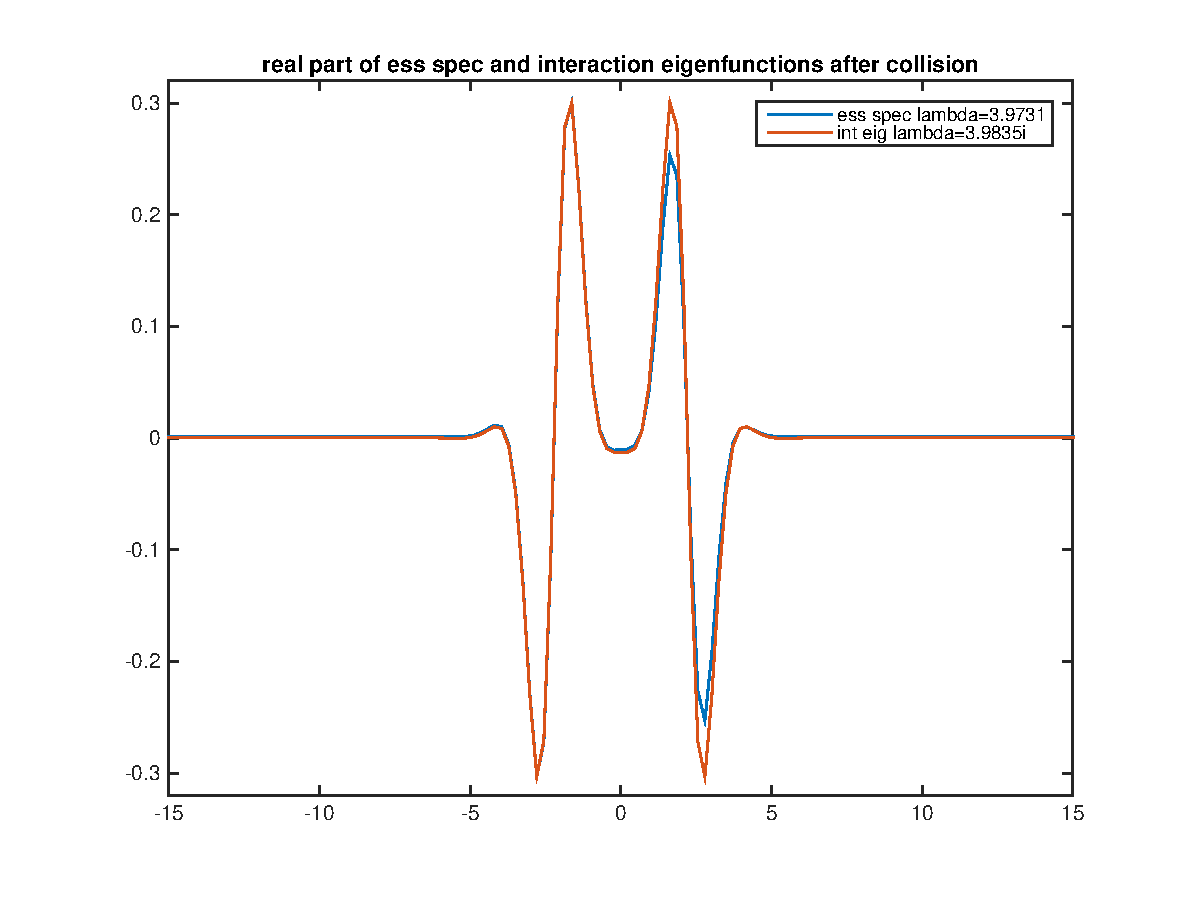
\includegraphics[width=8.5cm]{eigaftercollision1.eps}
	\includegraphics[width=8.5cm]{eigaftercollision2.eps}
	\caption{Real part of eigenfunctions corresponding to the essential spectrum eigenvalues and the interaction eigenvalues after the collision. Left shows center, right shows tails. Double pulse 2(3), $c = 150$, Fourier spectral methods, $N = 1024$, $L = 120$. }
\end{figure}

\begin{figure}[H]
	\includegraphics[width=8.5cm]{eigaftercollisionimag1.eps}
	\caption{Imaginary part of eigenfunctions corresponding to the essential spectrum eigenvalues and the interaction eigenvalues after the collision. Double pulse 2(3), $c = 150$, Fourier spectral methods, $N = 1024$, $L = 120$. }
\end{figure}

Integrating numerically from $-L$ to $L$ we have 7.4441e-13 - 3.1641e-12i (essential spectrum eigenfunction) and f-1.0170e-13 - 3.0413e-12i (interaction eigenfunction).\\

The interaction eigenfunction looks unchanged, whereas the gap between the two (asymmetric) peaks in the essential spectrum eigenfunction has narrowed significantly. For the imaginary part of the interaction eigenfunction, we should be able to multiply it by a unit complex number to ``rotate'' it so that the imaginary part is odd and the real part is even. We should be able to do that for the essential eigenfunction as well. So let's do it. Here are the eigenfunctions before the collision after ``rotation''.

\begin{figure}[H]
	\includegraphics[width=8.5cm]{eigbeforecollisionrealrotate1.eps}
	\includegraphics[width=8.5cm]{eigbeforecollisionimagrotate1.eps}
	\caption{Real and imaginary parts of eigenfunctions corresponding to the essential spectrum eigenvalues and the interaction eigenvalues before the collision. Plots are after ``rotation'' by unit complex number so that real part is even and imaginary part is odd. Norm of both eigenfunctions is 1. Double pulse 2(3), $c = 150$, Fourier spectral methods, $N = 1024$, $L = 119$. }
\end{figure}

Here are the eigenfunctions after the collision after ``rotation''.

\begin{figure}[H]
	\includegraphics[width=8.5cm]{eigaftercollisionrealrotate1.eps}
	\includegraphics[width=8.5cm]{eigaftercollisionimagrotate1.eps}
	\caption{Real and imaginary parts of eigenfunctions corresponding to the essential spectrum eigenvalues and the interaction eigenvalues after the collision. Plots are after ``rotation'' by unit complex number so that real part is even and imaginary part is odd. Norm of both eigenfunctions is 1. Double pulse 2(3), $c = 150$, Fourier spectral methods, $N = 1024$, $L = 120$. }
\end{figure}

These look very similar (in the center of the plot range; the tails still look different as we see in the tail plot above). The real parts especially look similar. The two eigenfunctions can be distinguished if you look at the contours of the imaginary parts around 0. All the eigenfunctions plotted above have norm of 1.



\end{document}